\documentclass[UTF8]{ctexart}

\usepackage{subfiles}  

%下面的语句, 引入你的头部设置文件
\usepackage{C:/phpStorm_proj/02_myself_ID_EGO/+100_latex_all_math_sel/myPreamble} 
%必须是绝对路径,才能让各个tex在单独编译时使用到

\title{矩阵及其运算}


%---------------------------------


\begin{document}
	\tableofcontents % 生成目录
	\date{} % 若不写这句, 则默认也会渲染出日期, 所以我们要手动赋空值
	\maketitle  %这行代码, 让你前面的 title, author, date生效
	
	\section{矩阵}
	
	矩阵一般用大写字母来表示. 比如 A, B, C, E. (D留给了行列式.) \\
	
	【矩阵和行列式的区别】:\\
	\begin{tabular}{|p{0.5\textwidth}|p{0.5\textwidth}|}
		\hline
		行列式 D & 矩阵 Matrix  \\
		\hline
		本质是个``数" & 是张``数表"  \\
		\hline
		符号, 用竖线包围表示, 即 |...| &   用 [] 或 () 包围. 几乎不用大括号.\\
		\hline
		必定是方形的, 即 行数=列数 &  行列数无要求. \\
		\hline
	\end{tabular} \\

	【元素都是0的矩阵, 叫零矩阵, 记作0】: \\
	
	【负矩阵】: 所有元素, 都取其负数的矩阵, 叫负矩阵. 记为 -A. \\
	
	【单位阵】: 即``主对角线"上元素都是1, 其他都是0的矩阵.  记作 E 或 I.\\
	记忆方法:  \\
	- 主对角线, 是下坡 $\backslash$ \\
	- 次对角线, 是上坡 / \\
	
	注意: \textbf{只有``方阵", 才有``主对角线"的概念.} 不是方阵, 就没有主对角线.\\
	
	$
	E\text{或}I=\underset{\text{单位阵}}{\underbrace{\left[ \begin{matrix}
				1&		&		\\
				&		\ddots&		\\
				&		&		1_{}\\
			\end{matrix} \right] }}
	$ \\
	
	【只有一个元素的矩阵, 书写它时可以不带矩阵括号】:\\
	如: [5]=5 \\
	
	【同型矩阵】: \\
	即两个矩阵A,B, 若A的行数=B的行数,  A的列数也=B的列数, 则它们就叫``同型矩阵". \\
	如: $A_{3×5}$ 和  $B_{3×5}$, 就是同型矩阵. 它们的形状是一样的. \\
	
	若同型矩阵中, 对应元素都相等, 则这两个矩阵相等. 换言之, \textbf{两个矩阵相等的前提, 是它们必须是``同型矩阵".} \\
	
	所以, 两个零矩阵, 不一定相等. 因为它们不一定是同型的. 如:\\
	$	0_{2×2}\ne 0_{2×3}	$\\
	

	\hrule


\section{矩阵的运算}
	
	\subsection{矩阵的加法, 减法}
	
	矩阵的加法, 只要把两个矩阵, 对应位置的元素直接相加就行了. 即: 	
	\begin{align*}
		\left[ \begin{matrix}
			a&		b&		c\\
			d&		e&		f\\
		\end{matrix} \right] +\left[ \begin{matrix}
			g&		h&		i\\
			j&		k&		l\\
		\end{matrix} \right] =\left[ \begin{matrix}
			a+g&		b+h&		c+i\\
			d+j&		e+k&		f+l\\
		\end{matrix} \right]
	\end{align*}
	
	\textbf{注意: 只有``同型矩阵"才能做相加减.} \\
	
	减法也是这个规律: 对应元素相减即可. 	
	\begin{align*}
	\left[ \begin{matrix}
		a&		b&		c\\
		d&		e&		f\\
	\end{matrix} \right] -\left[ \begin{matrix}
		g&		h&		i\\
		j&		k&		l\\
	\end{matrix} \right] =\left[ \begin{matrix}
		a-g&		b-h&		c-i\\
		d-j&		e-k&		f-l\\
	\end{matrix} \right]
\end{align*}	
	

	\hrule


\subsection{加法的性质}

- A+B = B+A \\
- (A+B) + C = A + (B+C) \\
- A + 0 = A  ← 注意, 零矩阵与A, 应该是``同型"的才能相加. (同时, 两个零矩阵, 也未必是同型的. 如 $0_{3 \times 5} \ne 0_{4 \times 7} $ \\
- A + (-A) = 0 \\
- $A + B = C \Longleftrightarrow  A = C - B$ \\
	
		\hrule
		
		
\subsection{矩阵的 数乘}	

	\begin{align*}
		k\left[ \begin{matrix}
			1&		2&		3\\
			4&		5&		6\\
			7&		8&		9\\
		\end{matrix} \right] =\left[ \begin{matrix}
			1k&		2k&		3k\\
			4k&		5k&		6k\\
			7k&		8k&		9k\\
		\end{matrix} \right]
	\end{align*}
		
		
就是把数字k, 乘给矩阵中每一个元素身上.\\

反过来说, 就是: \textbf{若矩阵中的所有元素, 都有同一个公因子, 则该公因子提到矩阵外, 只需提``一次".} \\
(\textbf{注意: 行列式中的公因子, 是``每行提一次"的.})\\


\hrule



\subsection{数乘的性质}	

- k(A+B) = kA + kB \\
- (k+l)A = kA + lA \\
- $k(lA) = (k \cdot l)A$  ← 两个数K和L, 可以先结合, 再去乘以矩阵A \\


\hrule


\subsection{矩阵的 乘法}	

\begin{align*}
	\left[ \begin{matrix}
		a&		b\\
		\hline
		c&		d\\
	\end{matrix} \right] 
\cdot 
\left[ \begin{array}{c|cc}
		e&		f\\
		g&		h\\
	\end{array} \right] =\left[ \begin{matrix}
		ae+bg&		A\text{行}1*B\text{列}2\\
		A\text{行}2*B\text{列}1&		A\text{行}2*B\text{列}2\\
	\end{matrix} \right]
\end{align*}


注意: \textbf{两个矩阵能相乘的前提是: 前面矩阵的列数 = 后面矩阵的行数.} \\
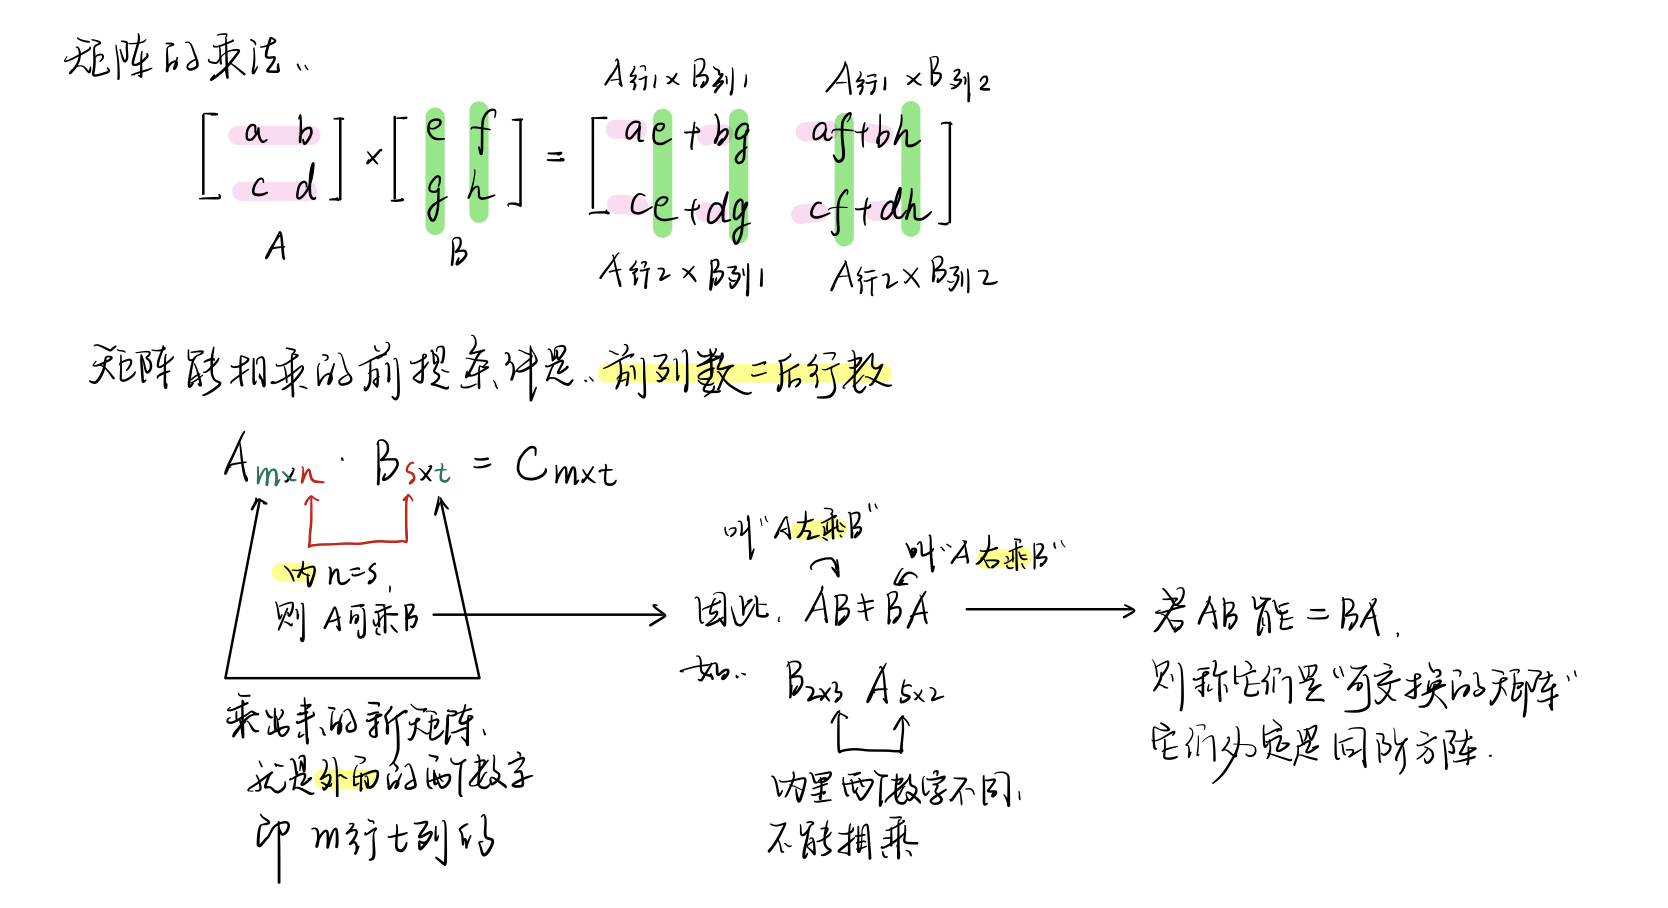
\includegraphics[width=1\textwidth]{img/0016.png} 

所以: \\
- 两个矩阵相乘的顺序不同的话, 结果就不同. 即: $AB \neq BA $ \\
- AB这个顺序能相乘, 不一定BA这个顺序也能相乘. 比如, $A_{5×2}B_{2×3}$ 是可以相乘的(它们内侧两个数字相同, 都是2), 能得到一个 5行3列的矩阵. 而顺序倒过来 $B_{2×3}A_{5×2}$就不能相乘了, 因为它们的内侧两个数字(前为3, 后为5)不相同. \\

所以, 我们要区分一下相乘的顺序: \\
- AB : 叫``A左乘B", 或``B右乘A" \\


单位阵E, 就相当于1的作用. 所以 AE = EA = A. 但是注意, 这里前后的两个单位阵E, 不是同一个E!  比如: \\
$A_{2×3}E_{3×3}=E_{2×2}A_{2×3}$\\
前面的E, 只能是3阶方阵. 后面的E, 只能是2阶方阵. 所以这两个E不是同一个单位阵. \\







\begin{myEnvSample}
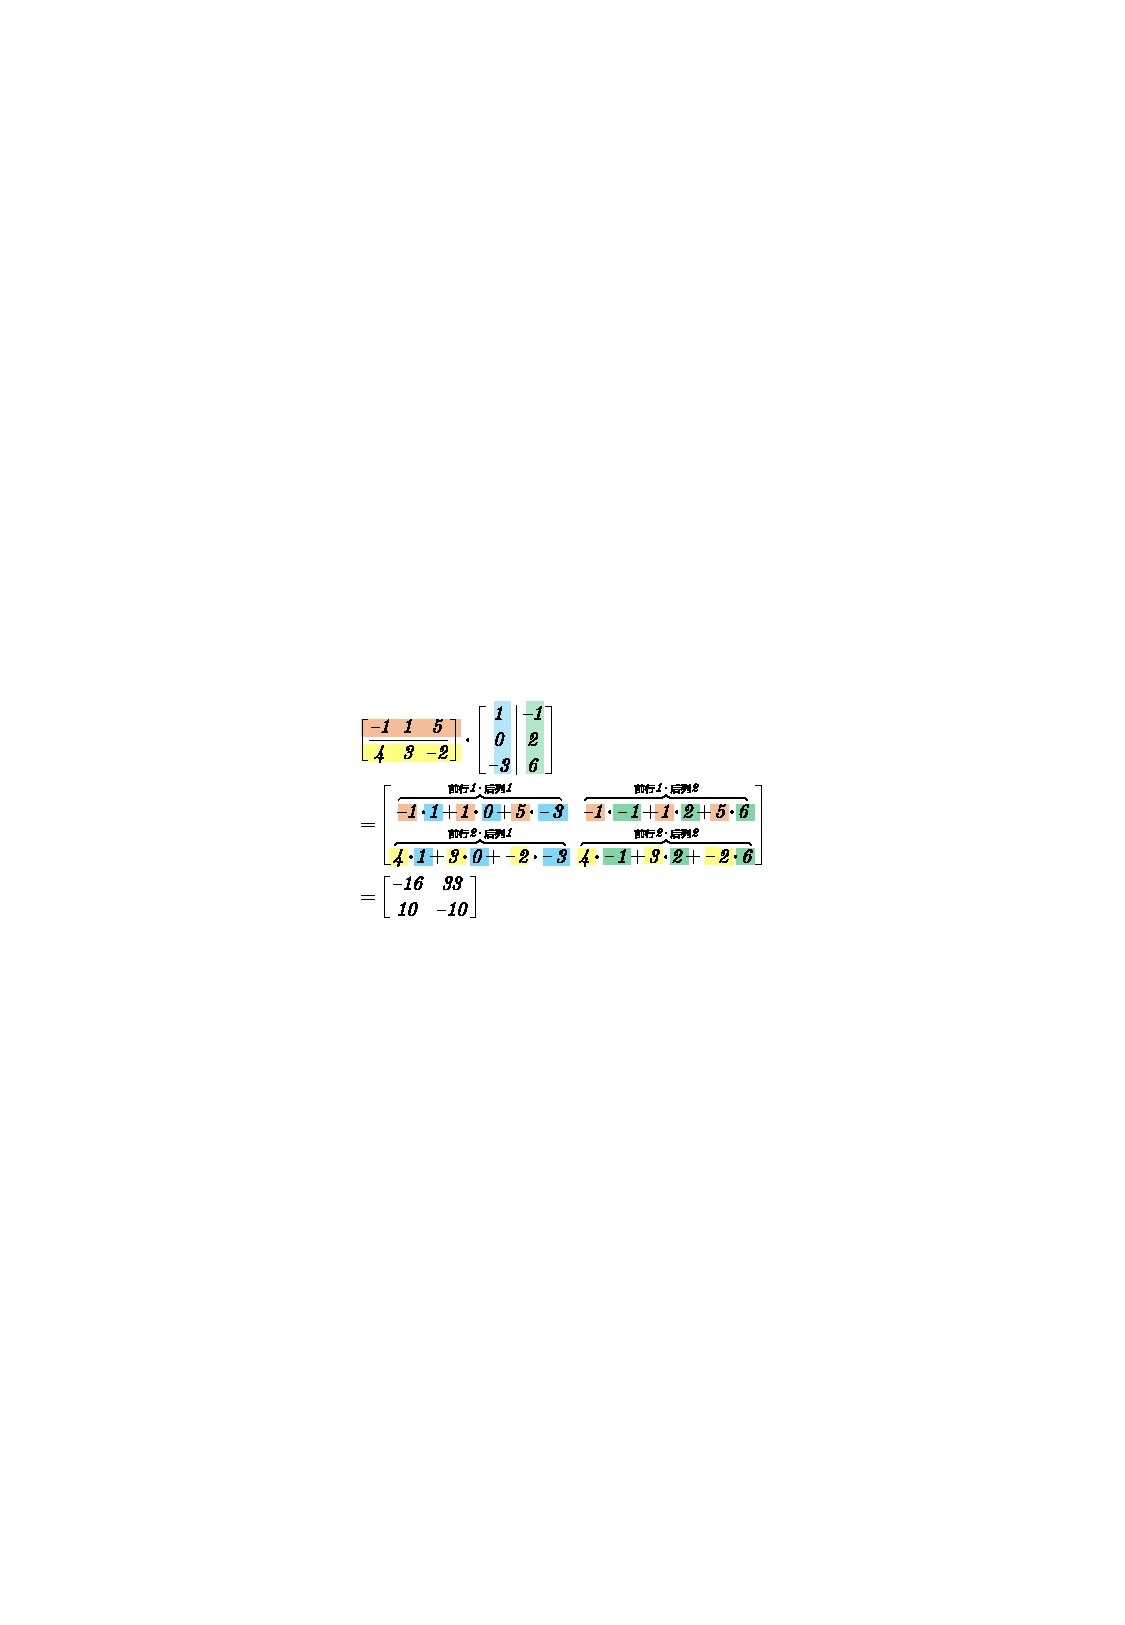
\includegraphics[width=0.6\textwidth]{img/0017.pdf}
\end{myEnvSample}

\hrule

\subsubsection{(1) AB=0 , 是推不出 A=0 或 B=0 的. (2) AB=AC, 且 $A =\neq 0 $, 是推不出 B=C 的.}

\begin{align*}
	& \text{有}	A=\left[ \begin{matrix}
		2&		0\\
		-1&		0\\
	\end{matrix} \right] ,\ B=\left[ \begin{matrix}
		0&		0\\
		1&		3\\
	\end{matrix} \right] ,\ C=\left[ \begin{matrix}
		0&		0\\
		2&		4\\
	\end{matrix} \right]\\
	&  \text{则:} AB=\left[ \begin{matrix}
		0&		0\\
		0&		0\\
	\end{matrix} \right] ,\ AC=\left[ \begin{matrix}
		0&		0\\
		0&		0\\
	\end{matrix} \right]\\
\end{align*}

从上面的结果, 我们可以得出这两个结论: \\
- \textbf{AB=0 , 是推不出 A=0 或 B=0 的.} \\
- \textbf{AB=AC, 且 $A \neq 0 $, 是推不出 B=C 的.} \\

\hrule

\subsubsection{一个矩阵, 与``零矩阵"相乘, 结果就是一个``新形状"的零矩阵}

如: $A_{4×3}O_{3×2}=O_{4×2}$ \\

\hrule

\subsubsection{一个矩阵X, 与``单位阵E"相乘(无论左乘还是右乘), 结果还是矩阵X本身. 即: AE=A, EB=B}

AE=A, EB=B \\

如: $
\underset{A}{\underbrace{\left[ \begin{matrix}
			3&		3&		3\\
			4&		1&		1\\
			5&		9&		9\\
		\end{matrix} \right] }}×\underset{E}{\underbrace{\left[ \begin{matrix}
			1&		&		\\
			&		1&		\\
			&		&		1\\
		\end{matrix} \right] }}=\underset{A}{\underbrace{\left[ \begin{matrix}
			3&		3&		3\\
			4&		1&		1\\
			5&		9&		9\\
		\end{matrix} \right] }}
$\\

\hrule

\subsection{矩阵乘法的运算规律}

\subsubsection{结合律: (AB)C = A(BC)} 

ABC的顺序, 在等号两边, 不变.\\


\subsubsection{分配律: (1) (A+B)C = AC+BC,  (2) C(A+B) = CA+CB} 

C在右边时, 分配进去, C还是在右边. \\
C在左边时, 分配进去, C还是在左边. \\


\subsubsection{ k(AB) = (kA)B = A(kB)} 

即 k乘以AB, 可以先和A结合来算, 也可以先和B结合来算. \\
并且无论k在哪, AB的左右顺序, 永远是AB. \\


\hrule

\subsubsection{矩阵乘法的例题}

\begin{myEnvSample}
求出 与$
A=\left[ \begin{matrix}
	1&		0\\
	1&		1\\
\end{matrix} \right] 
$ 可交换的所有矩阵.\\

设其可交换的矩阵 $
B=\left[ \begin{matrix}
	a&		b\\
	c&		d\\
\end{matrix} \right] \ 
$

B要能与A可交换, 它就必须满足: $A_n B_n = B_n A_n $, 即A和B是同阶的方阵.  \\

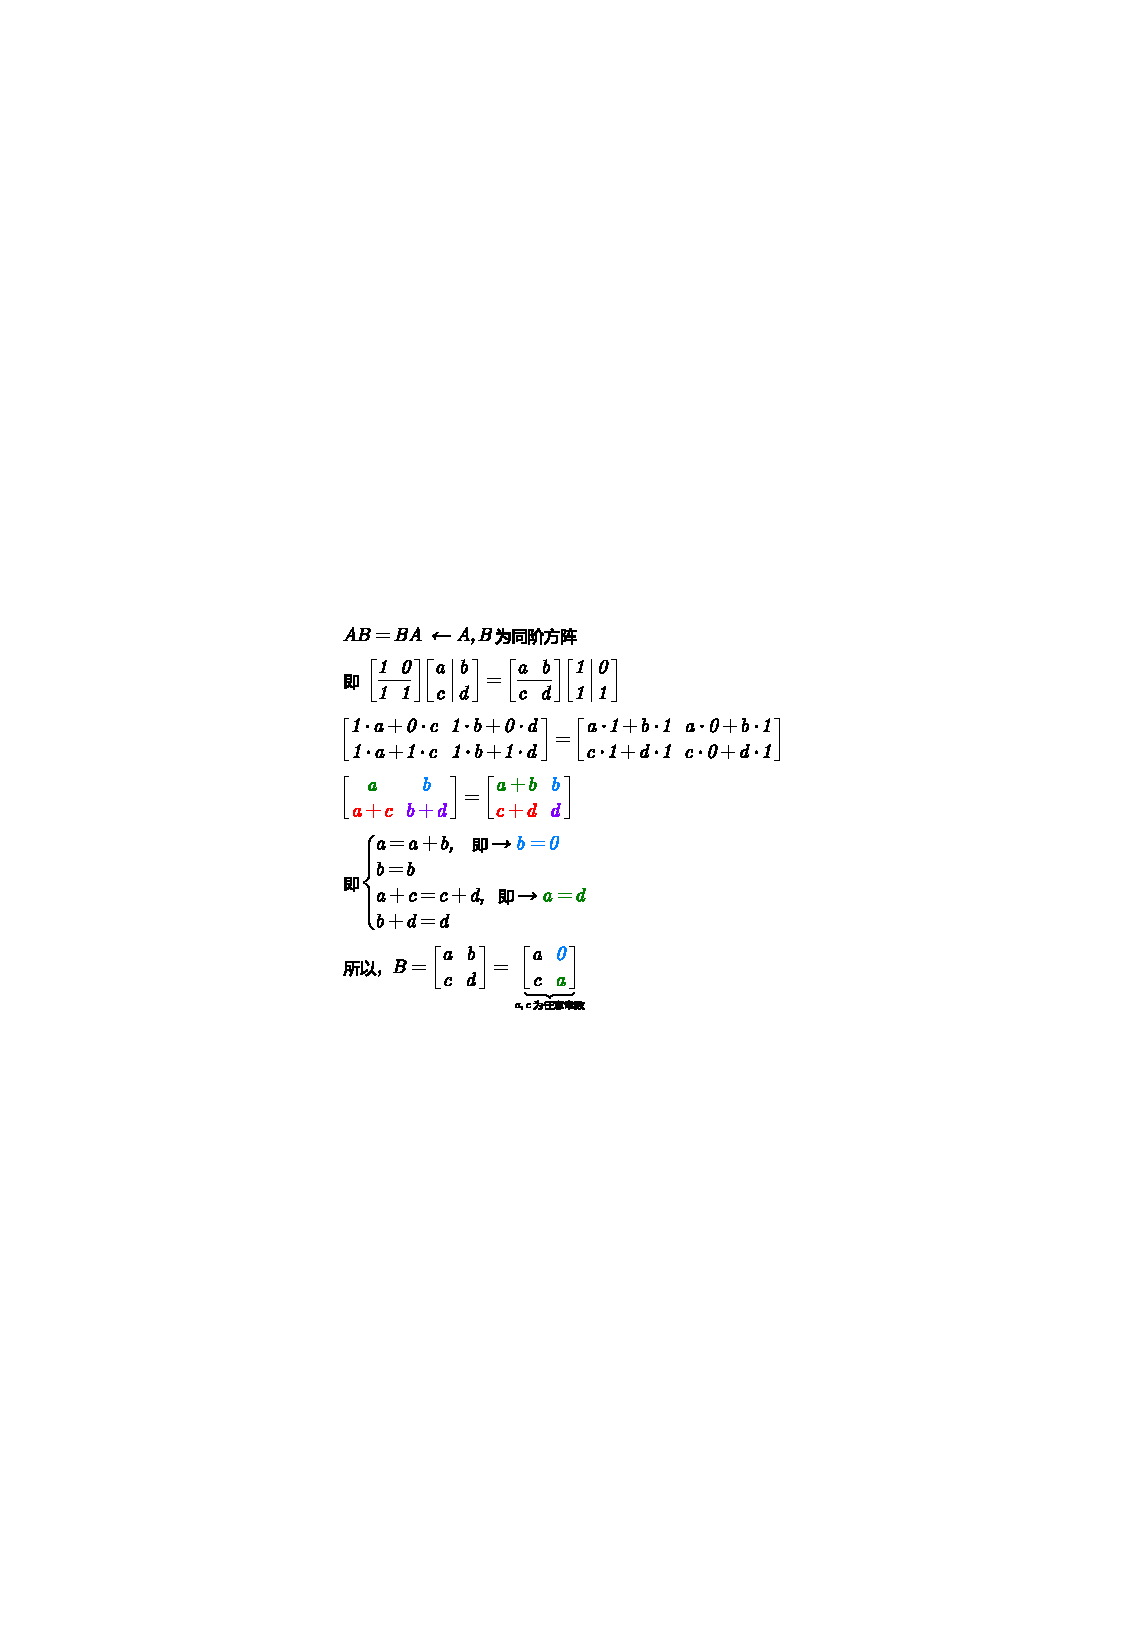
\includegraphics[width=0.7\textwidth]{img/0018.pdf}
\end{myEnvSample}




\begin{myEnvSample}
$
\left\{ \begin{array}{l}
	x_1=y_1-y_2\\
	x_2=y_1+y_2\\
\end{array} \right. \ \ \text{可以写成:\ }\left[ \begin{array}{c}
	x_1\\
	x_2\\
\end{array} \right] =\underset{\text{这两块,就是两个矩阵相乘}}{\underbrace{\left[ \begin{matrix}
			1&		-1\\
			\hline
			1&		1\\
		\end{matrix} \right] \left[ \begin{array}{c}
			y_1\\
			y_2\\
		\end{array} \right] }}
$
\end{myEnvSample}


\hrule

\subsection{矩阵, 幂的运算}
\subsubsection{$A^k=A\cdot A\cdot ...A\ ←\text{等号右边共}k\text{个}A$}

\begin{align*}
	A^k=\underset{k\text{个}A}{\underbrace{A\cdot A\cdot ...A}}
\end{align*}

\subsubsection{$A^0 = E$}

\subsubsection{$A^{k_1}A^{k_1}=A^{k_1+k_2}$}

\subsubsection{$\left( A^{k_1} \right) ^{k_2}=A^{k_1k_2}$}

\subsubsection{一般, $\left( AB \right) ^k\ne A^k B^k$ }

比如,  $\left( AB \right) ^2\ne A^2 B^2$ \\
因为: 等号左边 $\left( AB \right) ^2=\ ABAB$, 等号右边 $A^2B^2=\ AABB$, 而一般 $ABAB \ne AABB$. 因为虽然它们最左边都是A, 最右边都是B, 但是中间的两个矩阵相乘, BA一般就不等于AB了. 除非它们是可交换矩阵. \\

其他的: \\
$\left( A+B \right) ^2\ne A^2+2AB+B^2$  ← 这个, 一般也不相等 \\
$\left( A-B \right) ^2\ne A^2-2AB+B^2$  ← 这个, 一般也不相等 \\

\begin{myEnvSample}
问 $\left( A+E \right) ^2$ 是否等于 $A^2+2AE+E^2$ ?

\begin{align*}
		& \left( A+E \right) ^2=\left( A+E \right) \left( A+E \right)\\
	& =A\left( A+E \right) +E\left( A+E \right)\\
	& =A^2+\underset{=A}{\underbrace{AE}}+\underset{=A}{\underbrace{EA}}+\underset{=E}{\underbrace{E^2}}\\
	& =A^2+\underset{=2AE}{\underbrace{2A}}+E
\end{align*}

所以这个是对的. 相等. 
\end{myEnvSample}

同样, $\left( A-E \right) ^2 = A^2-2AE+E^2$ \\

\hrule

\subsubsection{矩阵的幂运算 例题}

\begin{myEnvSample}
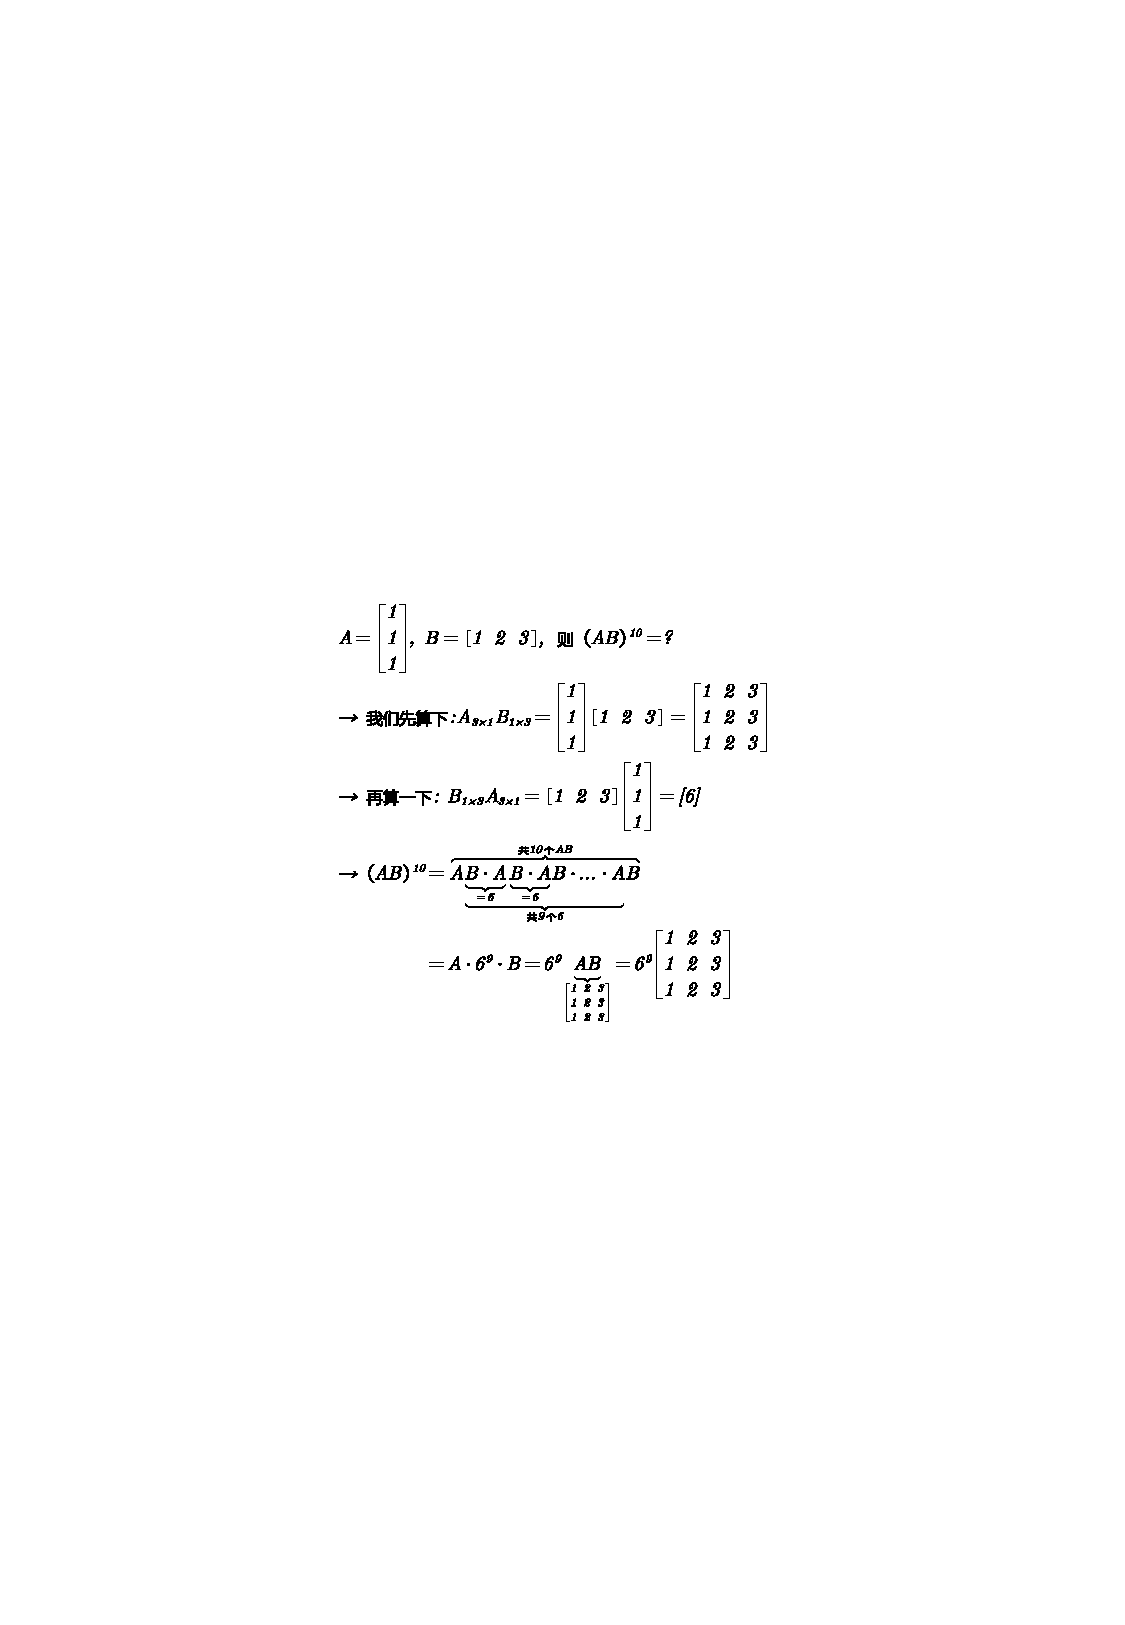
\includegraphics[width=0.6\textwidth]{img/0019.pdf}
\end{myEnvSample}


\hrule

\section{矩阵的转置}

$A_{m×n}$, 转置后, 就是$(A^T)_{n×m}$ \\

\subsection{性质: $(A^T) ^T = A$ }

\subsection{性质: $(A+B) ^T = A^T + B^T$ }

\subsection{性质: $(kA) ^T =  kA^T$ }

\subsection{\ding{72} 性质: $(AB) ^T = B^T A^T$  ← 注意AB顺序要颠倒 }

\subsection{性质: $(A_1 A_2 A_3 A_4)^T = A_4^T  A_3^T  A_2^T  A_1^T$ ← 顺序颠倒}

~\\
\hrule
~\\


\section{特殊矩阵 (都是方阵)}

\subsection{数量矩阵}

数量矩阵(或叫``纯量阵") scalar matrix : 就是``主对角线上"元素都是同一个数值,其余元素都是零. \\
即: \\
$
\left[ \begin{matrix}
	a&		&		&		\\
	&		a&		&		\\
	&		&		\ddots&		\\
	&		&		&		a\\
\end{matrix} \right]  
= aE
$\\

所以, 零矩阵, 和单位阵E, 都是特殊的``数量矩阵". \\

有性质: \\
(aE)B = B(aE) = aB \\


\hrule


\subsection{对角型矩阵}

对角矩阵 diagonal matrix : 主对角线元素无要求(可以不相等), 但之外的所有元素都为0.\\

即: 
\begin{align}
	A\ =\left[ \begin{matrix}
		\lambda _1&		&		&		\\
		&		\lambda _2&		&		\\
		&		&		\ddots&		\\
		&		&		&		\lambda _n\\
	\end{matrix} \right]
\end{align}

可记为: $A = diag(\lambda_1, \lambda2, ..., \lambda_n) $\\

所以, ``数量矩阵"(主对角线上的元素都相等), 只不过是一种特殊的``对角矩阵"罢了.\\




\subsubsection{diag × B : 对角阵元素在哪一行上, 就乘到B的相同行上去}

\begin{align}
	\left[ \begin{matrix}
		k_1&		&		\\
		\hline
		&		k_2&		\\
		\hline
		&		&		k_3\\
	\end{matrix} \right] \left[ \begin{matrix}
		1&		2&		3\\
		\hline
		2&		2&		2\\
		\hline
		8&		8&		8\\
	\end{matrix} \right] =\left[ \begin{matrix}
		1k_1&		2k_1&		3k_1\\
		\hline
		2k_2&		2k_2&		2k_2\\
		\hline
		8k_3&		8k_3&		8k_3\\
	\end{matrix} \right]
\end{align}

即: diag 在前, 就乘到后者的``行"上去. (前行,后列) \\
即: \textbf{左乘, 对应后面的行.}\\




\subsubsection{B × diag : 对角阵元素在哪一列上, 就乘到B的相同列上去}

\begin{align}
	\left[ \begin{array}{c|c|c}
		1&		2&		3\\
		2&		2&		2\\
		8&		8&		8\\
	\end{array} \right] \left[ \begin{array}{c|c|c}
		k_1&		&		\\
		&		k_2&		\\
		&		&		k_3\\
	\end{array} \right] =\left[ \begin{array}{c|c|c}
		1k_1&		2k_2&		3k_3\\
		2k_1&		2k_2&		2k_3\\
		8k_1&		8k_2&		8k_3\\
	\end{array} \right]
\end{align}

即: diag 在后, 就乘到前者的``列"上去. (前行,后列)\\
即: \textbf{右乘, 对应后面的列.} \\

\hrule


\subsection{上三角形矩阵}

upper triangular matrix \\

$
\left[ \begin{matrix}
	a_{11}&		a_{12}&		a_{13}&		a_{14}\\
	&		a_{22}&		a_{23}&		a_{24}\\
	&		&		\ddots&		a_{34}\\
	&		&		&		a_{44}\\
\end{matrix} \right] 
$ \\

性质: \\
- 上三角矩阵, 乘以系数后, 也是上三角矩阵 \\
- 上三角矩阵间的``加减法"和``乘法"运算的结果, 仍是上三角矩阵 \\
- 上三角矩阵的``逆矩阵", 也仍然是上三角矩阵 \\
- 上三角矩阵的行列式, 为``主对角线"元素相乘 


\subsection{下三角形矩阵}

$
\left[ \begin{matrix}
	a_{11}&		&		&		\\
	a_{21}&		a_{22}&		&		\\
	a_{31}&		a_{32}&		\ddots&		\\
	a_{41}&		a_{42}&		a_{43}&		a_{44}\\
\end{matrix} \right] 
$\\


\hrule


\subsection{对称矩阵: 有 $A^T = A$ ← 即对自己做转置, 依然等于自己.}

对称矩阵 Symmetric Matrices : 是以主对角线为对称轴, 上下元素对应相等. 即: $a_{ij}= a_{ji}$ \\

如:\\
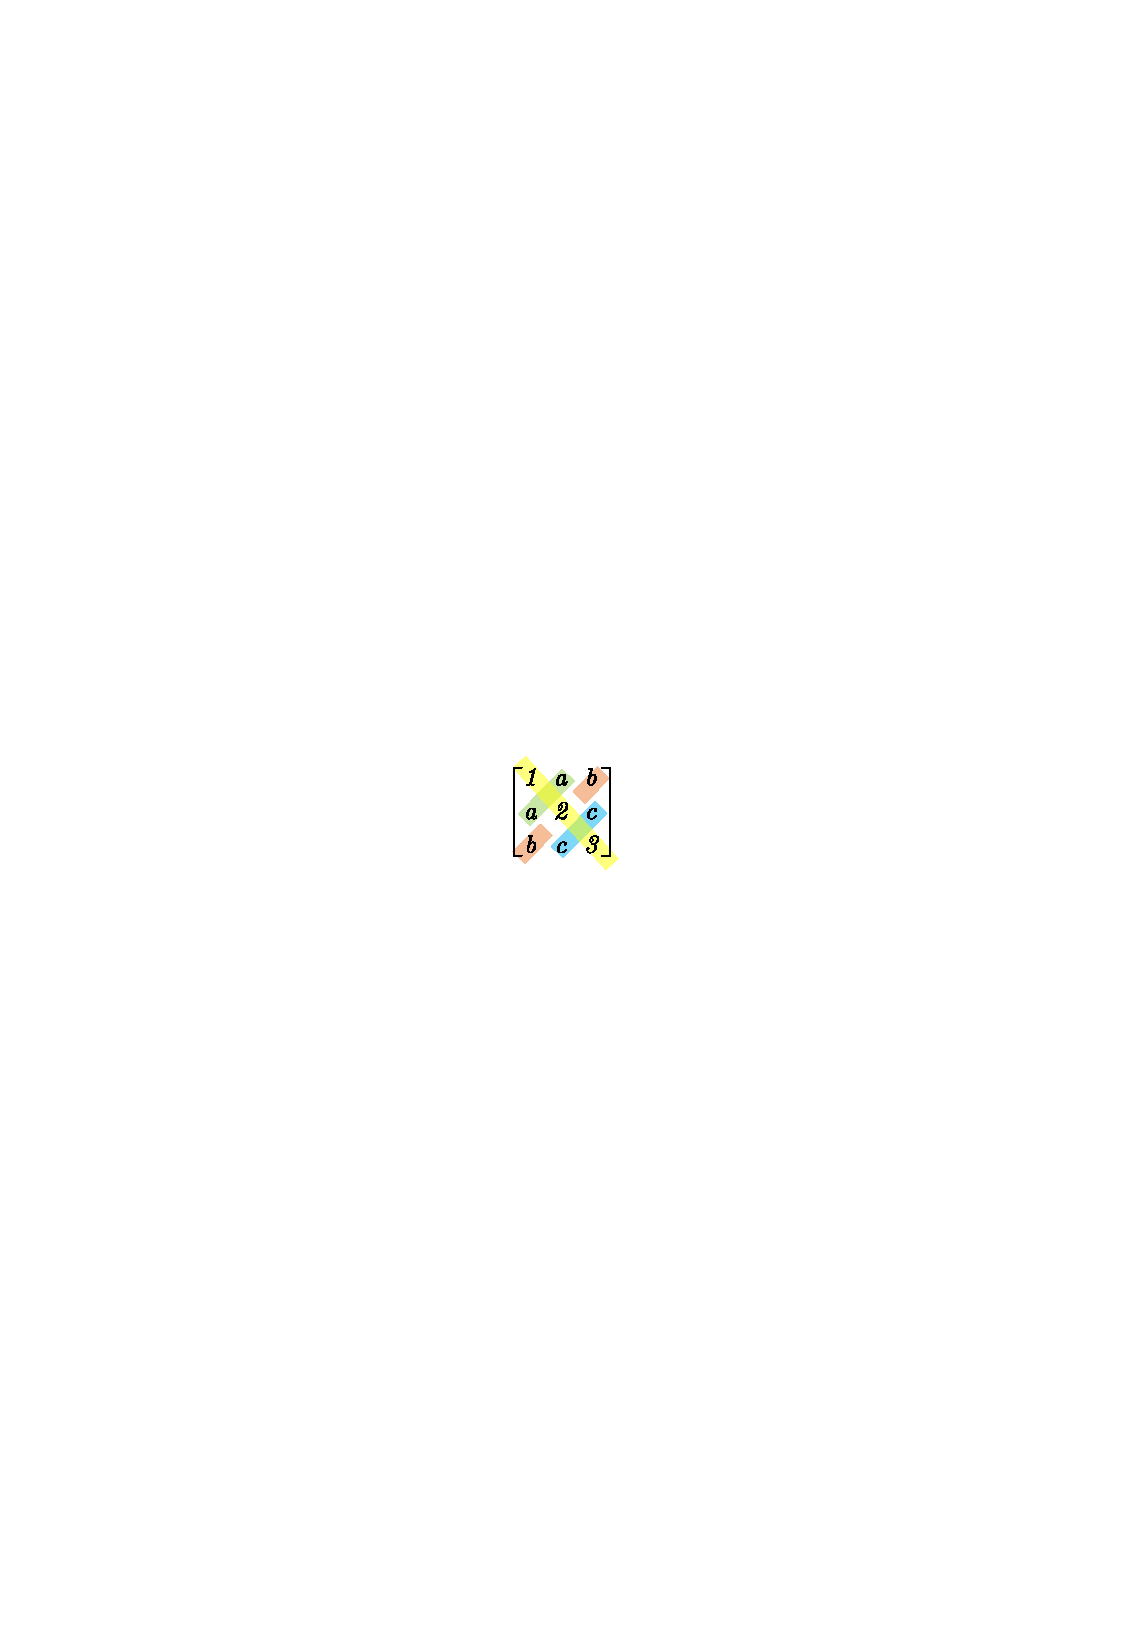
\includegraphics[width=0.15\textwidth]{img/0020.pdf}\\

对称矩阵, 有性质: $A^T = A$ \\



\begin{myEnvSample}
	注意: 下面例题中的字打错了, 不是``互为", 而是``都是". \\
	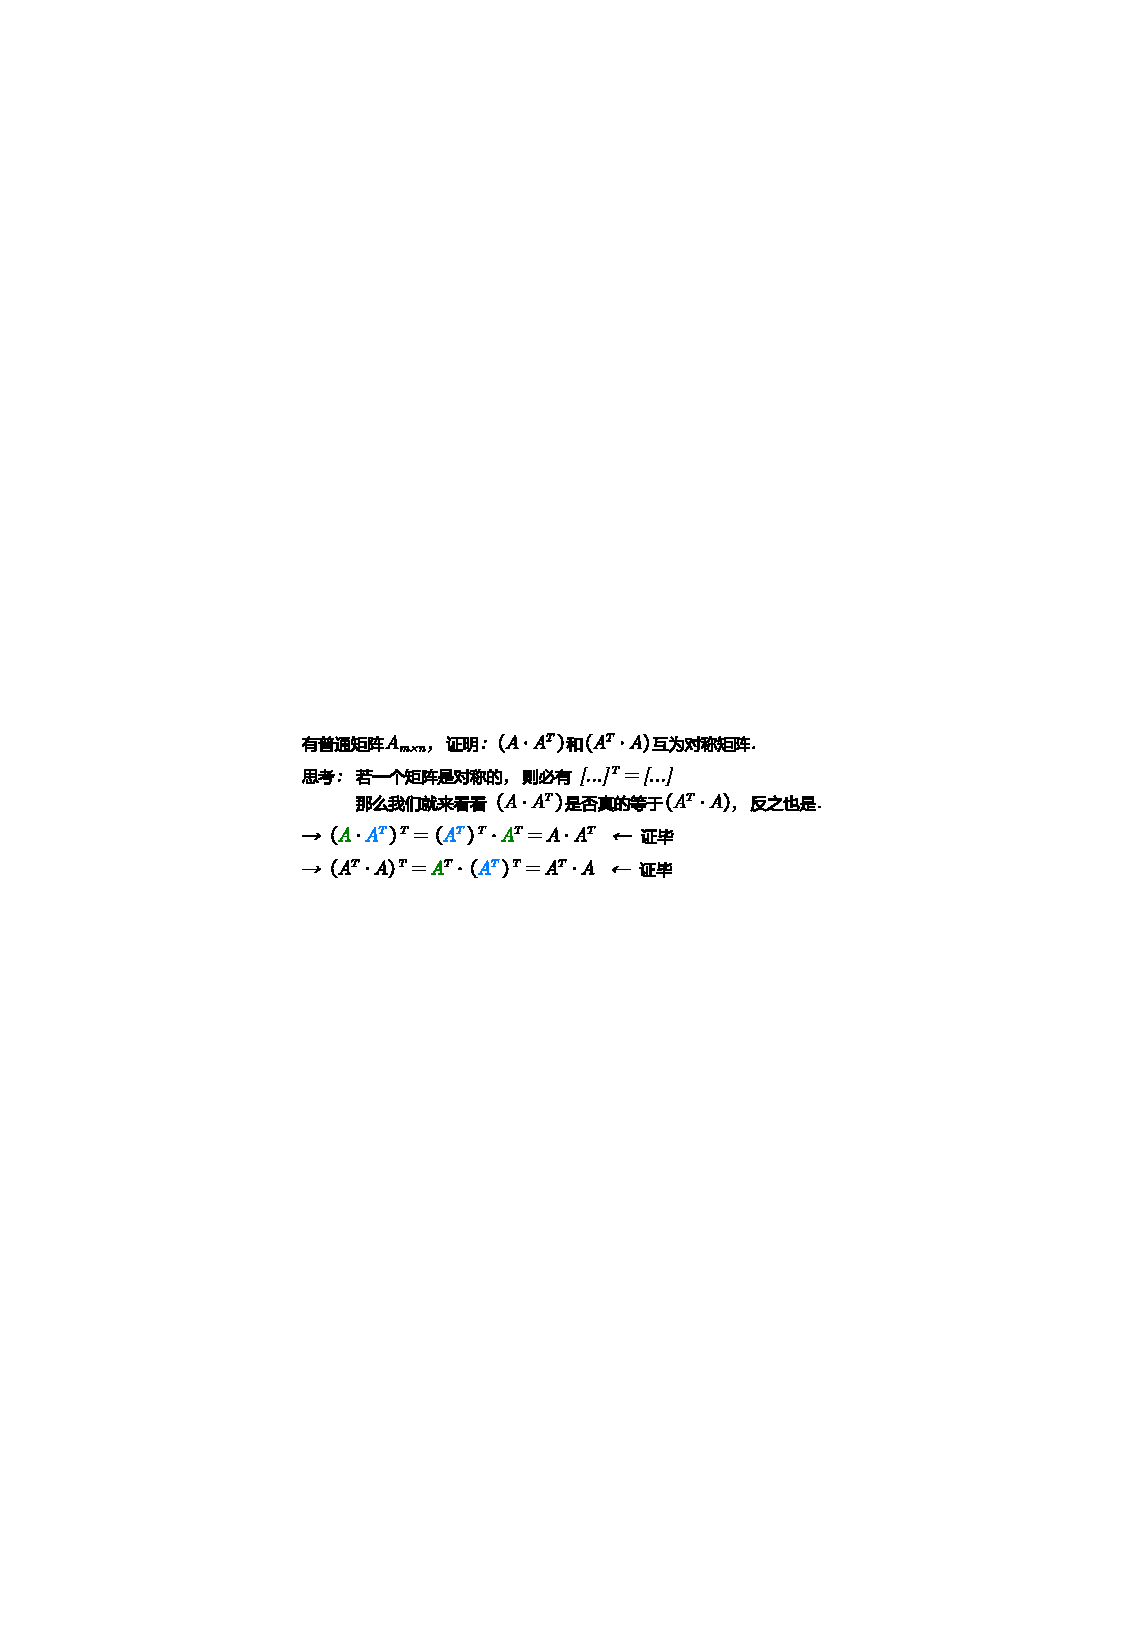
\includegraphics[width=0.75\textwidth]{img/0021.pdf}
\end{myEnvSample}



\begin{myEnvSample}
	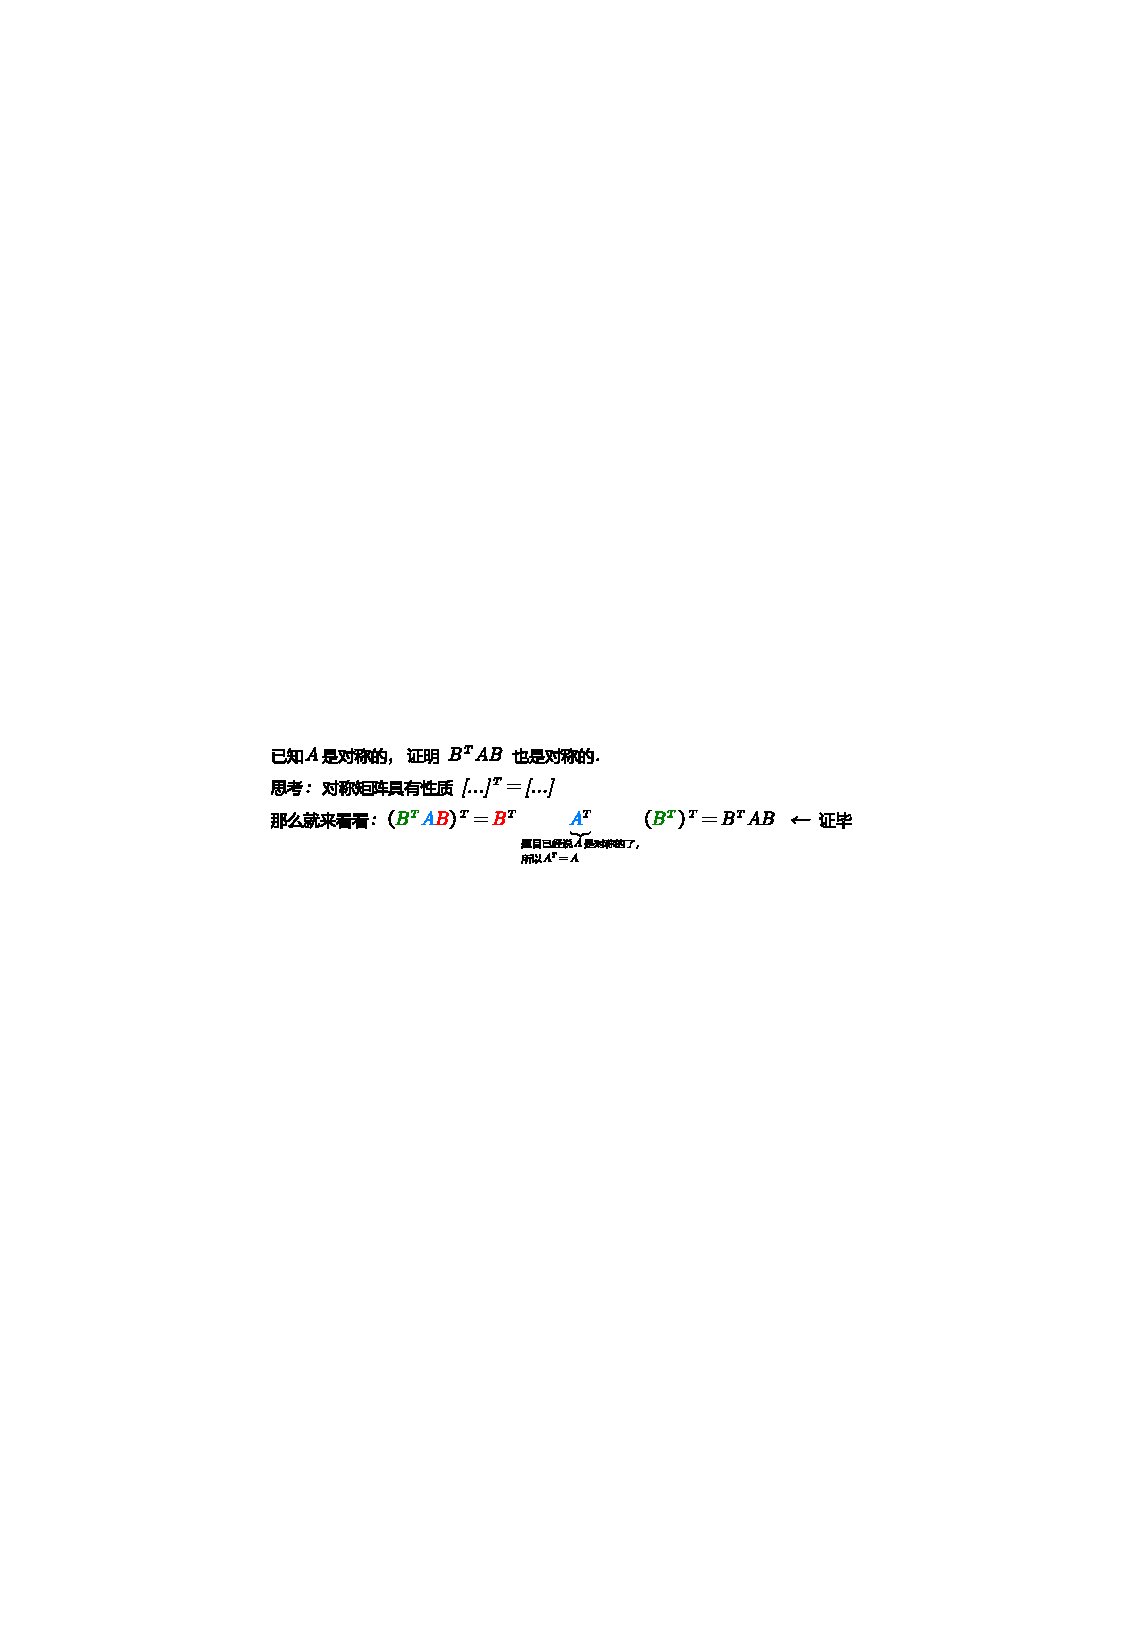
\includegraphics[width=0.8\textwidth]{img/0022.pdf}
\end{myEnvSample}





A,B 是同阶的``对称矩阵", 则有性质: 

\subsubsection{性质: $\left( A+B \right) ^T=A^T+B^T=A+B$ }

$
\left( A+B \right) ^T=\underset{A^T=A}{\underbrace{A^T}}+\underset{B^T=B}{\underbrace{B^T}}=A+B
$


\subsubsection{性质: $\left( A-B \right) ^T=A^T-B^T=A-B$ }


\subsubsection{性质: $\left( kA \right) ^T=k\cdot A^T=kA$ }

$
\left( kA \right) ^T=k\cdot \underset{A^T=A}{\underbrace{A^T}}=kA
$


\subsubsection{性质: $\left( AB \right) ^T=B^TA^T=BA\ne AB$ }

$
\left( AB \right) ^T=\underset{B^T=B.}{\underbrace{B^T}}\underset{A^T=A}{\underbrace{A^T}}=BA\ne AB
$


\subsubsection{定理: 两个对称矩阵A,B 相乘后, 新矩阵AB 一般就不再是对称的了. 除非A,B 是可交换矩阵, 型矩阵AB 才是对称的.}

即: 对称矩阵A, B, 只有在它们是``可交换矩阵"的前提下, 它们的乘积A×B, 才也是``对称矩阵". \\


\hrule


\subsection{反对称矩阵 : 有 $A^T = - A$}

反对称矩阵 Skew-symmetric matrix : 主对角线上的元素全为零,主对角线两侧对称的元素, 反号(即互为相反数). 即 $a_{ij}= -a_{ij}$ \\

如: \\
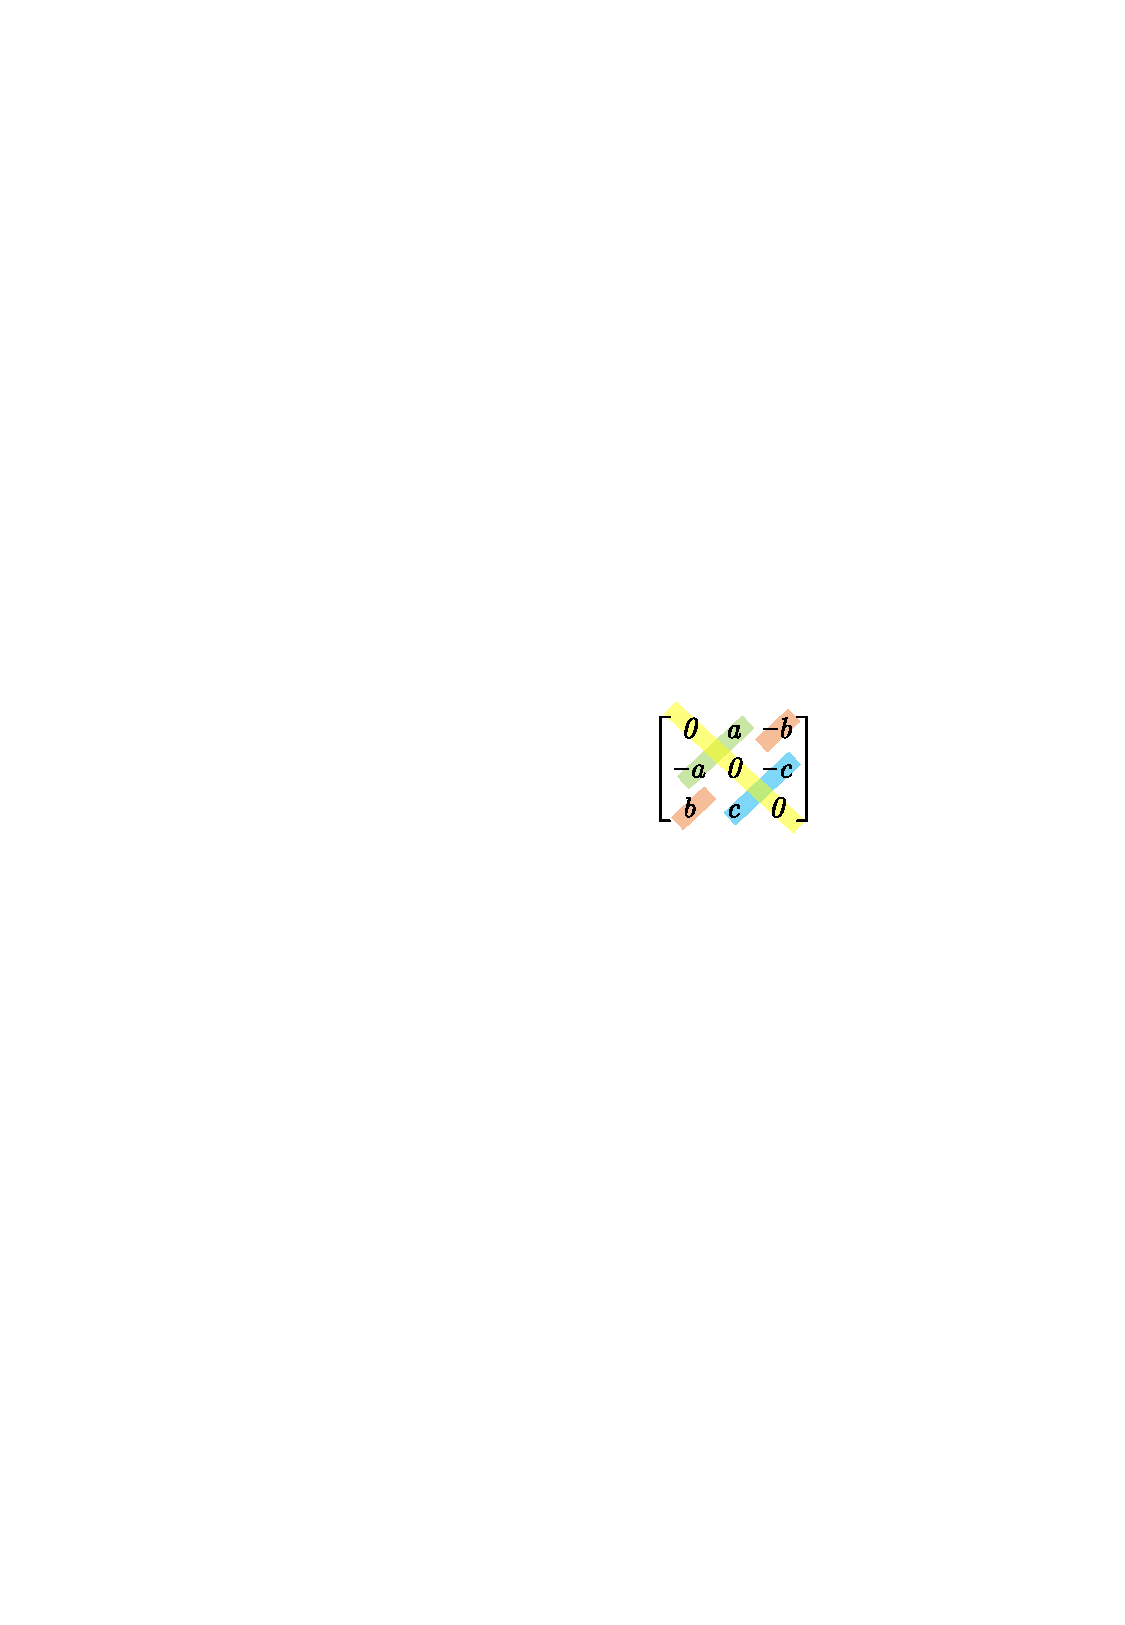
\includegraphics[width=0.15\textwidth]{img/0023.pdf} \\

为什么它主对角线上的元素都是0呢? 因为根据``反对称矩阵"的性质: $a_{ii}= -a_{ii}$, 则就 $2a_{ii}=0$, 所以就有 $a_{ii}=0$ 了. \\

反对称矩阵, 有性质: $A^T = - A$.\\


\hrule




\section{方阵的行列式}

只需把矩阵的中括号, 改成行列式的两条竖线, 就得到了``方阵的行列式". \\
如: 矩阵$
A=\left[ \begin{matrix}
	1&		1&		1\\
	2&		2&		2\\
	3&		3&		3\\
\end{matrix} \right] 
$, 其行列式就是: 
$
|A|=\left| \begin{matrix}
	1&		1&		1\\
	2&		2&		2\\
	3&		3&		3\\
\end{matrix} \right|
$\\

行列式和矩阵有什么关系? 其实, 行列式只是矩阵的一个``属性"而已. \\
矩阵有很多属性, 包括: 特征值, 特征向量, 行列式, 等等. \\



\subsection{``方阵的行列式"的性质}

\subsubsection{性质: $|A^T|=|A|$}

\subsubsection{  \ding{72} 性质: $|kA|=k^n|A|$}

\subsubsection{性质: $|AB|=|A| \cdot |B|$ ← A,B 是同阶方阵}

因此,$|ABC|=|A|\cdot |B|\cdot |C|$\\

\begin{myEnvSample}
A是5阶方阵, 且|A|=3. 求:  \\
$
\ |-A|=|-1\cdot A|=-1^5\underset{=3}{\underbrace{|A|}}=-3
$\\
$
|2A^T|=2^5\underset{=|A|=3}{\underbrace{|A^T|}}=2^5\cdot 3=96
$\\
$
\left| \underset{=3}{\underbrace{\left| A \right|}}A \right|=3^5\underset{=3}{\underbrace{|A|}}=3^6
$\\

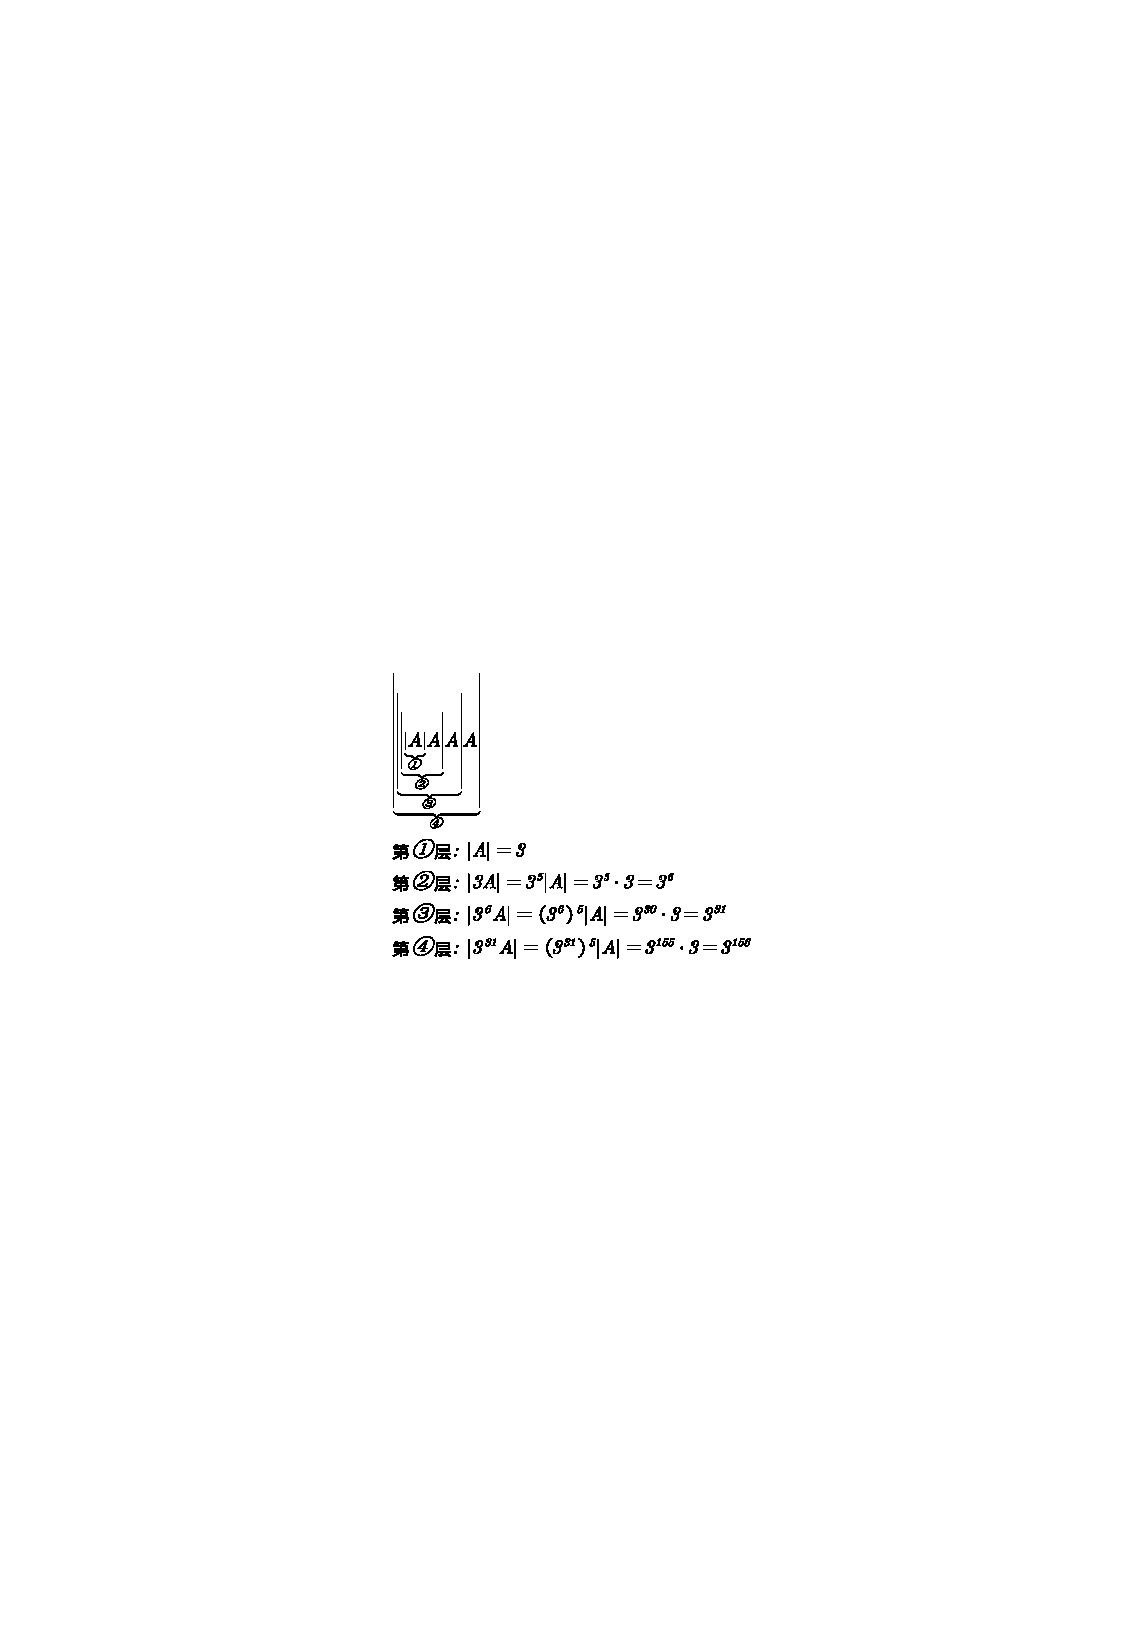
\includegraphics[width=0.55\textwidth]{img/0024.pdf}
\end{myEnvSample}



~\\
\hrule
~\\


\section{伴随矩阵  $A^*$}


\textbf{只有方阵, 才有伴随矩阵} Adjugate matrix. 并且任何方阵, 都有伴随矩阵.

如: $A=\left[ \begin{matrix}
	1&		1&		1\\
	\hline
	2&		1&		3\\
	\hline
	1&		1&		4\\
\end{matrix} \right] $ , 它的伴随矩阵 $A^*$ 是什么? \\

第1步: 先求出每个元素的``代数余子式": \\
$
A_{ij}=\left[ \begin{matrix}
	A_{11}=1&		A_{12}=-5&		A_{13}=1\\
	A_{21}=-3&		A_{22}=3&		A_{23}=0\\
	A_{31}=2&		A_{32}=-1&		A_{33}=-1\\
\end{matrix} \right]
$\\

第2步: 把$ A_{ij}$ 做转置, 就能得到A的伴随矩阵 $A^*$ :\\
$
A^*=\left[ \begin{array}{c|c|c}
	1&		-3&		2\\
	-5&		3&		-1\\
	1&		0&		-1\\
\end{array} \right]
$\\

即: 按``行"求的``代数余子式", 按``列"放. \\
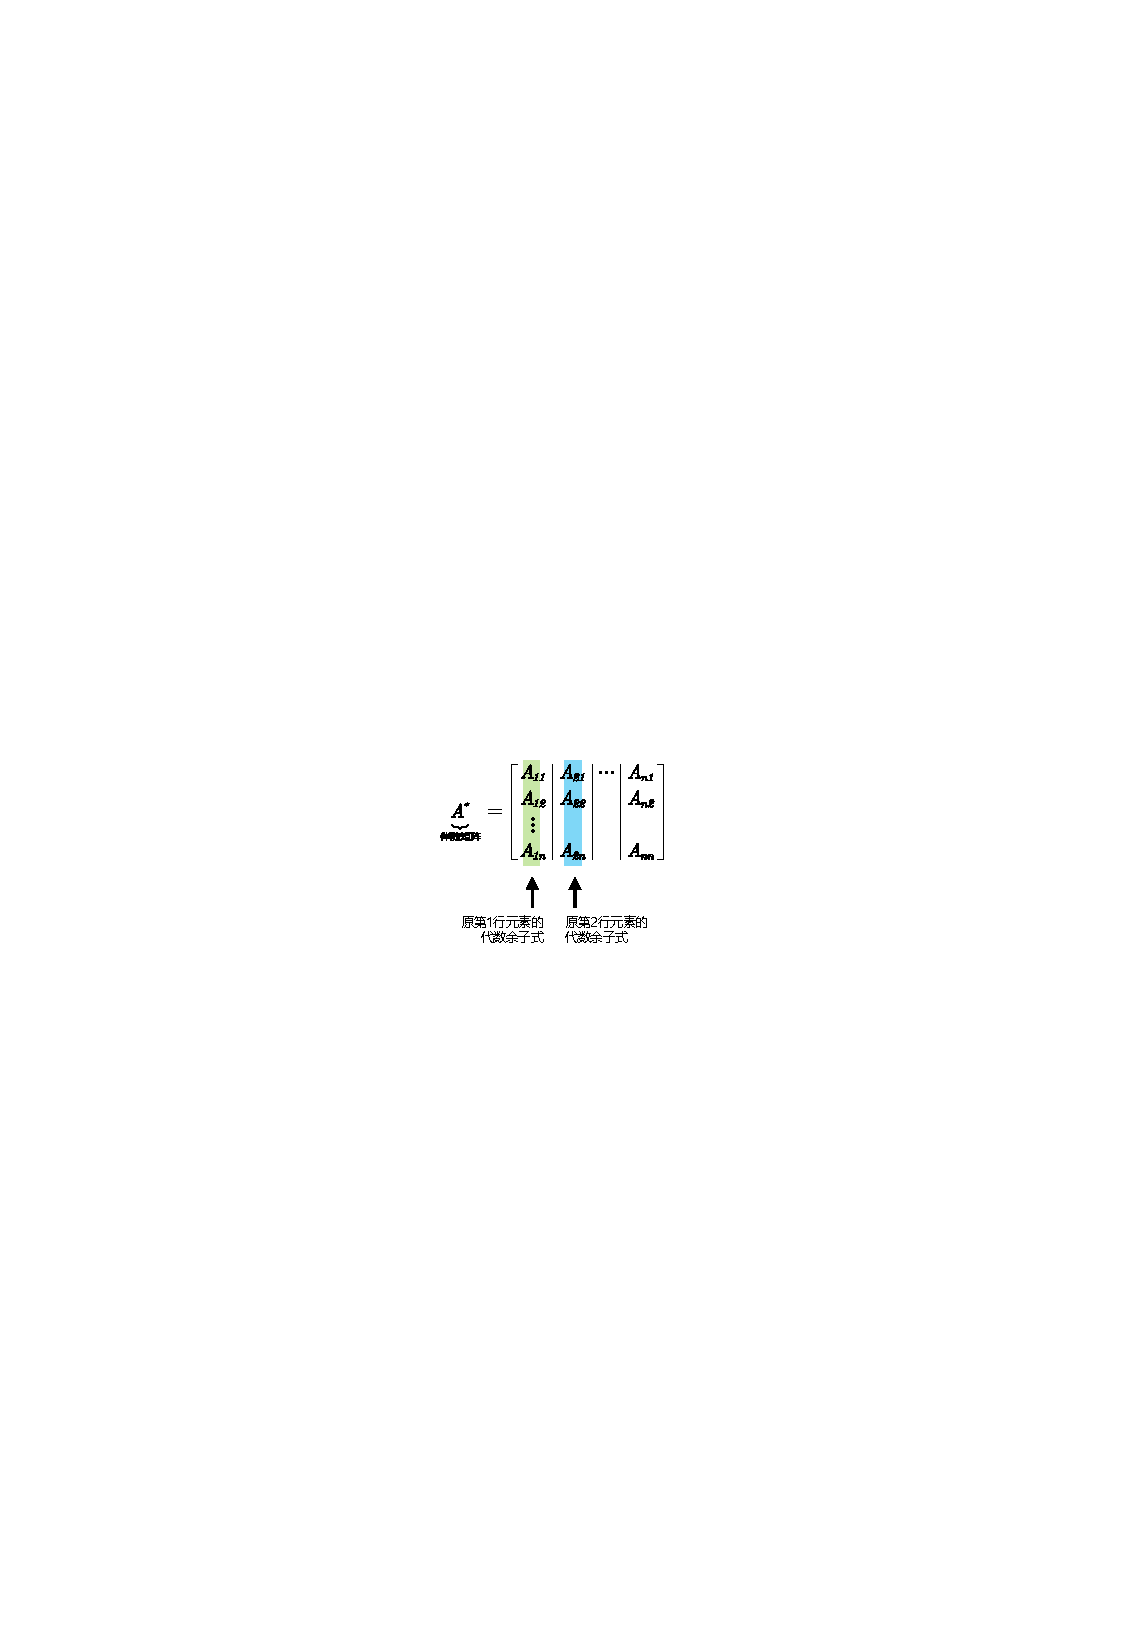
\includegraphics[width=0.35\textwidth]{img/0025.pdf}\\


【已知A, 如何求得它的伴随矩阵 $A^*$ ?】 : 
\begin{align*}
	& \text{因为}A\text{的逆阵,有这个性质:\ }A^{-1}=\frac{1}{|A|}A^*\\
	& \text{所以,\ 把分母拿到等号左边,就有:\ |}A|A^{-1}=A^*
\end{align*}

即, 只要把A的行列式, 和A的逆阵, 相乘, 就能得到 A的伴随矩阵.
即:
\begin{align*}
	\boxed{
		|A|A^{-1}=A^*
	}
\end{align*}




\begin{myEnvSample}
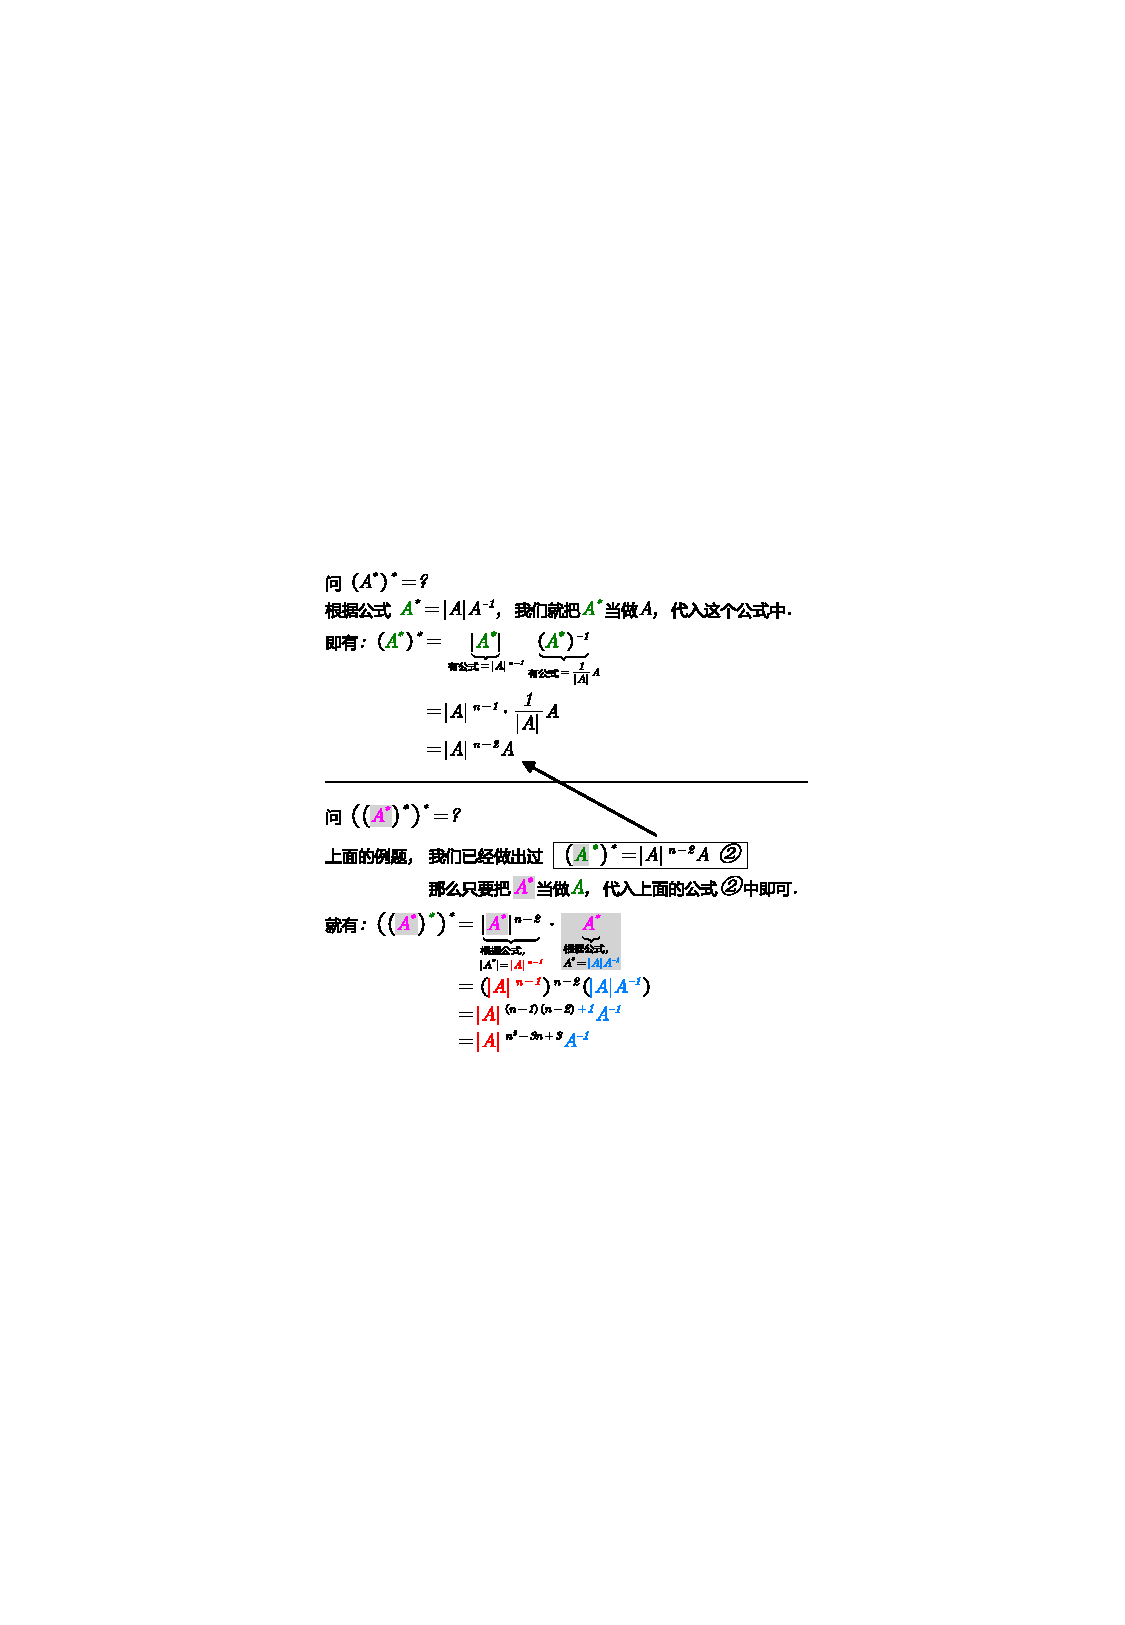
\includegraphics[width=0.7\textwidth]{img/0029.pdf}
\end{myEnvSample}



\hrule


\subsection{伴随矩阵的性质}

\subsubsection{性质: 对``任意"方阵A, 有: $A * A^{\ast} = A^{\ast} * A = |A|E$}

\begin{myEnvSample}
只有一个元素组成的方阵 $ A=[5] $, 其 $ A^*$ 是什么 ? \\

根据性质: \\
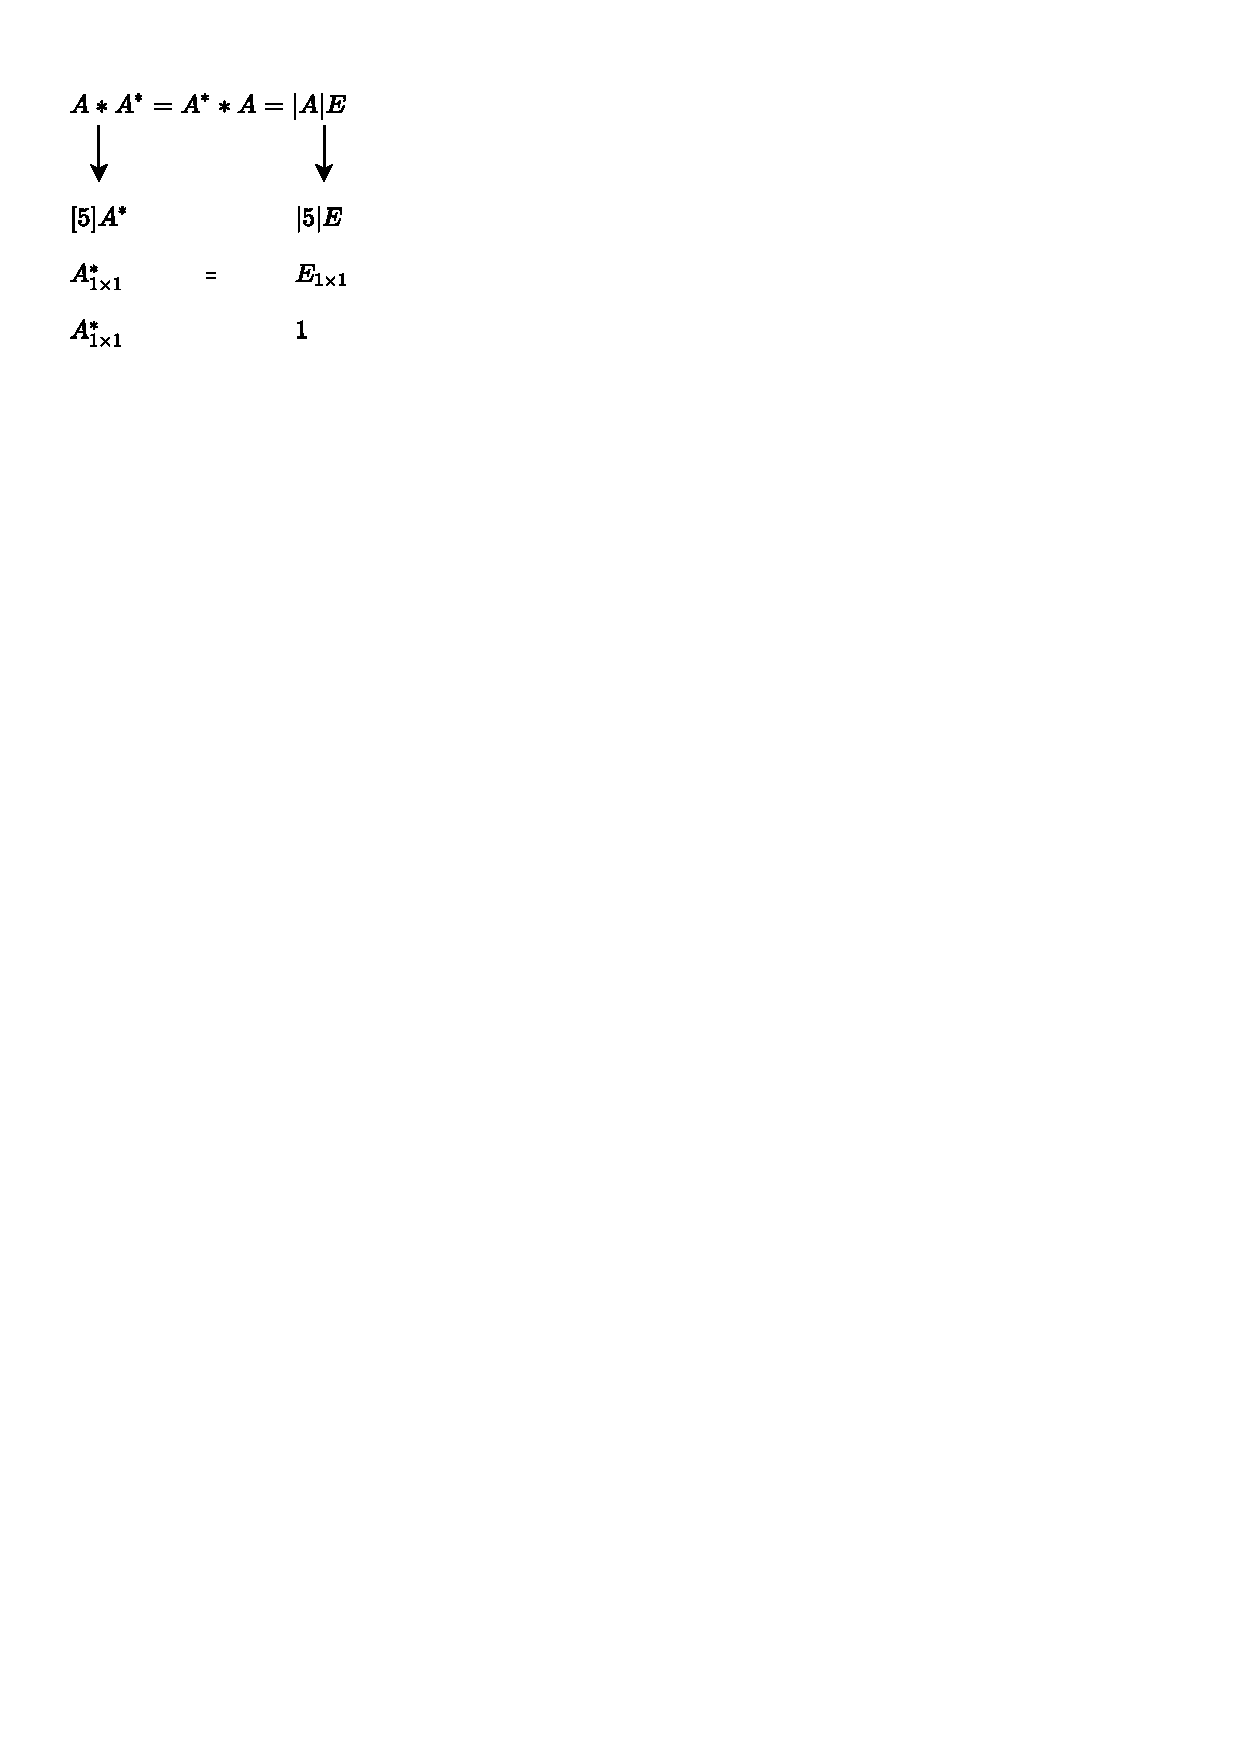
\includegraphics[width=0.3\textwidth]{img/0027.pdf}
\end{myEnvSample}




\subsubsection{性质: $|A\cdot A^*|=|A|^n\cdot |E|$ }

\subsubsection{性质: $|A^*|=|A|^{n-1}$ }

证明过程如下: \\
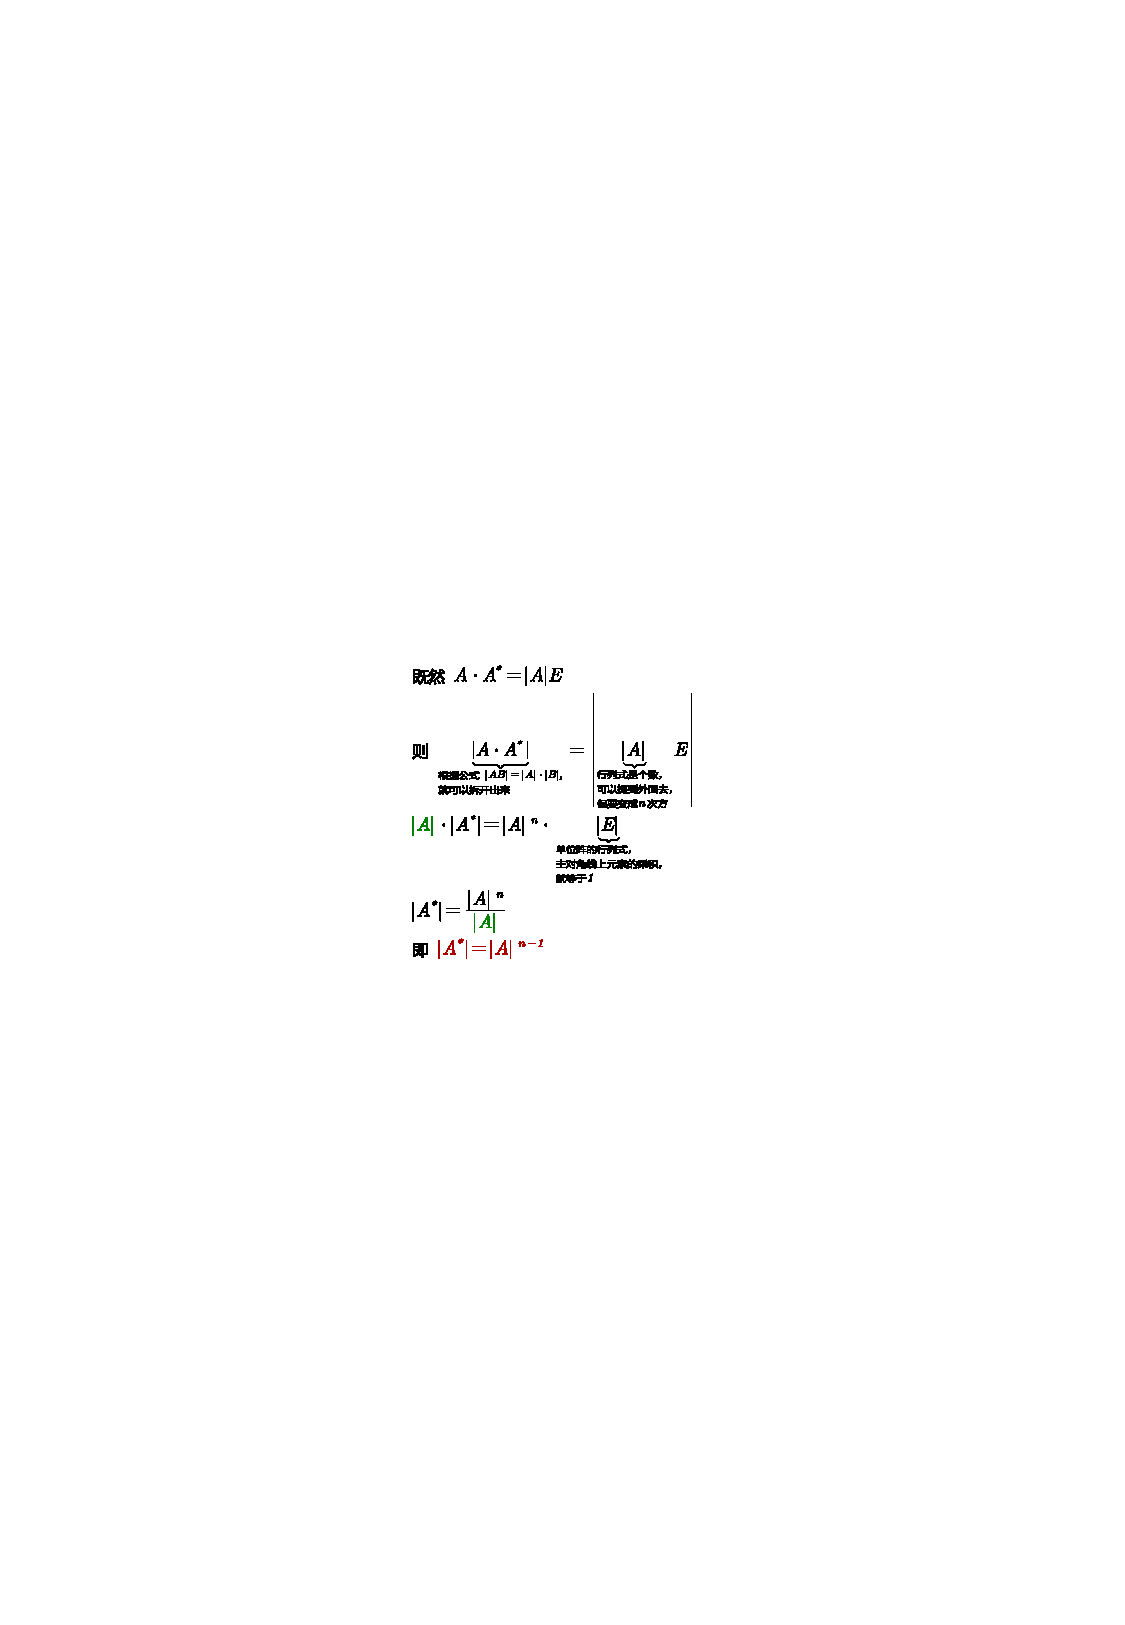
\includegraphics[width=0.4\textwidth]{img/0026.pdf}\\



\subsubsection{性质: $\left( kA^* \right) =k^{n-1}A^*$ }

\subsubsection{性质: $\left( A^T \right) ^*=\left( A^* \right) ^T$ }

\subsubsection{性质: $\left( AB \right) ^*=B^*A^*$ }



~\\
\hrule
~\\


\section{逆矩阵}

\subsection{``逆"的几何意义 → 相当于 ctrl + z 操作}

逆阵, 就相当于 ctrl + z 操作.\\

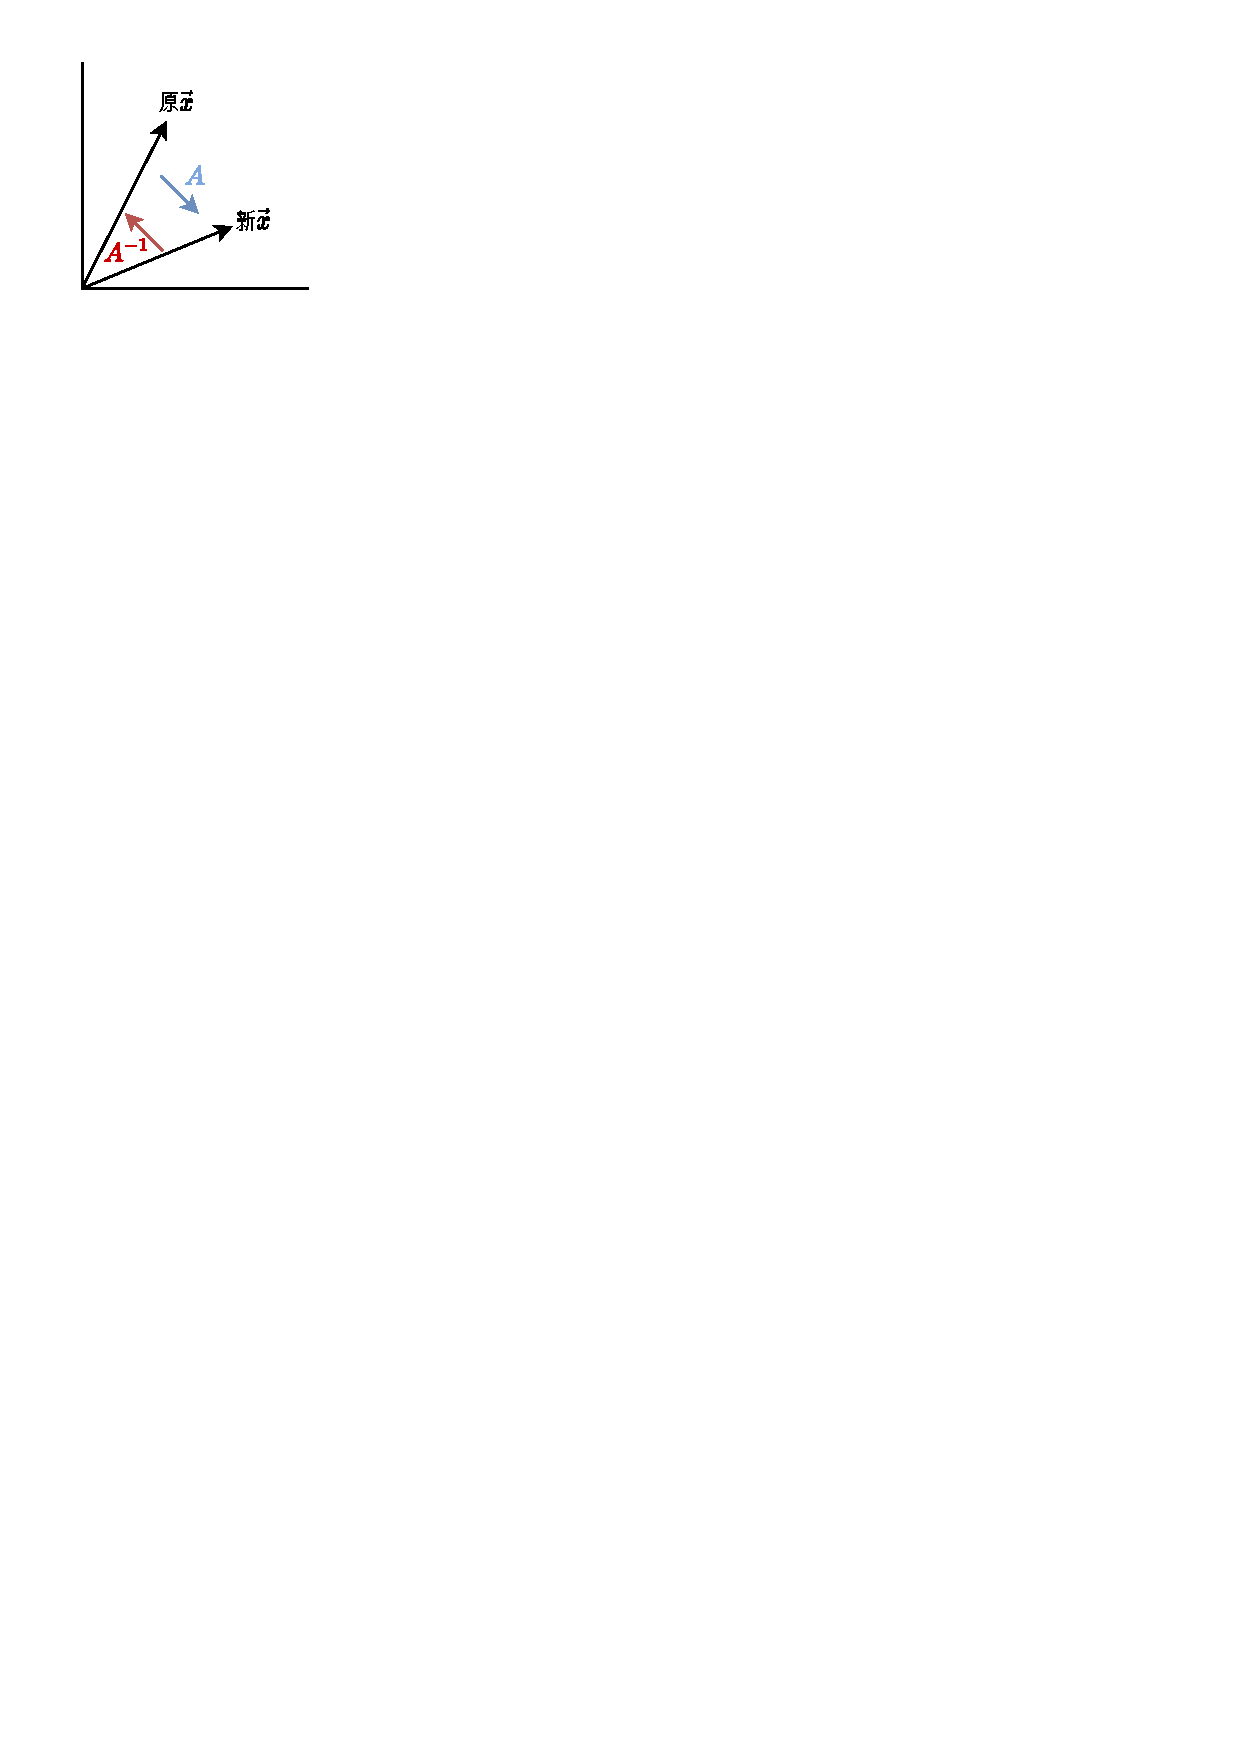
\includegraphics[width=0.2\textwidth]{img/0048.pdf}\\

→ 如果从``原像"变到``异像", 应用的是 A(新基矩阵) 变换规则; \\
→ 则从``异像"变回``原像", 可以用 $ A^{-1}$ 变换规则来实现.\\

即: 如果 A 是``顺时针旋转90度"的变换; 则  $ A^{-1}$ 就是``逆时针旋转90度"的变换, 即它能对A 做 ctrl + z 操作, 抵消掉A的影响.\\

\begin{align*}
	\underset{\text{撤销掉A变换.}}  {\underbrace{A^{-1}}}\underset{\text{做A变换}}{\underbrace{A}}\overrightarrow{x}\ =\ \overrightarrow{x}
\end{align*}

所以, 对于 $[ Ax=b$, 为了求出``原像x", 只要把等号左边的A撤销掉 (直接给它乘上一个A的逆), 就能暴露出x了, 即直接就能得到``解".

\begin{align*}
	& A\vec{x} = \vec{b} \\
	& A^{-1} \cdot A \cdot \vec{x} = A^{-1} \cdot \vec{b} \ ← \text{两边等式乘上A的逆}\\
	& \vec{x} = A^{-1}  \vec{b} \ ← \text{直接就能得到原像}\vec{x}, 即方程组的解
\end{align*}

换言之, \textbf{我们只要找到了A的逆阵, 就能利用它来计算出方程组的解. 这就是``逆阵"带给我们的作用之一. }\\

要记住一句话: 线性代数中,\textbf{矩阵不能放在分母上!} \\


~\\
\hrule
~\\


\subsection{可逆矩阵 : AB = BA = 单位阵E}


有方阵  $ A_{n \times n}$, 若存在一个 $ A_{n \times n}^{-1}$, 使得  $ A \cdot A^{-1} = A^{-1} \cdot A = E$ (类似于 $ 2 \cdot \frac{1}{2} =  \frac{1}{2} \cdot 2 $), 则称 A可逆, 且 $A^{-1} $ 就是A的逆矩阵. \\


【可逆矩阵】 invertible matrix : A,B为n阶方阵,若 \textbf{AB = BA = 单位阵E,} 则称 A为``可逆矩阵""(或``非奇异矩阵"),B为A的``逆矩阵",\textbf{记为 $A^{-1}=B$. ← 意思即: A的逆矩阵, 是B.} \\ 

注意: \\
1.并非所有方阵均可逆. \\
比如零矩阵, OA = AO = O, 它就不满足``可逆矩阵"的要求 AB = BA = E 了. 所以零矩阵不可逆.\\

2.\textbf{若A为``可逆矩阵",则A的``逆矩阵"是唯一的.}\\




\begin{myEnvSample}
	已知 A+B = AB , 验证:  A-E 是可逆的. 
	\begin{align*}
	& \text{既然}A+B=AB\\
& \text{则\ }AB-A-B=O\text{零矩阵}\\
& AB-A-B+E=O+E\ ←\text{两边同时加上单位阵}E\\
& \underset{=(A-E)B}{\underbrace{AB-B}}-A+E=E\\
& (A-E)B-\left( A-E \right) =E\ ←\text{等号左边,\ 提取}\left( A-E \right)\\
& \left( A-E \right) \underset{\text{这个,\ 就是}\left( A-E \right) \text{的逆矩阵了}}{\underbrace{\left( B-E \right) }}=E\\
& \text{即:\ }\left( A-E \right) ^{-1}=B-E
\end{align*}
\end{myEnvSample}



~\\
\hrule
~\\

\subsubsection{如何判断一个矩阵是否可逆? A可逆的充要条件是: $|A| \ne 0$. 并且A的逆矩阵就是: $	A^{-1}=\frac{1}{|A|}A^*	$}



【如何判断一个矩阵是否可逆?】: \\
\textbf{判断方法就是: 只要它的行列式 |A| 不等于0, 它就是可逆的.}\\
这种行列式的值不为0 的方阵, 也叫``非奇异 /非退化 /满秩"的.\\

因为\textbf{行列式的值, 就是它们向量所组成的``平行四边形"的面积. 若 面积=0 了, 说明原坐标系空间被``变换"成零维了, 被降维压缩了.} 高维信息全部丢失. \textbf{而``逆矩阵"是实现 ctrl + z 作用的, 显然零维物体就无法还原成高维物体了.} 所以 ctrl + z 就不可做了. 即不存在你操作, 不存在 $ A^{-1}$.\\

即: 当行列式值=0 时, 就说明新基矩阵A 将坐标轴空间, 变换压缩到了更低的维度上(比如一条直线上). \textbf{此时就没有``逆变换", 因为你不能将一条线``解压缩"为一个平面. 至少这不是一个函数能做到的. 如果你硬要还原, 这会导致多重映射的问题. 但是函数(包括反函数)只能将一个输入变换为一个输出.} -- that would require transforming(v.) each individual vectors /into a whole line full of vectors. but functions can only take a single input /to a single output. \\

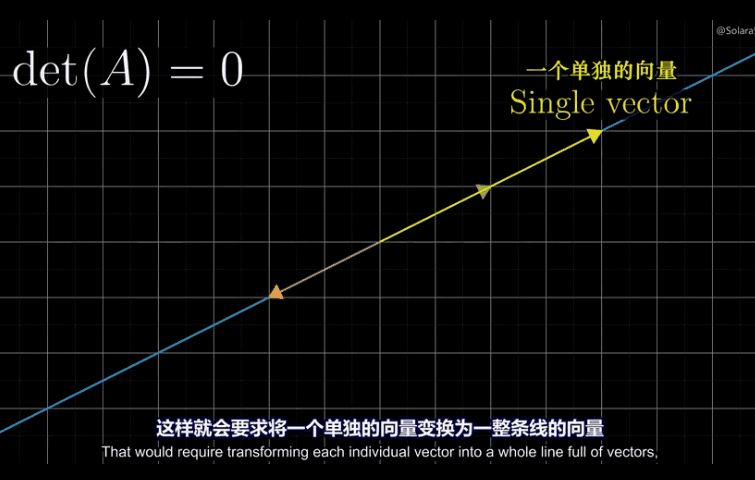
\includegraphics[width=0.4\textwidth]{img/0049.png} 
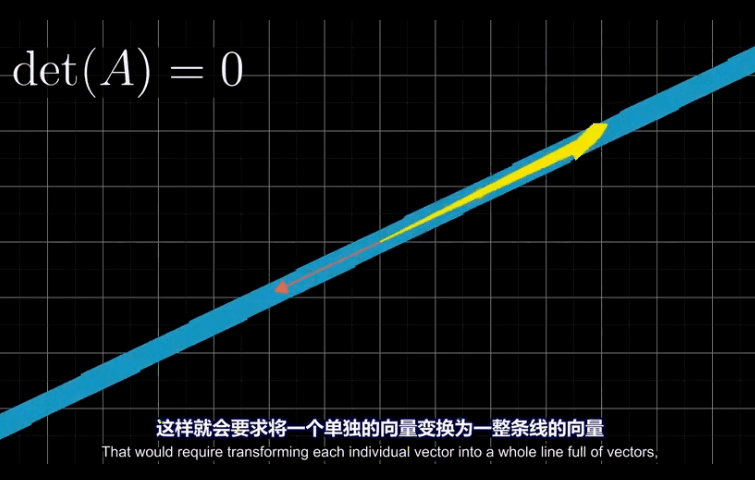
\includegraphics[width=0.4\textwidth]{img/0050.png} \\
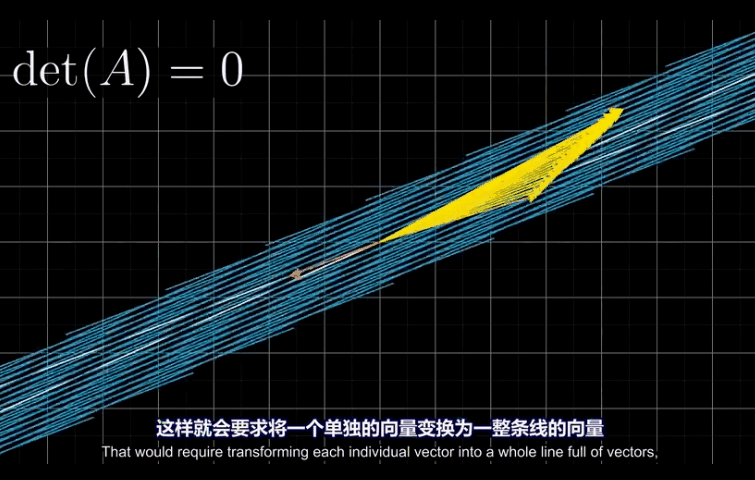
\includegraphics[width=0.4\textwidth]{img/0051.png} 
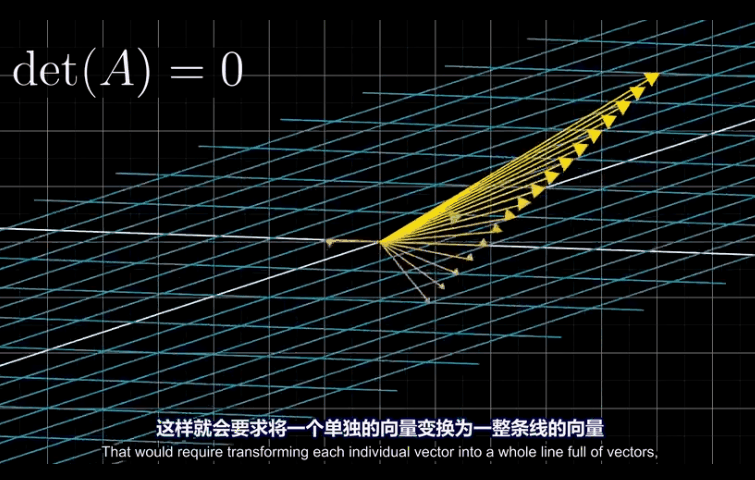
\includegraphics[width=0.4\textwidth]{img/0052.png} \\
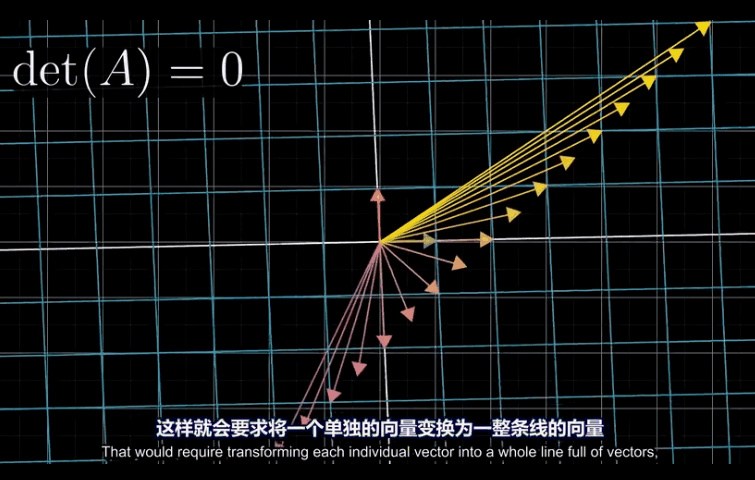
\includegraphics[width=0.4\textwidth]{img/0053.png} \\


类似的, 对于三个方程和三个未知数, 如果变换是将三维空间, 压缩为一个平面, 甚至是一条直线, 或一个点, 那么它也没有逆变换.\\

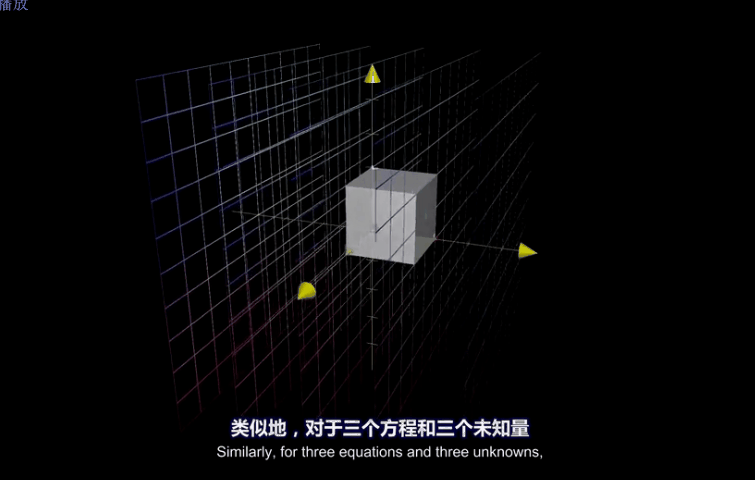
\includegraphics[width=0.4\textwidth]{img/0054.png} 
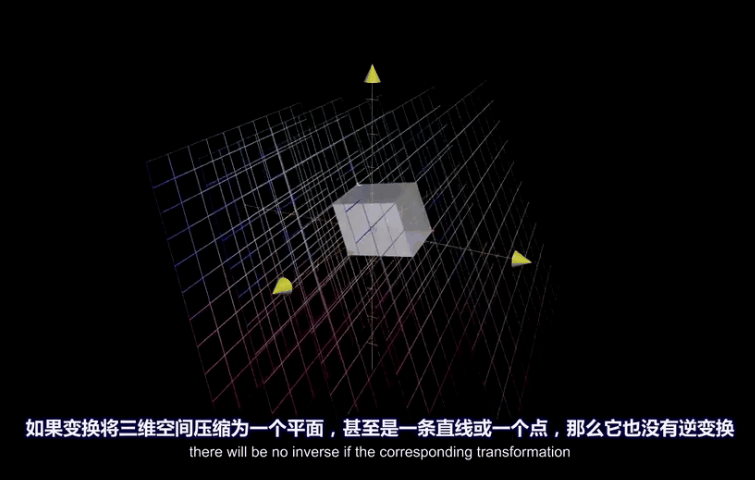
\includegraphics[width=0.4\textwidth]{img/0055.png} \\
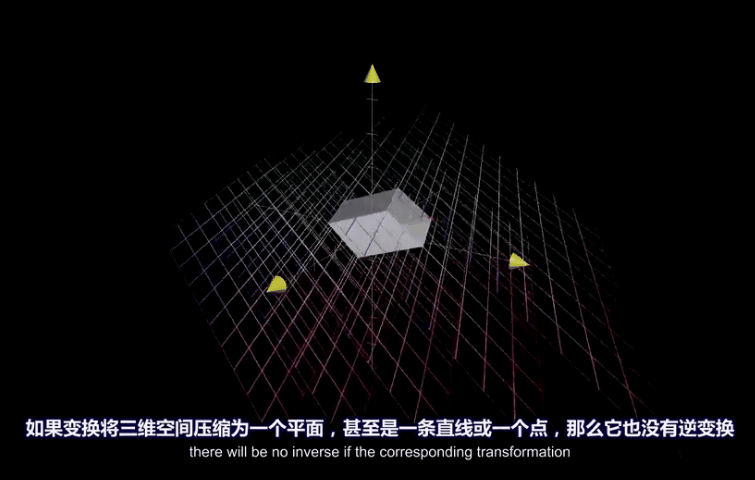
\includegraphics[width=0.4\textwidth]{img/0056.png} 
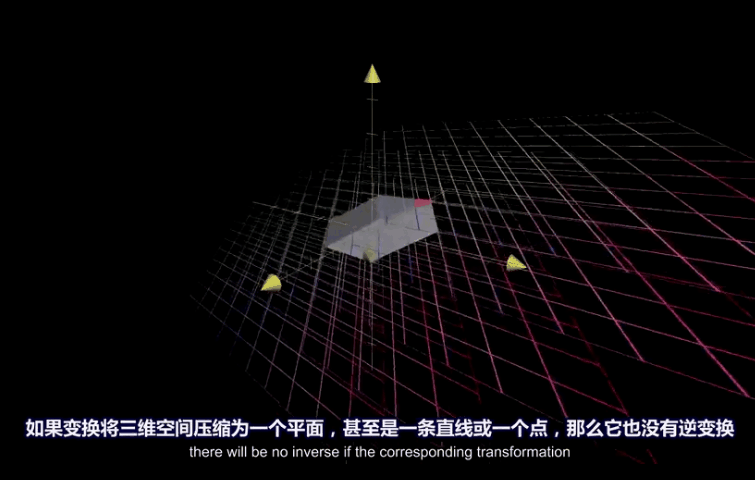
\includegraphics[width=0.4\textwidth]{img/0057.png} \\
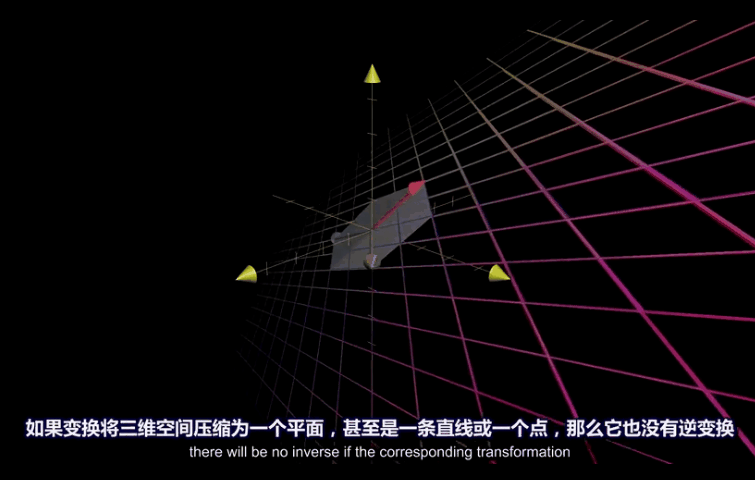
\includegraphics[width=0.4\textwidth]{img/0058.png} \\

它们都对应``行列式值为零"的情况, 因为此时, 所有区域都被压缩到零体积. \\

但即便不存在逆变换, ``解"仍然可能存在. it's still possible that a solution exists /even when there is no inverse. \\
比如说, 一个变换, 将``原坐标系空间"压缩为一条直线, 如果``原像$\vec{x}$" 恰好就处在这条直线上, 那降维后, 你仍然没有失去它. 即, 解(即$\vec{x}$) 依然存在. 但如果``原像"是处在这条直线外面的, 那降维后, 你就失去它了.\\

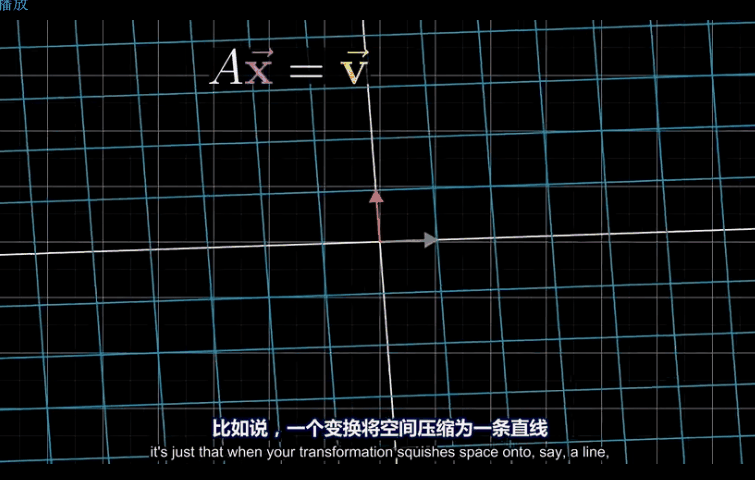
\includegraphics[width=0.4\textwidth]{img/0059.png} 
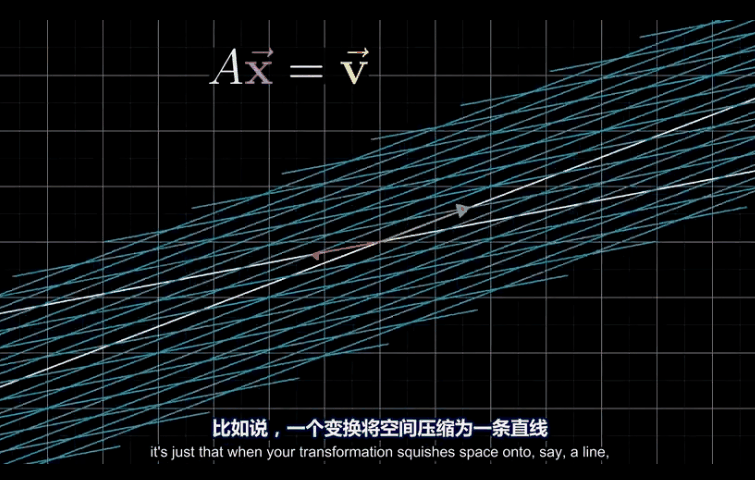
\includegraphics[width=0.4\textwidth]{img/0060.png} \\
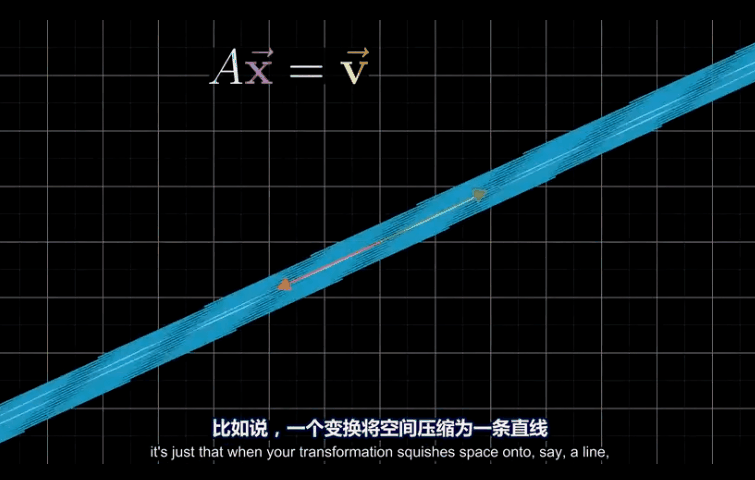
\includegraphics[width=0.4\textwidth]{img/0061.png} 
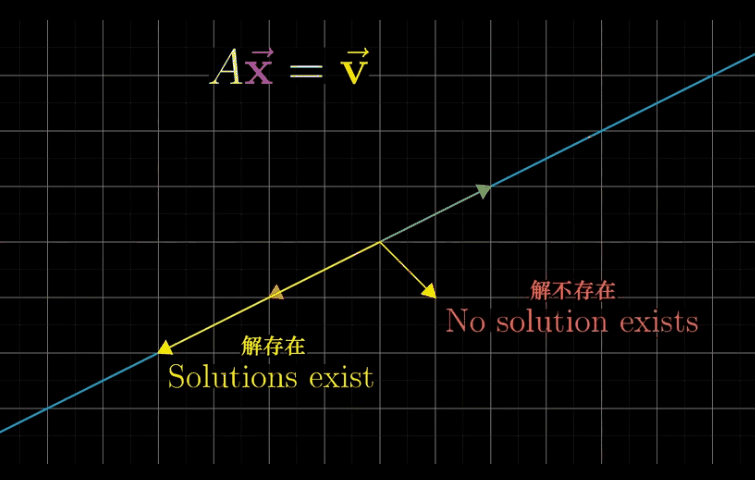
\includegraphics[width=0.4\textwidth]{img/0062.png} \\








【逆矩阵的公式】: \\
如果一个矩阵是可逆的, 它的逆矩阵是什么呢? 公式就是: 
\begin{align*}
	\boxed{
			A^{-1}=\frac{1}{|A|}A^*
	}
\end{align*}


\begin{myEnvSample}
``A的逆矩阵"公式, 其证明过程是: 
\begin{align*}
	&\text{因为对任何方阵,\ 都有:} AA^*=A^*A=|A|E\  \\
&\text{我们有|}A|\ne 0\text{这个前提条件,\ 那么就把}\text{上式两边同时除以\ |}A|\\
&\text{即:\ }A\frac{1}{|A|}A^*=A^*\frac{1}{|A|}A=|A|\frac{1}{|A|}E\\
&A\underset{\text{把这块看成}B}{\underbrace{\left( \frac{1}{|A|}A^* \right) }}=\underset{\text{把这块看成}B}{\underbrace{\left( A^*\frac{1}{|A|} \right) }}A=E\ ←\text{这不就是满足}AB=BA=E,\ \text{这个可逆矩阵的定义吗?}\\
&\text{所以,\ }A\text{的逆矩阵,\ 就是}\frac{1}{|A|}A^*
\end{align*}
\end{myEnvSample}


\subsubsection{推论: A,B是n阶方阵, 只要我们知道一个条件: AB=E, 或BA=E, 我们就能得出结论: A可逆, 并且$A^{-1}=B$ }



~\\
\hrule
~\\

\subsection{求``逆矩阵"的方法}


\subsubsection{用``伴随矩阵法"(不推荐用), 来求逆矩阵 : 利用A的逆矩阵公式, 来求A的逆矩阵. 即:  $	A^{-1}=\frac{1}{|A|}A^*	$ }

\begin{align*}
	& \because A^{\ast} = |A| A^{-1} \\
	& \therefore \frac{A^{\ast}}{|A| } = A^{-1} \\
	&
	\boxed{
		A^{-1}  =  \frac{1}{|A| } A^{\ast}
	}
\end{align*}

不过, 实际中, 该求逆方法很少用, 因为要先求$A^*$, 计算量太大. \\




\subsubsection{用``初等变换法", 来求逆矩阵 (常用): $	[ A,E] →\text{初等行变换} →[E,A^{-1}]	$ }
	
	比如, 要求A的逆阵, 可以先写这样一个矩阵: [A|E],  把它左边的A, 先变换成E, 则它右边原先的E, 就会变成A的逆阵了. 我们就能得到 $A^{-1}$ 了. \\
	
	
	即: 只做``初等行变换": $
	\left[ A,E \right] \underrightarrow{\text{初等行变换}}[E,A^{-1}]
	$ ← 当``左边的A"变成``右边的E"时, ``左边的E"也就能变成了``右边的$A^{-1}$". 我们就得到了$A^{-1}$. \\
	
	\begin{myEnvSample}
		\begin{align*}
& \text{已知} A=\left[ \begin{matrix}
	1&		0&		1\\
	2&		1&		0\\
	-3&		2&		-5\\
\end{matrix} \right]  \\
& \text{把A和E拼在一起, 构成一个矩阵} \\
& [A|E]=\left[ \begin{array}{ccc|ccc}
	1&		0&		1&		1&		&		\\
	2&		1&		0&		&		1&		\\
	-3&		2&		-5&		&		&		1\\
\end{array} \right] \\
& \text{做初等行变换, 把竖线左边原先的A, 化成单位阵E:} \\
& AE=\left[ \begin{array}{ccc|ccc}
	1&		&		&		-\frac{5}{2}&		1&		-\frac{1}{2}\\
	&		1&		&		5&		-1&		1\\
	&		&		1&		\frac{7}{2}&		-1&		\frac{1}{2}\\
\end{array} \right]
		\end{align*}
	
		现在, 竖线右边的部分, 就是 $A^{-1}$了.
	\end{myEnvSample}
	
	
做法总结:\\

1. 先搞第1列, 再第2列, 第3列... \\
2. \textbf{``第1列"处理完后, ``第1行"(注意是行!) 就不再主动参与后面的运算. 即不再用 line1 去消下面的行.} 但能用下面的行, 去消 line1上的元素到0.\\
3. 变换时, 矩阵与矩阵之间, 不能写等号, 要写箭头(→), 即: [] -> [] -> [].\\
4. 只做``行变换", 而绝不做能``列变换".\\
5. \textbf{如果最后发现 [A|E]的左边, 化不成单位阵E时, 就说明A不可逆.}\\
	
	
	\begin{myEnvSample}
关于上面第5点, 比如, 对于这个矩阵: 
	$A=\left[ \begin{matrix}
		1&		2&		3\\
		2&		4&		9\\
		4&		8&		18\\
	\end{matrix} \right]$\\
	经过行变换, 你发现 [A|E]只能变成:
	$[A|E]=\left[ \begin{array}{ccc|ccc}
		1&		2&		3&		1&		&		\\
		0&		0&		3&		-2&		1&		\\
		0&		0&		0&		&		-2&		1\\
	\end{array} \right]$\\
	
你发现竖线左边, 化不成E, 就说明这个A不可逆. \\
其实, 你发现, 左边这个行列式的值 = 0. 即 |A|=0, 也说明了A不可逆.
	\end{myEnvSample}

~\\
\hrule
~\\


\subsection{逆矩阵的性质}


\subsubsection{若A可逆, 则$A^{-1}$ 也可逆, 并且有 $\left( A^{-1} \right) ^{-1}=A$ }

证明过程: 
\begin{align*}
		& \text{因为根据}“\text{逆矩阵}”\text{的定义:\ 只要}AB=E,\ \text{则}A^{-1}=B\\
	& \text{那么我们就反过来看看,\ }A^{-1}A\text{是否}=E,\ \text{如果等于,则就证明了}A^{-1}=A\text{了}.\\
	& A^{-1}A\text{肯定}=E\text{了}.
\end{align*}

~\\
\hrule
~\\

\subsubsection{若A,B 均可逆, 则有: AB也可逆, 并且有: $\left( AB \right) ^{-1}=B^{-1}A^{-1}$}

\begin{myEnvSample}
证明过程: 
\begin{align*}
	& \text{既然(AB)可逆, 就有:} \\
	& (AB)(AB)^{-1} = E \\
	& (AB)(B^{-1} A^{-1}) = E \ ← \text{这一步, 就已经证明了 AB 的逆阵是}  B^{-1} A^{-1}
\end{align*}
\end{myEnvSample}



所以同样: $
\left( ABCD \right) ^{-1}=D^{-1}C^{-1}B^{-1}A^{-1}  
$  ← 注意等号右边, 顺序是倒过来的. 这个和转置公式($\left( AB \right) ^T=B^TA^T$ )很像. 

~\\
\hrule
~\\

\subsubsection{若A可逆, 则$A^T$ 也可逆. 并且有: $\left( A^T \right) ^{-1}=\left( A^{-1} \right) ^T$ ← 转置的逆 = 逆的转置}

~\\
\hrule
~\\

\subsubsection{$k\ne 0,\ \text{则}\left( kA \right) ^{-1}=\frac{1}{k}A^{-1}$}

证明过程:
\begin{align*}
		& \text{只要来看看\ }kA\cdot \frac{1}{k}A^{-1}\ \text{是否}=E\text{就行了,它们就互为逆矩阵}.\\
	& kA\cdot \frac{1}{k}A^{-1}=k\frac{1}{k}\cdot AA^{-1}=1\cdot E=E\ ←\text{的确等于}E.
\end{align*}

你发现, $\frac{1}{k} $ 这个数, 其实就是对k的变换, 能做 ctrl + z 的操作.

~\\
\hrule
~\\

\subsubsection{性质: $|A^{-1}|=|A|^{-1}$}

若A可逆, 则$ |A^{-1}| = |A|^{-1}$, 即: 逆的行列式 = 行列式的逆.

~\\
\hrule
~\\

\subsubsection{性质: 若A可逆, 则 $A^{*}$(即伴随矩阵)也可逆. 并且 $(A^{*})^{-1} =  \frac{1}{|A| } A$ }


证明过程:
\begin{align*}
		& A^*\text{有这个性质\ }AA^*=|A|E\\
	& \text{那么两边同时除以|}A|,\ \text{即:\ }\frac{1}{|A|}AA^*=\frac{1}{|A|}|A|E\\
	& \text{即\ }\left( \frac{1}{|A|}A \right) A^*=E\ ←\ \text{所以一看就知道,}A^*\text{的逆矩阵,\ 就是}\frac{1}{|A|}A
\end{align*}

~\\
\hrule
~\\

\subsubsection{性质: $\left( A^{-1} \right) ^*=\left( A^* \right) ^{-1}$ }

A可逆时, $A^{*}$ 也可逆.

	
~\\
\hrule
~\\	
	

\subsubsection{单位阵E是可逆的.  $E^{-1} = E $}

\subsubsection{零矩阵不可逆, 因为其行列式=0了. 只有行列式不等于0的, 才有逆.}


	
	
~\\
\hrule
~\\
	
	\section{矩阵方阵}

	
	\begin{myEnvSample}
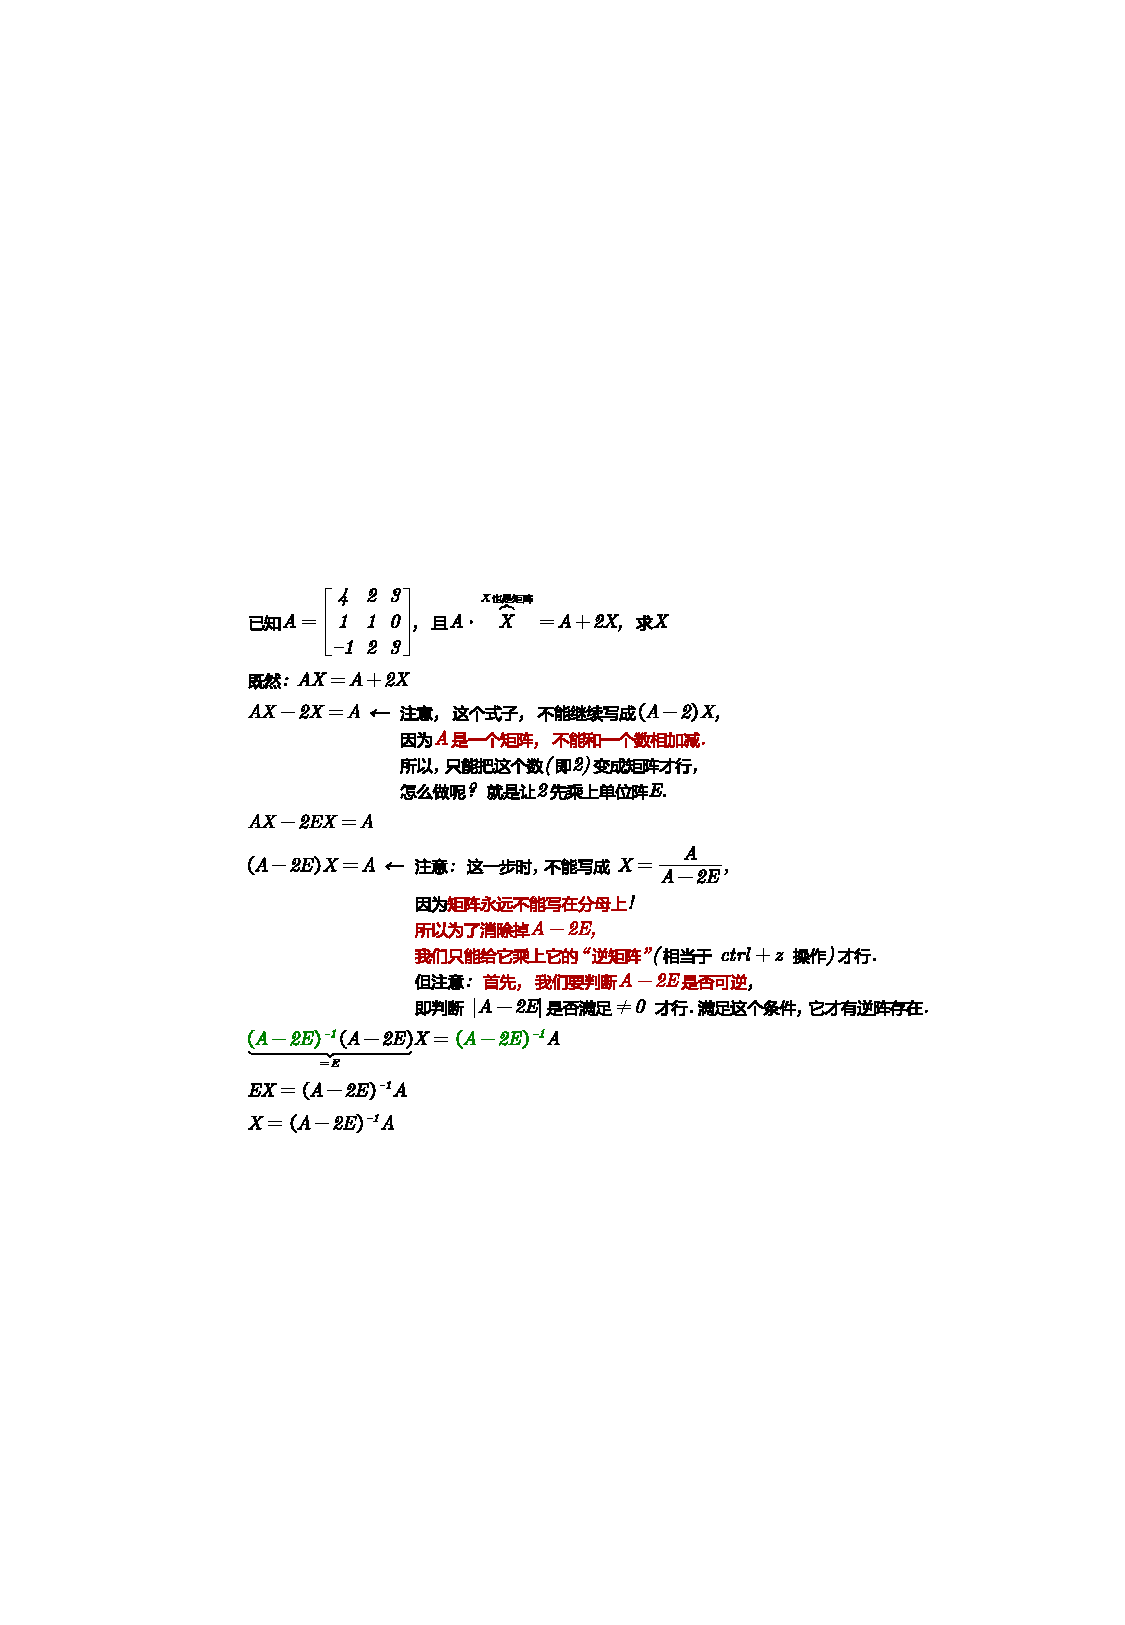
\includegraphics[width=0.9\textwidth]{img/0028.pdf}\\
	\end{myEnvSample}


~\\
\hrule
~\\

\section{分块矩阵}

\subsection{标准形}

标准形, 形如: \\
$
\left[ \begin{matrix}
	1&		&		&		&		&		\\
	&		\ddots&		&		&		&		\\
	&		&		1&		&		&		\\
	&		&		&		0&		&		\\
	&		&		&		&		\ddots&		\\
	&		&		&		&		&		0\\
\end{matrix} \right]_{m×n} 
$ \\

即: 从左上角开始的一串1, 不能断. 其余的地方全是0.\\
注意: 标准形, 不一定是方阵. \\

如: \\
$
\left[ \begin{matrix}
	1&		&		\\
	&		1&		\\
	&		&		0\\
\end{matrix} \right] 
$ ← 这个\underline{是}标准形. \\

$
\left[ \begin{matrix}
	1&		&		&		\\
	&		1&		&		\\
	&		&		1&		0\\
\end{matrix} \right] 
$ ← 这个也\underline{是}标准形. 哪怕它没有0. \\

$
\left[ \begin{matrix}
	1&		&		&		\\
	&		1&		&		\\
	&		&		1&		\\
	&		&		&		1\\
\end{matrix} \right] 
$ ← 这个也\underline{是}标准形. 没有0也是. \\

$
\left[ \begin{matrix}
	0&		&		\\
	&		1&		\\
	&		&		1\\
\end{matrix} \right] 
$ ← 这个\underline{不是}标准形.  \\

$
\left[ \begin{matrix}
	1&		&		&		\\
	&		1&		&		\\
	&		&		0&		\\
	&		&		&		1\\
\end{matrix} \right] 
$ ← 这个\underline{不是}标准形. 因为1被断开了. \\


$
\left[ \begin{matrix}
	0&		&		\\
	&		0&		\\
	&		&		0\\
\end{matrix} \right] 
$ ← 这个\underline{是}标准形. 完全没有1也是.\\


对``标准形", 我们可以对它做分块.\\
$
\left[ \begin{array} {ccc|ccc}
	1&		&		&		&		&		\\
	&		\ddots&		&		&		&		\\
	&		&		1&		&		&		\\
	\hline
	&		&		&		0&		&		\\
	&		&		&		&		\ddots&		\\
	&		&		&		&		&		0\\
\end{array} \right] 
=\left[ \begin{matrix}
	E_r&		O_{r\cdot \left( n-r \right)}\\
	O_{\left( m-r \right) \cdot r}&		O_{\left( m-r \right) \cdot \left( n-r \right)}\\
\end{matrix} \right] 
$\\

\hrule

\subsection{分块矩阵的 ``加法"}

$
\left[ \begin{matrix}
	A_1&		A_2\\
	A_3&		A_4\\
\end{matrix} \right] +\left[ \begin{matrix}
	B_1&		B_2\\
	B_3&		B_4\\
\end{matrix} \right] =\left[ \begin{matrix}
	A_1+B_1&		A_2+B_2\\
	A_3+B_3&		A_4+B_4\\
\end{matrix} \right] 
$\\

能``相加"的前提是: 必须保证``对应子块"的行列数, 都相同.




\subsection{分块矩阵的 ``数乘"}

$
k\left[ \begin{matrix}
	A_1&		A_2\\
	A_3&		A_4\\
\end{matrix} \right] =\left[ \begin{matrix}
	kA_1&		kA_2\\
	kA_3&		kA_4\\
\end{matrix} \right] 
$




\subsection{分块矩阵的 ``乘法"}

$
\left[ \begin{matrix}
	A_1&		A_2\\
	\hline
	A_3&		A_4\\
\end{matrix} \right] \left[ \begin{array}{c|c}
	B_1&		B_2\\
	B_3&		B_4\\
\end{array} \right] 
=\left[ \begin{matrix}
	A_1B_1+A_2B_3&		A_1B_2+A_2B_4\\
	A_3B_1+A_4B_3&		A_3B_2+A_4B_4\\
\end{matrix} \right] 
$\\

即: \\


注意: 能相乘的前提是: 必须保证``对应子块"能相乘. \\


\begin{myEnvSample}
有 $A_{m×n}, B_{n×s}$, 把B分块成 $B=\left( B_1,B_2,...,B_t \right) $ (每块的列数, 不需要相同) \\
则: $AB=A\cdot \left( B_1,| B_2, | ...,| B_t \right) =AB_1,AB_2,...,AB_t$  ← 注意:这个不是分配率! 要把它们理解成两个矩阵相乘. 即正确的理解是这样的: 用矩阵A, 去乘上分块B的第一列(即B1); 再用矩阵A, 去乘上分块B的第二列(即B2), ... 
\end{myEnvSample}

\hrule

\subsection{``对角形分块矩阵"的加减和乘法 }


有$
A=\left[ \begin{matrix}
	A_1&		&		&		\\
	&		A_2&		&		\\
	&		&		\ddots&		\\
	&		&		&		A_n\\
\end{matrix} \right] ,\ B=\left[ \begin{matrix}
	B_1&		&		&		\\
	&		B_2&		&		\\
	&		&		\ddots&		\\
	&		&		&		B_n\\
\end{matrix} \right] 
$ ← 这是``对角形分块矩阵", 即对角线上有块. \\
则:\\
$
AB=\left[ \begin{matrix}
	A_1B_1&		&		&		\\
	&		A_2B_2&		&		\\
	&		&		\ddots&		\\
	&		&		&		A_nB_n\\
\end{matrix} \right] 
$ \\
\vspace{1em} 

$
A+B=\left[ \begin{matrix}
	A_1+B_1&		&		&		\\
	&		A_2+B_2&		&		\\
	&		&		\ddots&		\\
	&		&		&		A_n+B_n\\
\end{matrix} \right] 
$\\


\hrule

\subsection{分块矩阵的``转置" }

有分块矩阵$
A=\left[ \begin{matrix}
	A_1&		A_2&		A_3\\
	\hline
	A_4&		A_5&		A_6\\
\end{matrix} \right] 
$, 它的转置$A^T$ 怎么求 ? \\

第1步: 先把子块, 视做``元素", 做A整体的转置, 即变成 → $
\left[ \begin{array}{c|c}
	A_1&		A_4\\
	A_2&		A_5\\
	A_3&		A_6\\
\end{array} \right] 
$ \\

第2步: 再分别把每个子块, 做转置. 即变成 → $
\left[ \begin{array}{c|c}
	A_1^T&		A_4^T\\
	A_2^T&		A_5^T\\
	A_3^T&		A_6^T\\
\end{array} \right] 
$ \\

\hrule


\subsection{分块矩阵的``逆矩阵"}

公式是: \\

$
\left[ \begin{matrix}
	A&		\\
	&		B\\
\end{matrix} \right] ^{-1}=\left[ \begin{matrix}
	A^{-1}&		\\
	&		B^{-1}\\
\end{matrix} \right] 
$ \\
\vspace{1em} 

$
\left[ \begin{matrix}
	A_1&		&		&		\\
	&		A_2&		&		\\
	&		&		\ddots&		\\
	&		&		&		A_n\\
\end{matrix} \right] ^{-1}=\left[ \begin{matrix}
	A_1^{-1}&		&		&		\\
	&		A_2^{-1}&		&		\\
	&		&		\ddots&		\\
	&		&		&		A_n^{-1}\\
\end{matrix} \right] 
$\\


\begin{myEnvSample}	
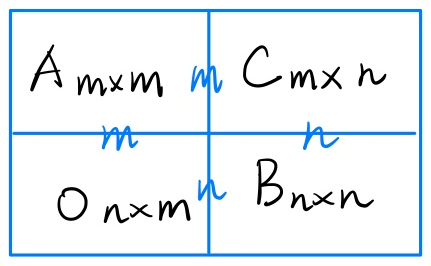
\includegraphics[width=0.2\textwidth]{img/0033.png}\\

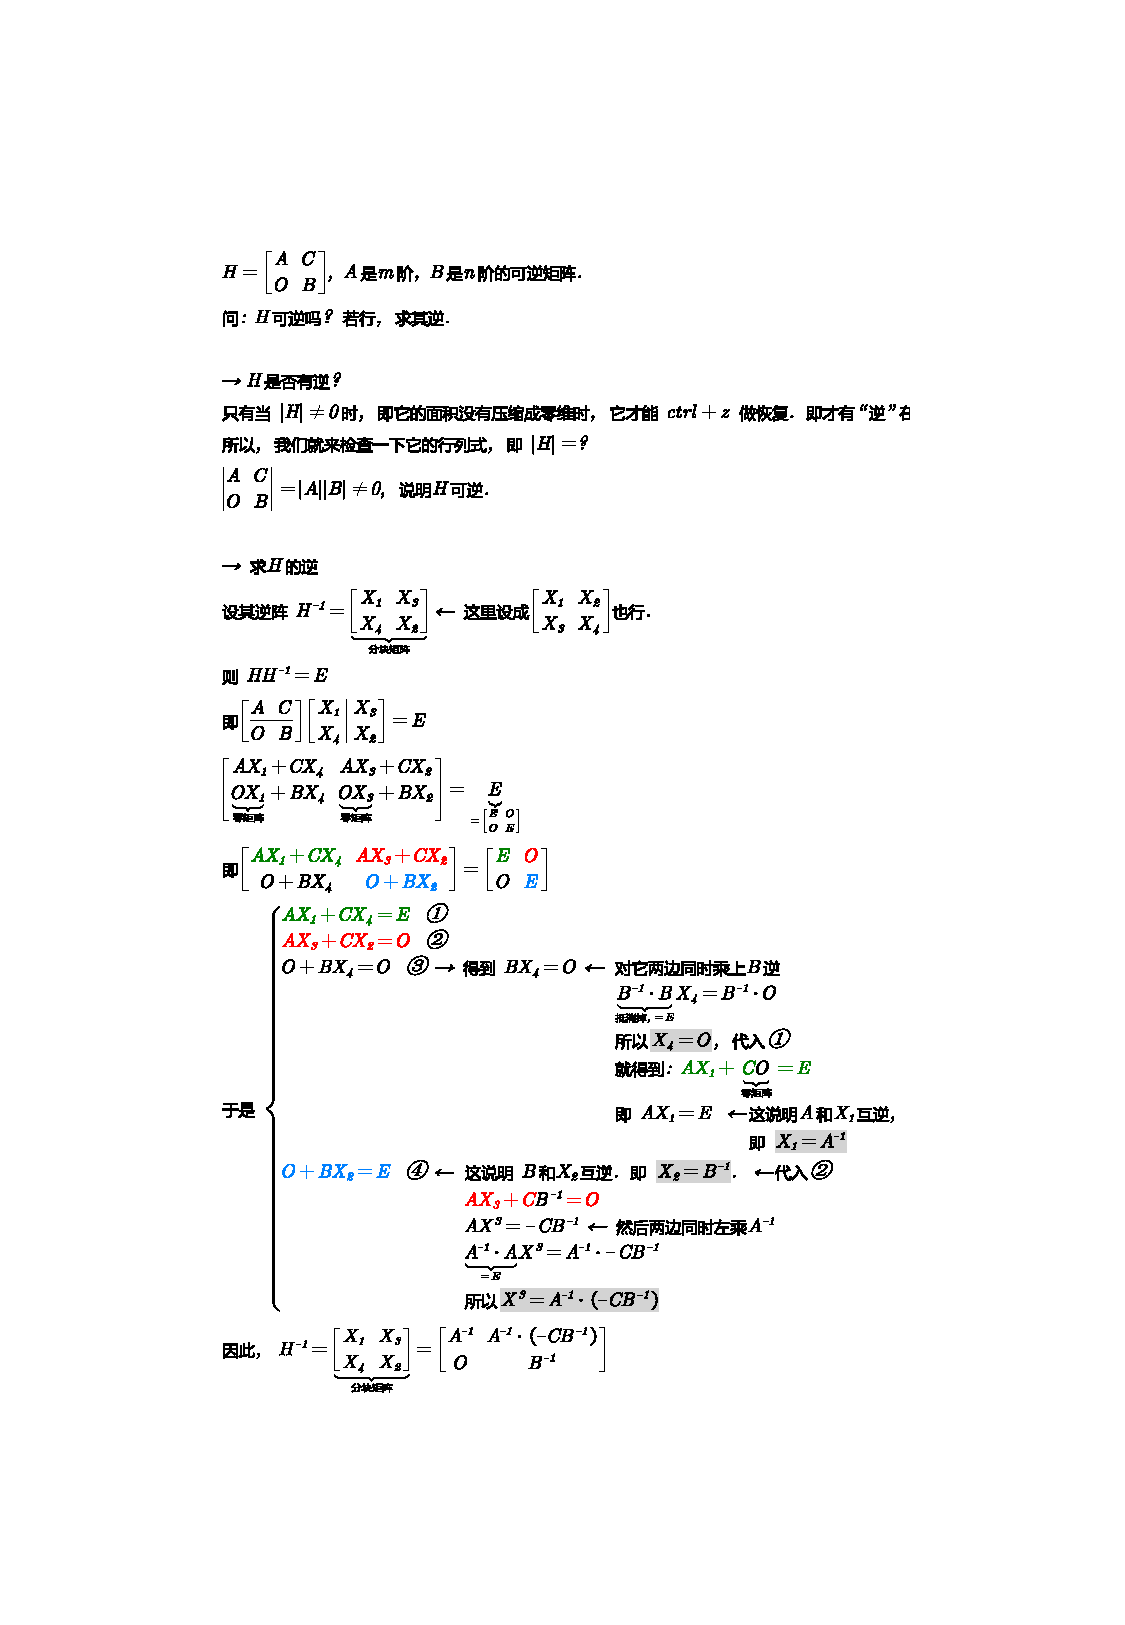
\includegraphics[width=1\textwidth]{img/0032.pdf}
\end{myEnvSample}


~\\
\hrule
~\\

\section{初等变换}

\subsection{初等变换, 有三种}

矩阵的初等变换 Elementary transformation, 有三种: \\

1.\textbf{交换两行.} \\
比如 $
\left[ \begin{matrix}
	1&		1&		1\\
	2&		2&		2\\
	4&		4&		4\\
\end{matrix} \right] \underrightarrow{\text{交换第1,2行}}\left[ \begin{matrix}
	2&		2&		2\\
	1&		1&		1\\
	4&		4&		4\\
\end{matrix} \right] 
$ \\
\vspace{1em} 

2.\textbf{用k($k \ne 0 $) 乘以某一行.} \\
$
\left[ \begin{matrix}
	1&		1&		1\\
	2&		2&		2\\
	4&		4&		4\\
\end{matrix} \right] \underrightarrow{line1 ×6}\left[ \begin{matrix}
	6&		6&		6\\
	2&		2&		2\\
	4&		4&		4\\
\end{matrix} \right] 
$ \\
\vspace{1em} 

3.\textbf{把某一行的k倍(k可为0), 加到另一行上去.} \\
$
\left[ \begin{matrix}
	1&		&		\\
	2&		\cdots&		\\
	4&		&		\\
\end{matrix} \right] \underrightarrow{newLine3=-4(line1)+(line3)}\left[ \begin{matrix}
	1&		&		\\
	2&		\cdots&		\\
	0&		&		\\
\end{matrix} \right] 
$\\
\vspace{1em} 

注意: 矩阵的``初等变换", 与行列式的初等变换, 没有任何关系. 虽然它们的三条变换规则相同.\\

任何矩阵, 都可以通过``初等变换", 变成``标准形" $
\left[ \begin{matrix}
	1&		&		&		&		&		\\
	&		\ddots&		&		&		&		\\
	&		&		1&		&		&		\\
	&		&		&		0&		&		\\
	&		&		&		&		\ddots&		\\
	&		&		&		&		&		0\\
\end{matrix} \right] 
$ 

\begin{myEnvSample}
	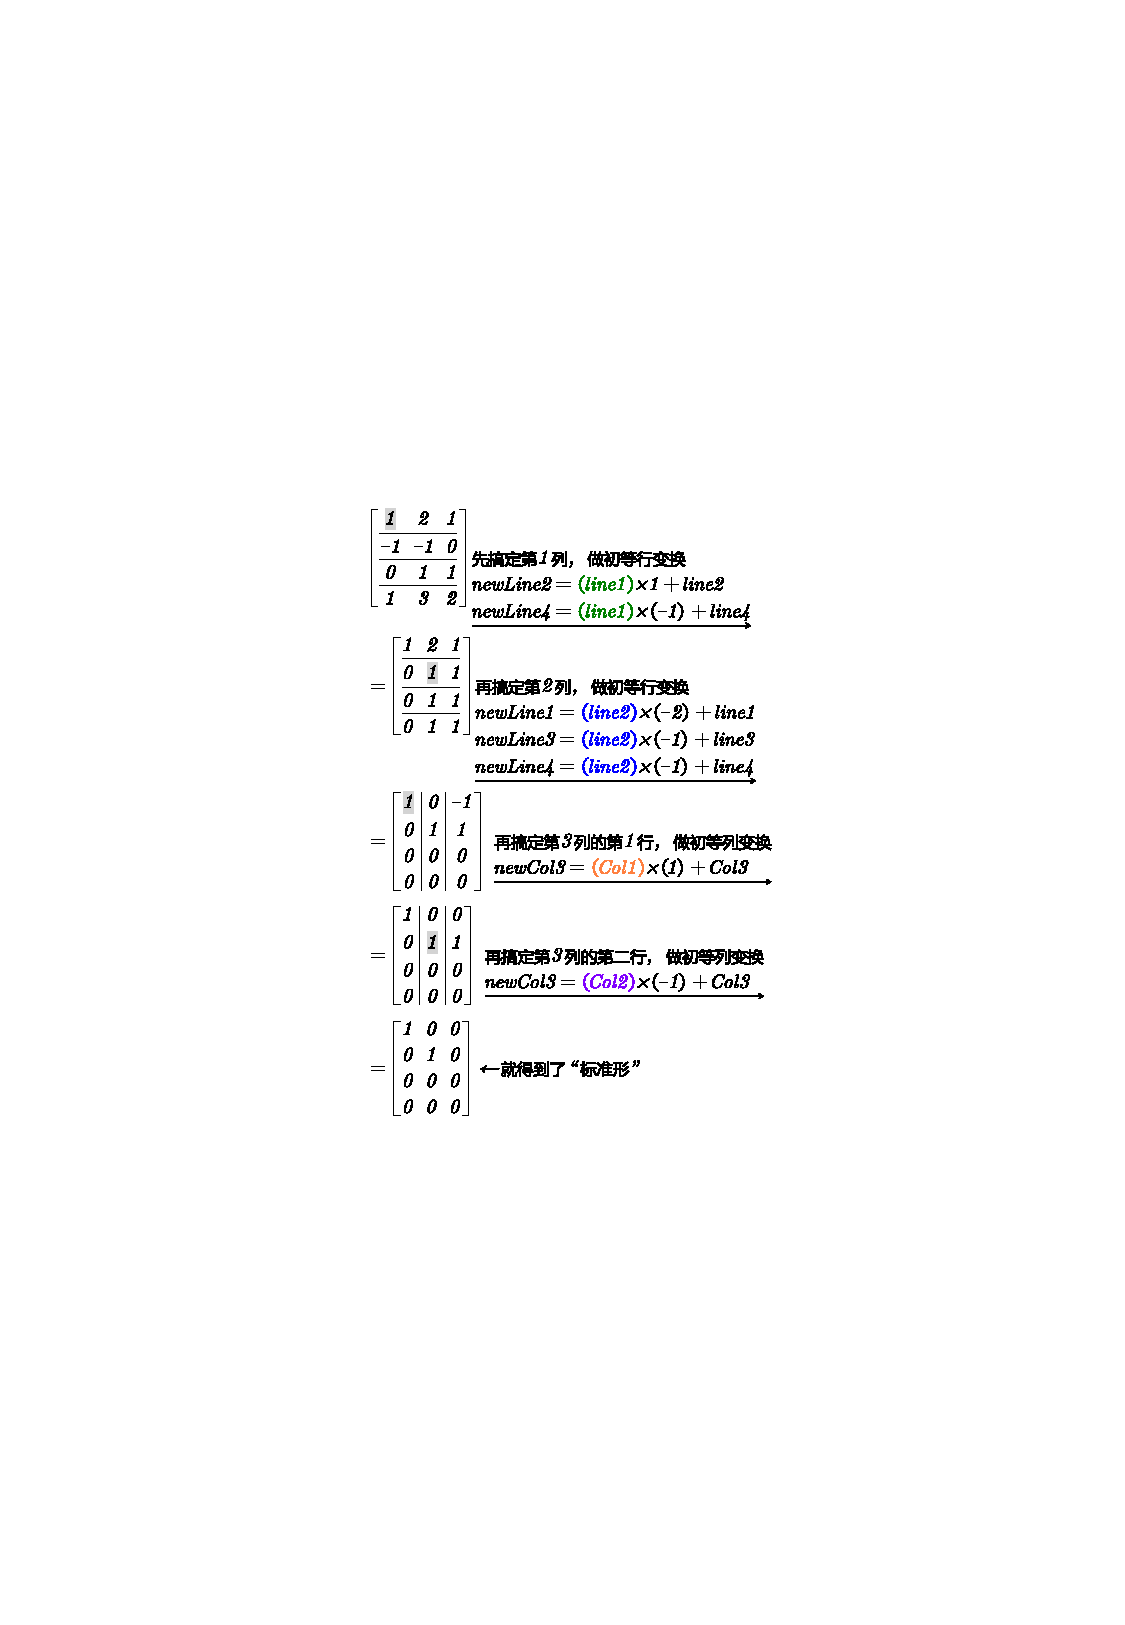
\includegraphics[width=0.6\textwidth]{img/0035.pdf}
\end{myEnvSample}

\hrule

\subsection{等价}

等价: A经过初等变换得到B, 则A与B等价. 记为 $A\cong B$.\\

等价的性质有: \\
1. 反身性: $A\cong A$  ← 自己等价于自己. \\
2. 对称性: $A\cong B$, 则 $B\cong A$. ← 重重就是说: A经过``初等变换"得到B, B也能再经过``初等变换"得回A. \\
3. 传递性: 若$A\cong B$, $B\cong C$, 则 $A\cong C$. ← 就相当于: A→C 的一步, 分成了两步来做. B只是中间状态而已. \\
4. 任意矩阵A $\cong $ 标准形 $\left[ \begin{matrix}
	1&		&		&		&		&		\\
	&		\ddots&		&		&		&		\\
	&		&		1&		&		&		\\
	&		&		&		0&		&		\\
	&		&		&		&		\ddots&		\\
	&		&		&		&		&		0\\
\end{matrix} \right] 
$ \\

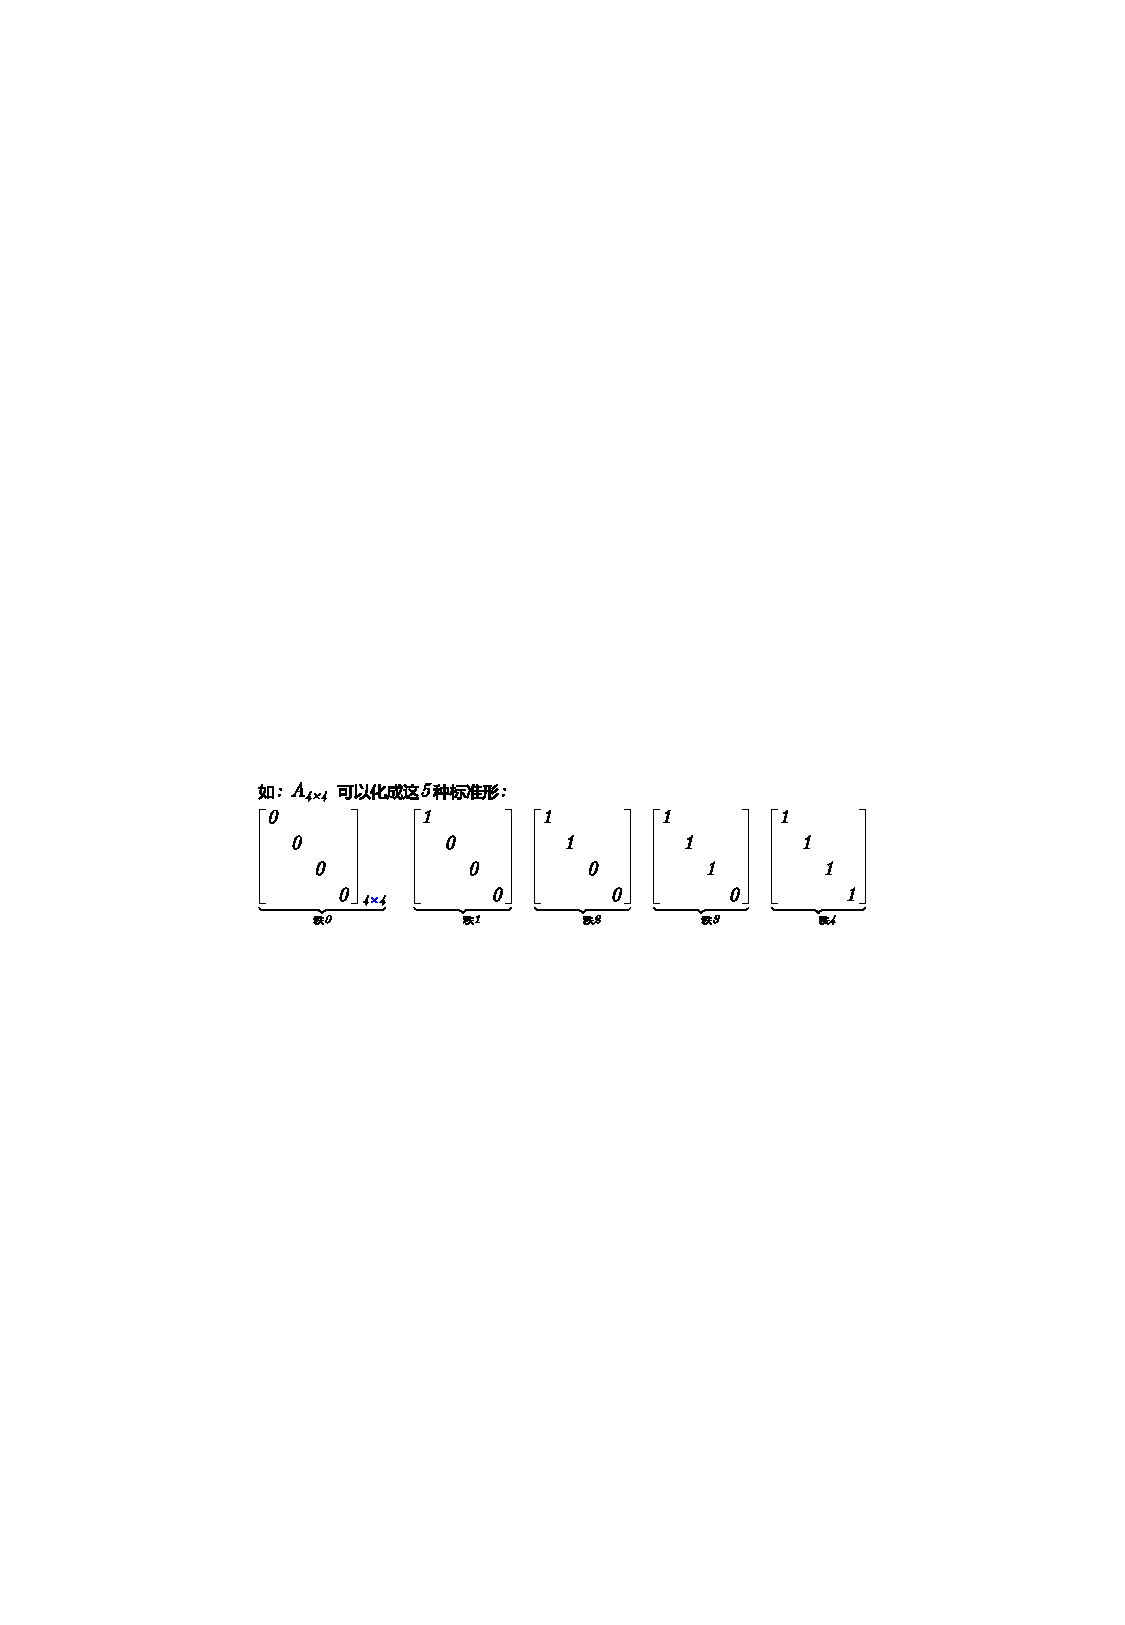
\includegraphics[width=0.8\textwidth]{img/0034.pdf}\\


\hrule

\subsection{初等方阵}

初等方阵 Elementary matrix: 对单位阵E 做一次``初等变换"得到的矩阵, 就是``初等方阵". \\

既然是做``初等变换", 就是3种了:

(1)\textbf{交换两行}:
\begin{align*}
	\left[ \begin{matrix}
		1&		&		&		\\
		\hline
		&		1&		&		\\
		&		&		1&		\\
		\hline
		&		&		&		1\\
	\end{matrix} \right] \overset{\text{交换1,3行}}{\rightarrow}\left[ \begin{matrix}
		&		&		1&		\\
		\hline
		&		1&		&		\\
		1&		&		&		\\
		\hline
		&		&		&		1\\
	\end{matrix} \right]
\end{align*}

记为: $ E(i,j)$ , 即交换``第i行"和``第j行"后, 所得到的矩阵.\\


(2)\textbf{用k 乘上某一行/列}
\begin{align*}
	\left[ \begin{matrix}
		1&		&		&		\\
		&		1&		&		\\
		&		&		1&		\\
		&		&		&		1\\
	\end{matrix} \right] \overset{newLine3\ =\ 5* line3}{\rightarrow}\left[ \begin{matrix}
		1&		&		&		\\
		&		1&		&		\\
		&		&		5&		\\
		&		&		&		1\\
	\end{matrix} \right]
\end{align*}


记为: $E(i(k))$ , 即把第i行, 变为k倍. $k \ne 0$.\\


(3)\textbf{某行的k倍, 加到另一行上去}
\begin{align*}
	\left[ \begin{matrix}
		1&		&		&		\\
		&		1&		&		\\
		&		&		1&		\\
		&		&		&		1\\
	\end{matrix} \right] \overset{newLine1\ =\ (5* line3)+line1}{\rightarrow}\left[ \begin{matrix}
		1&		&		5&		\\
		&		1&		&		\\
		&		&		1&		\\
		&		&		&		1\\
	\end{matrix} \right]
\end{align*}

记为:  $ E(i, j(k))$ , 即把 ``j行的k倍", 加到``第i行"上去.\\

\textbf{可以看出: 三种不同的变换方式, 所得到的``初等方阵", 其``行列式值", 是不同的.} \\

→ 第(1)种: 
$	\left[ \begin{matrix}
	&		&		1&		\\
	&		1&		&		\\
	1&		&		&		\\
	&		&		&		1\\
\end{matrix} \right] =-1$ ←即: $\boxed{|E(i,j)| = -1}$ \\
其逆阵是: $\boxed{E^{-1}(i,j) = E(i,j)}$\\
\vspace{1em} 

→ 第(2)种:
$\left[ \begin{matrix}
	1&		&		&		\\
	&		1&		&		\\
	&		&		5&		\\
	&		&		&		1\\
\end{matrix} \right] =5$  ← 即: $\boxed{ |E(i(k))| = k, (k \ne 0)}$\\
其逆阵是: $\boxed{E^{-1}(i(k)) = E(i(\frac{1}{k}))}$\\
\vspace{1em} 

→ 第(3)种:
$\left[ \begin{matrix}
	1&		&		5&		\\
	&		1&		&		\\
	&		&		1&		\\
	&		&		&		1\\
\end{matrix} \right] =1$ ← 即: $\boxed{|E(i, j(k))| = 1}$\\
其逆阵是: $\boxed{E^{-1}(i, j(k)) = E(i,j(-k))}$\\


上面三种初等变换得到的矩阵, 做出来的行列式值, 都不等于0. 说明: (1)它们(即初等方阵)都可逆. (2)它们的逆矩阵, 也是``初等方阵." (3)并且, 初等方阵的转置, 也是``初等方阵." \\



注意区别:\\
- 初等变换:  (v.) 是动词, 是对矩阵做``变换"的一种过程. \\
- 初等方阵: (n.) 是名词. 它就是一个方阵.\\



\begin{myEnvSample}
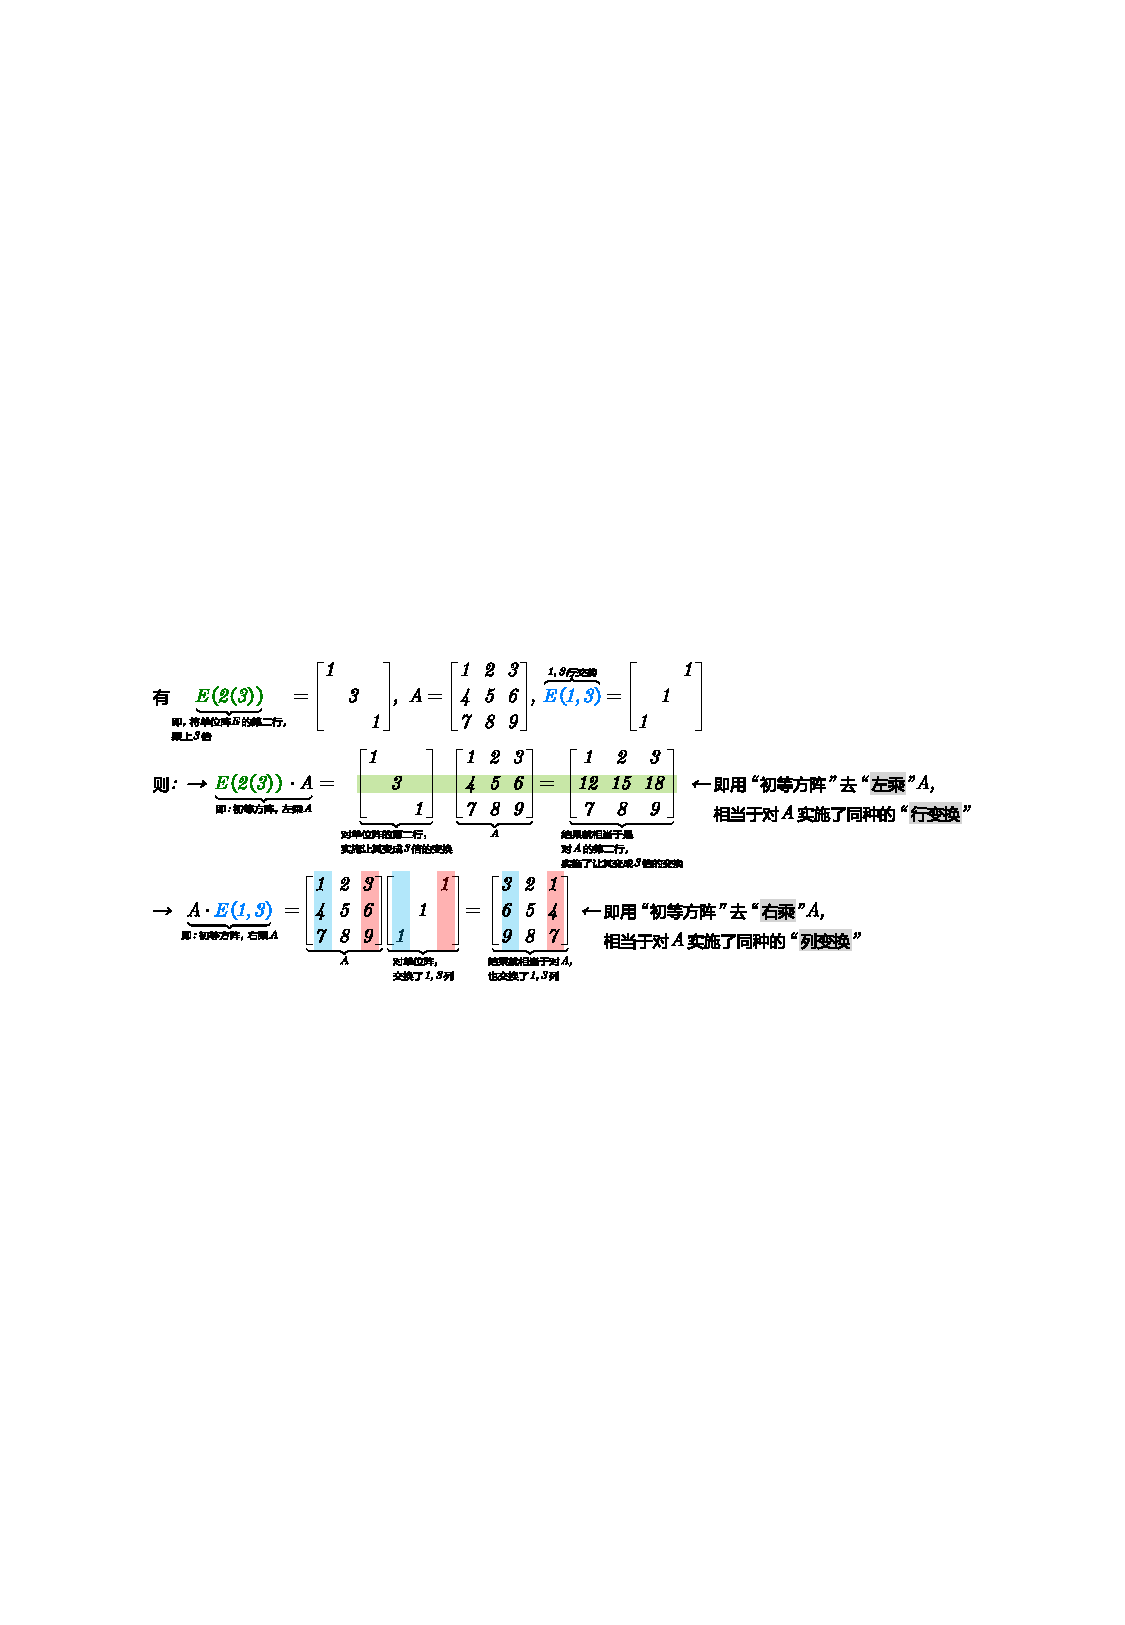
\includegraphics[width=1\textwidth]{img/0036.pdf}\\

这两个单位阵E, 做了一次``初等变换"后, 就已经是``初等方阵"了. 那么用``初等方阵"左乘``一个普通矩阵, 和``右乘"一个普通矩阵, 顺序不同, 运算规则也是不一样的:\\

(1)用初等方阵``左乘" A矩阵 (即初等方阵在A左边)\\
E在左边, 即: \textbf{用第i种初等方阵 ``左乘"A, 效果就相当于对 A 实施了同种的  (即也是第i种的)``初等行变换".} (左行,右列) \\
比如本例, 对E做了 ``对第2行, 乘上3倍" 的操作, 就相当于对A做了 ``对第2行, 乘上3倍" 的操作.\\

(2)用初等方阵``右乘" A矩阵 (即初等方阵在A右边)\\
E在右边, 即: \textbf{用第i种初等方阵 ``右乘"A, 效果就相当于对 A 实施了同种的 (即也是第i种的)``初等列变换".} (左行,右列)\\

\textbf{这就好像是古代的扎小人巫术, 对初等方阵E(人偶)做扎针, 就相当于对A(真人对象)做同等扎针.}
\end{myEnvSample}

数学研究中, 喜欢等号. 而初等方阵, 恰恰能提供等号.\\

~\\
\hrule
~\\

\subsection{定理: 对于任意一个矩阵A, 都存在``初等矩阵" $P_1, P_2, ..., P_s, Q_1, Q_2, ..., Q_t$, 能使得$	P_s\cdot ...\cdot P_1AQ_1\cdot ...Q_t	$ 为 ``标准形".}

因为任意矩阵A, 可以通过``初等变换"(行变换或列变换), 化为标准形. \\

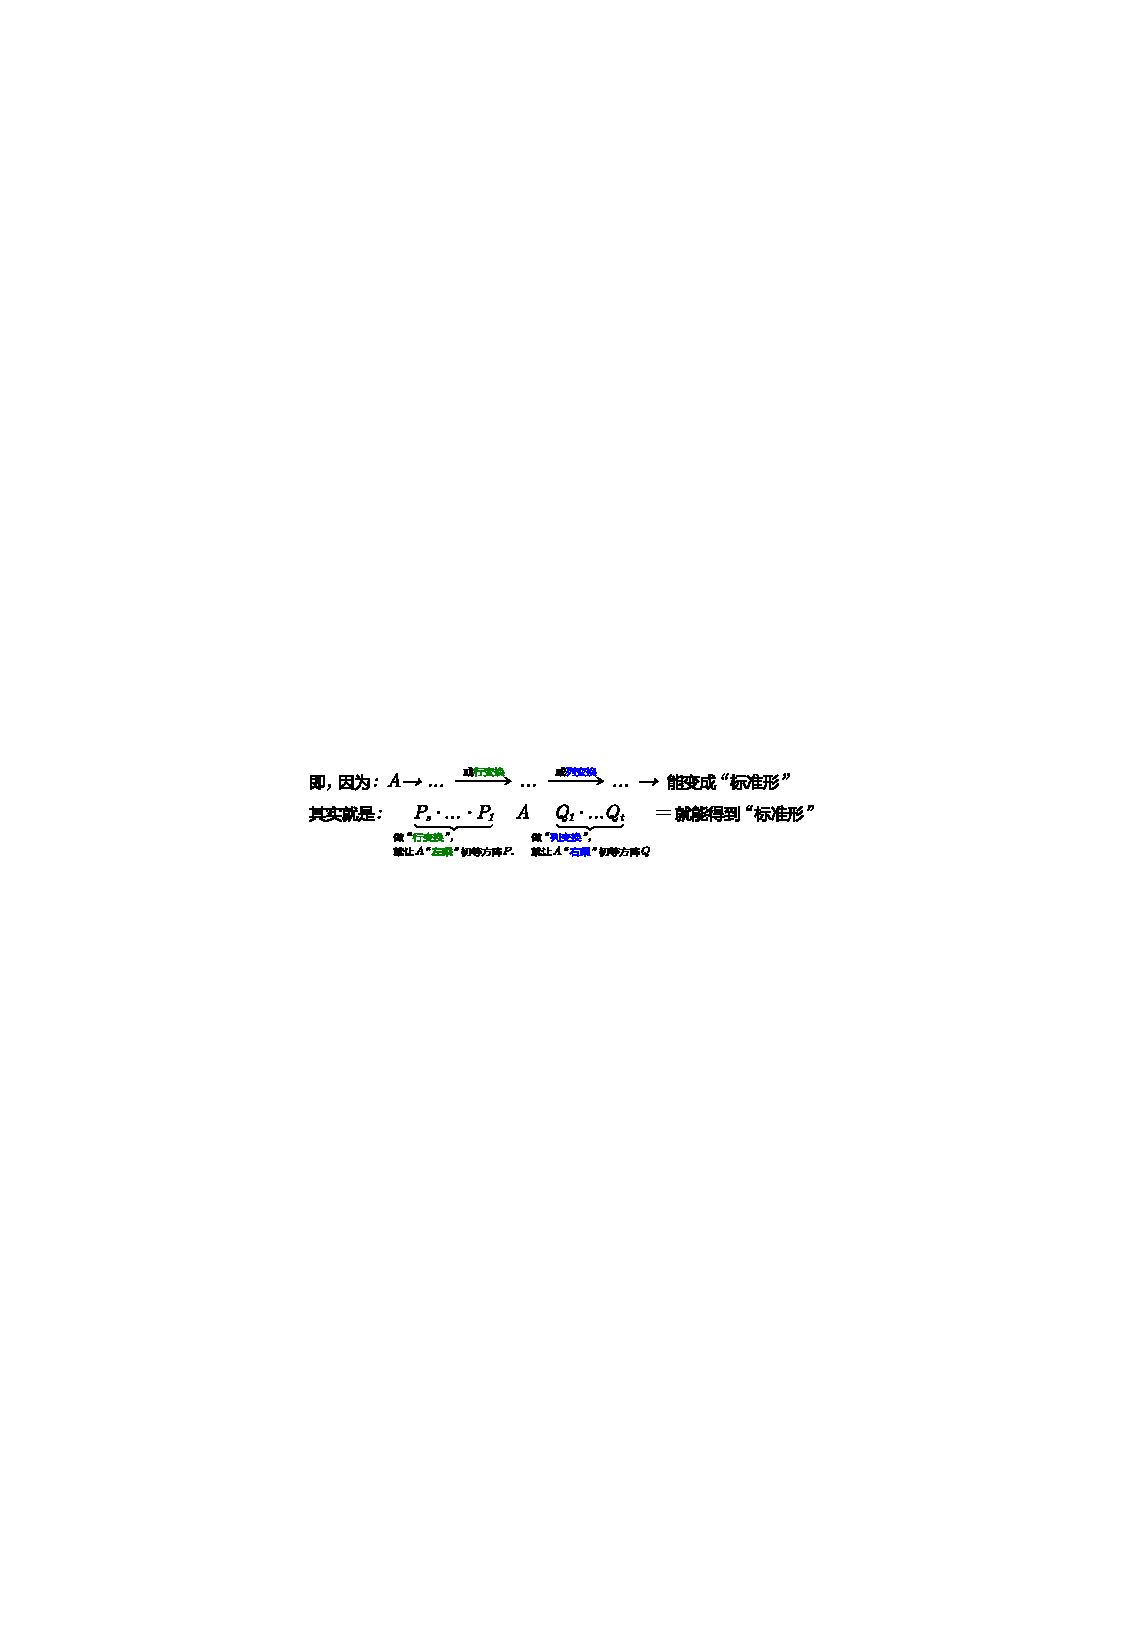
\includegraphics[width=0.75\textwidth]{img/0037.pdf}\\


\subsection{推论: 若A,B等价, 其充要条件是:  存在可逆矩阵P,Q, 使得 PAQ=B }

``A,B等价"的意思是: A通过``初等变换"(用初等行变换, 或初等列变换), 可以得到B. \\

所以, 在变换过程中, 如果用了``初等行变换", 就等价于是让A``左乘"初等方阵P(\textbf{初等方阵有这个性质: 初等方阵均可逆}). 如果用了``初等列变换", 就等价于让A``右乘"初等方阵Q. 即就有: $	P_s\cdot ...\cdot P_1AQ_1\cdot ...Q_t = B$\\



\subsection{定理: ``A可逆"的充分必要条件是: ``A的标准形"为单位阵E}

\begin{myEnvSample}
这个定理的证明过程如下: \\

若A可逆, 且标准形为D, 则存在初等方阵P,Q, 能使得: $	\underset{\text{初等方阵}}{\underbrace{P_s\cdot ...\cdot P_1}}A\underset{\text{初等方阵}}{\underbrace{Q_1\cdot ...Q_t}}=\underset{\text{标准形}}{\underbrace{D}}\\
$\\
我们对等号两边取行列式, 就有: $|P_s\cdot ...\cdot P_1AQ_1\cdot ...\cdot Q_t|=|D|$\\

等号左边, 因为根据性质: ``矩阵的乘积"的行列式, 等于``行列式的乘积", 即 : |AB|=|A||B|
 \\ 
所以就是:$ |P_s|\cdot ...\cdot |P_1|\cdot |A|\cdot |Q_1|\cdot ...\cdot |Q_t|=|D|$ \\


因为P,Q 是初等方阵, 初等方阵均``可逆", 而可逆的矩阵, 行列式值是不等于0的. 所以就有: $
\underset{\text{这里每一个矩阵都可逆,所以每一个行列式值都}\ne 0}{\underbrace{|P_s|\cdot ...\cdot |P_1|\cdot |A|\cdot |Q_1|\cdot ...\cdot |Q_t|}}=\underset{\text{所以它的行列式值,\ 也就}\ne 0\text{了}}{\underbrace{|D|}}
$ \\

而D是个标准形, 即: \\
$
\underset{\text{标准形}}{\underbrace{\left| \begin{matrix}
			1&		&		&		&		&		\\
			&		\ddots&		&		&		&		\\
			&		&		1&		&		&		\\
			&		&		&		0&		&		\\
			&		&		&		&		\ddots&		\\
			&		&		&		&		&		0\\
		\end{matrix} \right|}}
$ \\

上面这个标准形的行列式值要 $\ne 0$, 其对角线元素就不能存在0. 所以这个标准形, 就只能是形如下面的形式: \\
$
\underset{\text{标准形}}{\underbrace{\left| \begin{matrix}
			1&		&		&		&		&		\\
			&		\ddots&		&		&		&		\\
			&		&		1&		&		&		\\
			&		&		&		1&		&		\\
			&		&		&		&		\ddots&		\\
			&		&		&		&		&		1\\
		\end{matrix} \right|}}
$ ← 这个, 不就是单位阵E了么. 
\end{myEnvSample}



\subsection{定理: 若A可逆(即 $|A|\ne 0$), 则其充要条件是: A可以表示成``一些初等方阵的乘积". 即 $	A=P_1\cdot ...\cdot P_s	$}

~\\
\hrule
~\\


\section{矩阵的秩}

\subsection{rank 是什么? }

\subsubsection{秩 rank:是 ``行列式值是非零的"子式的最高阶数.}

rank 是: ``行列式值是非零的"子式的最高阶数.\\

\begin{myEnvSample}
比如: $A=\left[ \begin{matrix}
	1&		1&		1&		1\\
	2&		3&		4&		5\\
	2&		2&		2&		2\\
\end{matrix} \right]$\\

任取两行两列, 构成的子集, 就叫``2阶子式". 把每阶子式的``行列式值"算出来, 本例就有:\\
\begin{tabular}{|p{0.3\textwidth}|p{0.3\textwidth}|}
	\hline
	&  行列式值 \\
	\hline
所有的1阶子式	& 1,1,1,1 \\
	\hline
所有的2阶子式	& 假设为 -1,0,3... \\
\hline	
所有的3阶子式	& 假设为 0,0,0,0... \\
\hline		
\end{tabular}\\

本例中, 值为非零的子式的最高阶数, 只能取到2阶. 所有, 该矩阵的秩, 就是2.
\end{myEnvSample}

比如: \\
r(A)=r, 意思就是说: 它有一个r阶的子式不为0, 所有r+1阶的都为0, \\
r(A)=3, 意思就是说: 它有一个3阶的子式不为0, 所有4阶的都为0. \\




~\\
\hrule
~\\

\subsubsection{rank: 是已化为``阶梯形"的矩阵A中, 非零行的行数. = A的主元位置的个数 = A的主元列数}

r(A) = 阶梯形``非零行"的行数. \\
\textbf{把矩阵化为``简化阶梯行"后, 主元有几个, 该矩阵的rank 就是几.} 因为"初等行(或列)变换", 不会改变矩阵的 rank 数.

\begin{myEnvSample}
如: 
\begin{align*}
	A=\left[ \begin{matrix}
		1&		&		&		4\\
		&		1&		&		5\\
		&		&		1&		4\\
		&		&		&		\\
	\end{matrix} \right]
\end{align*}

该简化阶梯行, 有3个主元, r(A)=3.
\end{myEnvSample}


\textbf{其实, 也不需要化简到``简化阶梯形", 只要化到``阶梯形", 就能直接数一数非零行的行数, 就是该矩阵的``秩数"了.} \\


\begin{myEnvSample}
	求A的 rank数
	\begin{align*}
A=\left[ \begin{matrix}
	3&		3&		3\\
	2&		-1&		5\\
	-5&		3&		-13\\
	4&		-3&		11\\
\end{matrix} \right] \underset{\text{化为行阶梯形}}{\underbrace{\rightarrow }}\underset{\text{非零行有两行}}{\underbrace{\left[ \begin{matrix}
			1&		1&		1\\
			&		-3&		3\\
			&		&		\\
			&		&		\\
		\end{matrix} \right] }}
	\end{align*}
所以, rank(A)=2 = A的行秩 = A的列秩
\end{myEnvSample}


比如, A = O, 零矩阵, 其 rank(A) = 0
	
	
	
	
	~\\
	\hrule
	~\\
	
	
	\subsubsection{向量组的rank = ``极大线性无关组"中所含向量的个数}
	
	~\\
	\hrule
	~\\
	
	
	
\subsubsection{rank: 代表经过``线性变换"后, 新坐标系空间的维度. 即``新基坐标系"中的轴的数量}

对于 $ A\vec{x}=\vec{b}$, 当变换的结果, 将原坐标系压缩成一条直线时 (即``新基"中的轴, 共线了), 就称这个A(变换矩阵,新基矩阵) 的 rank = 1. \\

\includegraphics[width=0.6\textwidth]{img/0038.png}\\

如果变换后, 原向量都被落在一个二维平面上, 就称这个A(变换矩阵,新基矩阵) 的 rank = 2.  \\
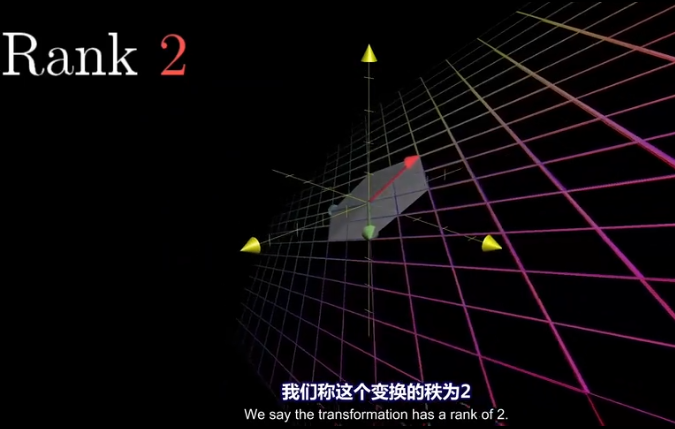
\includegraphics[width=0.6\textwidth]{img/0039.png}\\

对于3*3的矩阵, rank为2, 就意味着空间维度被压缩了.\\


\begin{myEnvSample}
$\left[ \begin{array}{c |c}
	3&		1\\
	4&		1\\
	5&		9\\
\end{array} \right]$ \\

该``新基矩阵", 它有两列, 说明是两个轴(有两个基向量)(比如 $\hat{i}, \hat{j}$). 但每个轴由三个数字表示, 即是处在三维空间的. 就说明它其实是把二维平面, 映射到了三维空间中.
\end{myEnvSample}



\begin{myEnvSample}
$\left[ \begin{array}{c|c|c}
	3&		1&		4\\
	1&		5&		9\\
\end{array} \right]$ \\

有3列, 表明``原始空间"中有3个基向量(即``原始空间"是三维的). 每个基向量, 由两个数字表示坐标, 表明这3个基向量, 在变换后, 都仅用两个坐标轴来表示. 所以原像一定落在二维平面中. 被降维了.\\

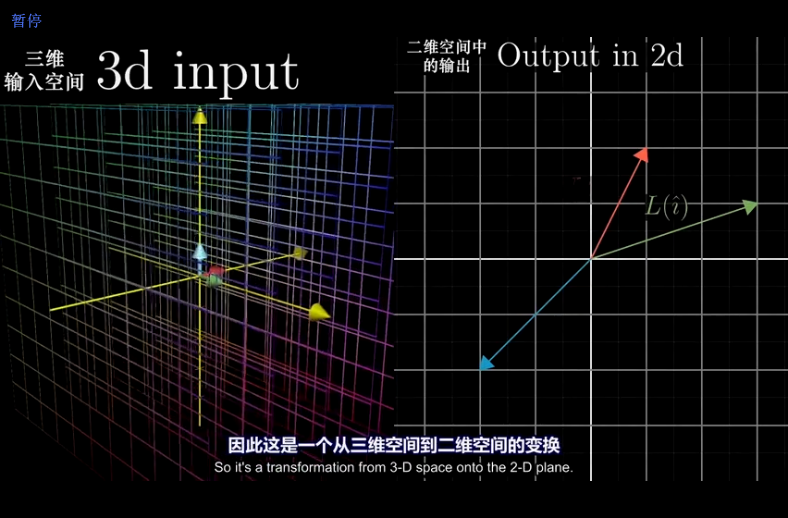
\includegraphics[width=0.6\textwidth]{img/0040.png}\\
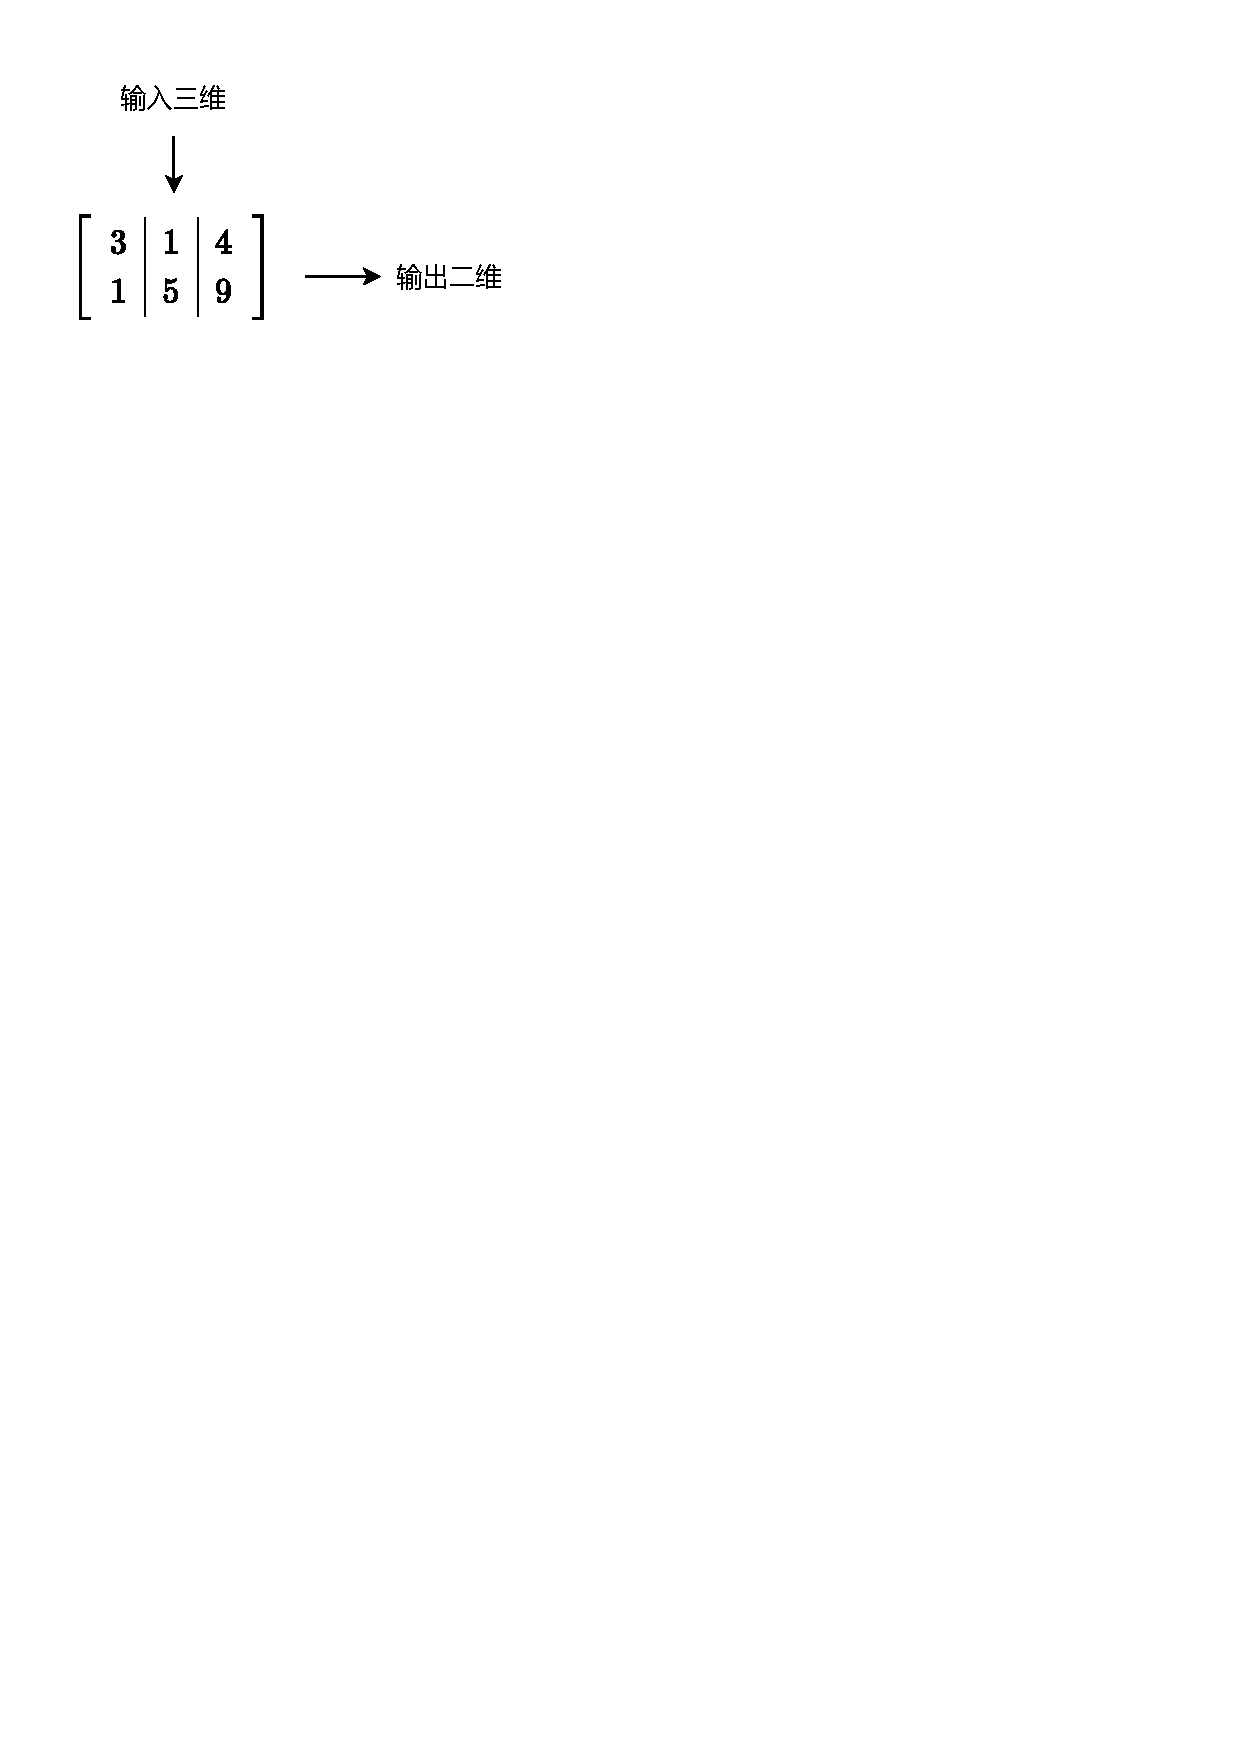
\includegraphics[width=0.35\textwidth]{img/0041.pdf}
\end{myEnvSample}



\begin{myEnvSample}
$\left[ \begin{array}{l}
	2\\
	7\\
\end{array} \right] \rightarrow L(\vec{v})\rightarrow \left[ \begin{matrix}
	1.8\\
\end{matrix} \right]$\\

输入二维, 输出一维\\
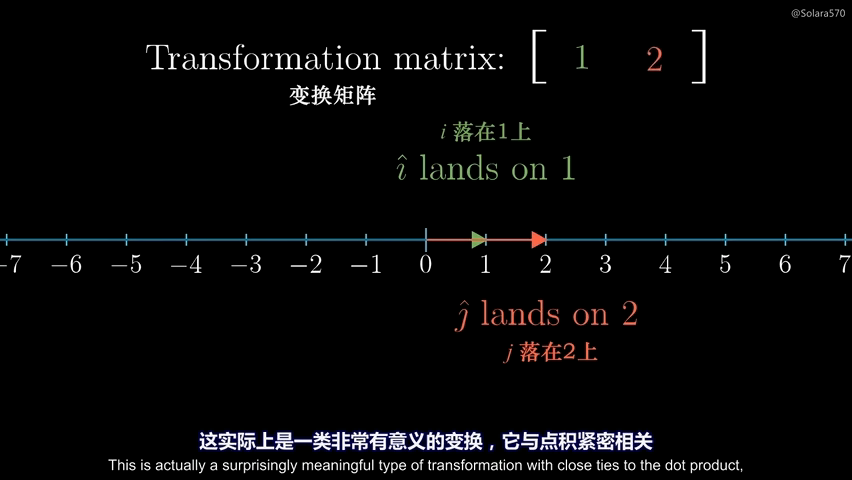
\includegraphics[width=0.6\textwidth]{img/0042.png}\\
\end{myEnvSample}


~\\
\hrule
~\\

\subsection{rank 有什么用? 它能告诉我们什么?}

\subsubsection{rank, 可以用来反映 matrix 结构的复杂性}

\begin{myEnvSample}
$A=\left[ \begin{matrix}
	1&		1&		1\\
	2&		2&		2\\
	3&		3&		3\\
\end{matrix} \right]$ \\

该矩阵, 实际上只用第一行就能完全表示其他两行了, 因为它们是成比例的关系. 所以, 这说明该矩阵有``冗余"信息, 其中的两行完全没有存在的必要. 核心信息行只有一行. 所以该矩阵的 rank 是1. \\
记为 r(A)=1. ← r() 就是一个函数, 它的功能是: 输入一个矩阵, 输出该矩阵的 rank数.
\end{myEnvSample}



\begin{myEnvSample}
$A=\left[ \begin{matrix}
	1&		1&		1&		1\\
	0&		2&		3&		4\\
	0&		0&		0&		9\\
\end{matrix} \right]$\\

该matrix, 三行缺一不可. 因为无法用其中一行来表示其他的行. 所以该矩阵的 rank=3.
\end{myEnvSample}


\begin{myEnvSample}
r(0矩阵) = 0
\end{myEnvSample}

一句话: 一个线性方程组, 去掉没用的冗余方程后, 最后剩下的方程个数, 就是秩.



\subsubsection{rank数, 能告诉我们, 方程组是否有解}

下面, 我们用$\overline{A} $来表示 矩阵A的``增广系数矩阵". n代表方程组中``未知元"的数量.\\

则有:\\
- 当 $ rank(A) = rank(\overline{A})$ 时, 方程组有解. \\
→ 若 $ rank(A) = rank(\overline{A}) = n$ 时, 有唯一解. \\
→ 若 $ rank(A) = rank(\overline{A}) < n$ 时, 有无穷多解. \\

- 当 $ rank(A) \ne rank(\overline{A})$ 时, 无解.\\


\begin{myEnvSample}
$\overline{A}=\left[ \begin{array}{cccc|c}
	1&		-1&		2&		-1&		3\\
	&		&		-5&		2&		-6\\
	&		&		&		&		4\\
\end{array} \right]$\\

竖线左边, 是矩阵A, 其秩, r(A) =2 \\
整体, 是增广系数矩阵, $rank(\overline{A}) = 3 $\\
$r(A) \ne  r(\overline{A}) $, 说明该方程组无解.
\end{myEnvSample}



\begin{myEnvSample}
$\overline{A}=\left[ \begin{array}{ccc|c}
	1&		3&		-7&		-8\\
	&		1&		-5&		-7\\
	&		&		1&		1\\
	&		&		&		0\\
\end{array} \right]$\\

竖线左边, 是矩阵A, 其秩, r(A) =3 \\
整体, 是增广系数矩阵, $ rank(\overline{A}) = 3$ \\
$ r(A) =  r(\overline{A}) = n =  3 $, 说明有解, 且唯一. \\
(n是未知元个数.)
\end{myEnvSample}


~\\
\hrule
~\\

\subsection{矩阵的 rank 数, 取值范围 :  $\boxed{
		0 \le r(A) \le min \{m,n\}}$}

有矩阵: $A_{m \times n}$,  则: $\boxed{
	0 \le r(A) \le min \{m,n\}}$ ← 即: \textbf{矩阵的秩数, 要比该矩阵的``行数或列数的最小者"要小.}\\

- 若$ r(A)=m$ : 说明其``非零(值)子式",能取到该 matrix 的所有的行. 一个不落. 即, 该矩阵是``行满秩"的. \\
\textbf{A是方阵, A``满秩"的充要条件是: A可逆, 即 $ |A| \ne 0 $.}\\

- 若 $ r(A)=n$ : 说明其``非零(值)子式",能取到该 matrix 的所有的列. 一个不落. 即, 该矩阵是``列满秩"的.\\

- 若$r(A) < min\{m,n\}$ : 说明就不是``满秩"的了, 而叫``降秩".







~\\
\hrule
~\\



\subsection{定理, 性质}


\subsubsection{矩阵A的行秩 = 列秩 = rank(A)}

把矩阵的每一行, 看做一个向量, 就是``行向量". 由这些``行向量"组成的向量组, 这个向量组的rank, 就是``行秩".\\
同理, 把矩阵的每一列, 看做一个向量, 就是``列向量". 由这些``列向量"组成的向量组, 这个向量组的rank, 就是``列秩".\\

可以证明: 一个矩阵的行秩 = 列秩 = 该矩阵的秩


~\\
\hrule
~\\



\subsubsection{$r(A) = r(A^T) $ ← 转置对秩数没有影响}


~\\
\hrule
~\\


\subsubsection{只要某一``子阶阶数"的行列式值, 已经为0了, 则所有比它``更高阶数的子阶"的行列式值, 一定都=0.}

\begin{myEnvSample}
如, 假设有一个3阶子式, 已经行列式值不为0了, 则所有3阶以上的子式, 不管是4阶, 5阶, ..., 它们的行列式值, 一定都=0.
\end{myEnvSample}


\begin{myEnvSample}
有 
$
	A=\left[ \begin{matrix}
		k&		1&		1&		1\\
		1&		k&		1&		1\\
		1&		1&		k&		1\\
		1&		1&		1&		k\\
	\end{matrix} \right]
$, 并且已知 r(A)=3, \\
那么显然, 该矩阵所有高于3阶的子式 的行列式值, 都=0. 因此, 该4阶矩阵的行列式值, 也就等于0了. 即:  |A| = 0.
\end{myEnvSample}


~\\
\hrule
~\\


\subsubsection{任意矩阵 × 可逆矩阵A  → 所得到的新矩阵的秩数, 和A的秩数相同}

即, 有 可逆矩阵 $ A_{m \times n}$, 还有 P 和 Q 这两个可逆的n阶方阵. 则有:\\
$r\left( A \right) =\underset{\text{p左乘于A}}{\underbrace{r\left( PA \right) }}=\underset{\text{Q右乘于A}}{\underbrace{r\left( AQ \right) }}=\underset{\text{P左乘, Q右乘于A}}{\underbrace{r\left( PAQ \right) }}$


~\\
\hrule
~\\


\subsubsection{r(AB) <= min{(r(A),r(B)}}

\textbf{两个矩阵相乘后的整体的rank数, 是小于等于``其中 rank数 最小的那个矩阵"的.} \\
同理, 推广到多个矩阵的情况,即: $ r(A_1 A_2 ... A_m) \leq min\{(r(A_1),r(A_2),...,r(A_m)\}$.


~\\
\hrule
~\\

\section{阶梯形矩阵}

阶梯形矩阵 Row-Echelon Matrix : 就是每行上, 左侧的0的个数, 必须要下行比上行0多!\\

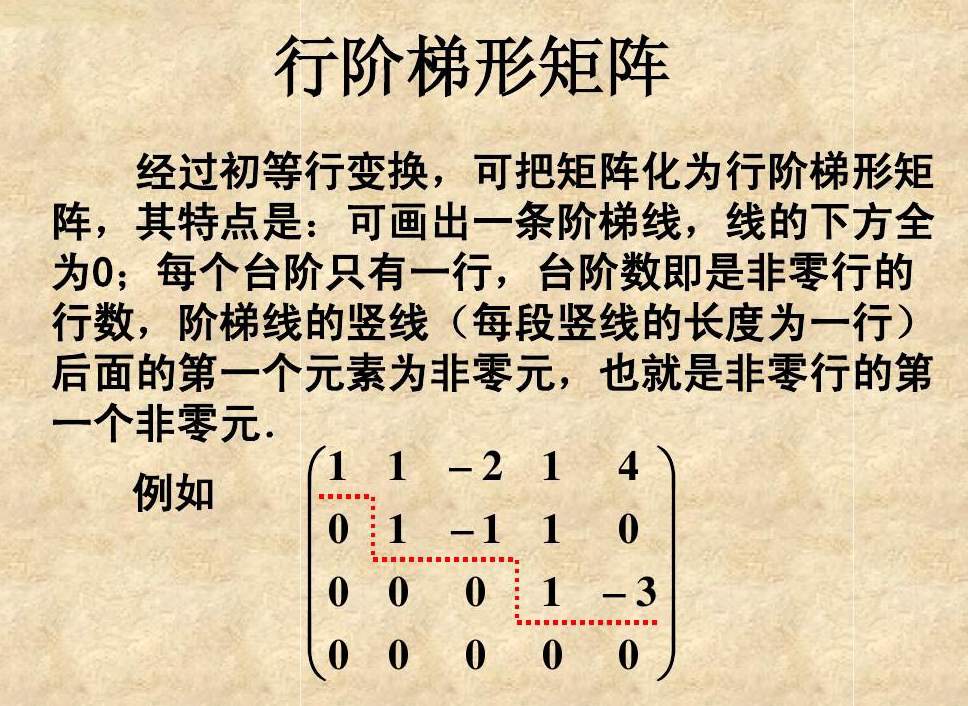
\includegraphics[width=0.5\textwidth]{img/0063.jpg}\\


比如, 下面这个矩阵就不满足``阶梯形矩阵"的要求:  \\
$A=\left[ \begin{matrix}\
	1&		&		&		&		\\
	&		1&		&		&		\\
	&		&		&		1&		\\
	&		&		&		3&		4\\
	&		&		&		&		\\
\end{matrix} \right]$\\

因为它的第3,4行, 左边的0一样多了. 而没满足``下行比上行的 0 严格增加"的要求.\\
即: 阶梯形矩阵, 水平\textbf{横线可跨多个数, 但竖线只能一步下一层台阶, 而不能一步下几层台阶.} \\


~\\
\hrule
~\\


\section{行简化阶梯形}

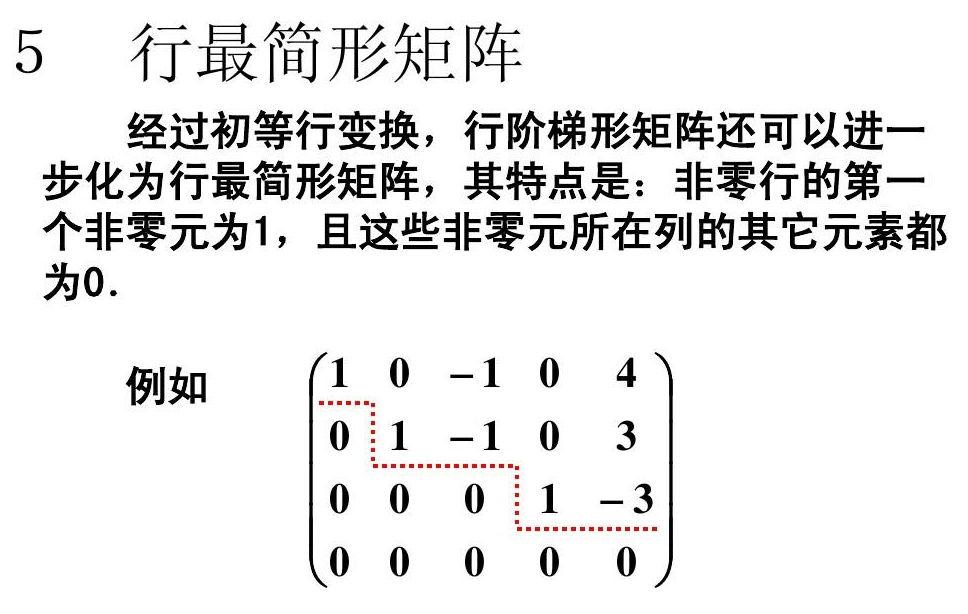
\includegraphics[width=0.5\textwidth]{img/0064.png}\\

有定理:\\
1.\textbf{矩阵的秩 r(A) = 非零行的行数.} 非零行有几行, 该矩阵的秩数就是几. \\
2.初等(行或列)变换, 不会改变矩阵的秩. 那么我们就可以不需要把矩阵一定化成``简化阶梯形"了, 只需化成"阶梯形", 数一数它的非零行有几行, 就是矩阵的秩数了. \\

\begin{myEnvSample}
	GeoGebra中, 可以用下面的命令, 来得到一个矩阵的简化阶梯形: \\
	简化阶梯形=ReducedRowEchelonForm(矩形)\\
	
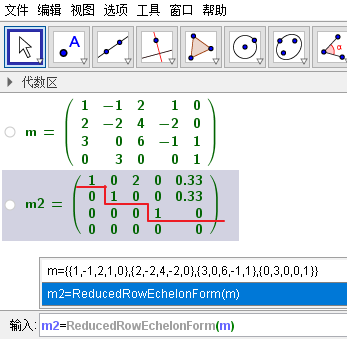
\includegraphics[width=0.4\textwidth]{img/0065.png} \\

所以该矩阵的秩 r(A)=3 ← 即非零行的行数.
\end{myEnvSample}

~\\
\hrule
~\\


\end{document}



